\documentclass[11pt,oneside,openany,a4paper,%..... Layout
               afrikaans, english%.............. Global language selection
               ]{memoir}

 \usepackage[PhD,%................................ PhD dissertation
             goldenblock,%........................ A5 type block (or a5block or wide)
            ]{usthesis}%.......................... US thesis style with memoir

\OnehalfSpacing

%
% PLEASE read the USthesis documentation for the class options
% and how to set line and paragraph spacing
%
%==== Language setup ================================================
 \usepackage[latin1]{inputenc}%................... Recognizes �, �, etc
 \usepackage{babel}%.............................. Language setup

%==== Math setup ====================================================
 \usepackage{amsmath}%............................ Advanced math (before fonts)
 \usepackage{amssymb}%............................ AMS Symbol fonts

%==== Font setup (default is Computer Modern) =======================
 \usepackage[T1]{fontenc}%........................ Type 1 fonts
 \usepackage{textcomp}%........................... Additional text character
 \usepackage{bm}%................................. Bold math symbols (after fonts)

%==== Ref's, Bib's and Nomencl ======================================
 \usepackage{usnomencl}%.......................... List of symbols (in usthesis pack)
 \usepackage{cite}

%==== Graphics and Color ============================================
  \usepackage[pdftex]{graphicx}
  \graphicspath{{../Figures/}}
%  \DeclareGraphicsExtensions{.pdf,.png}
  \usepackage{color}
  
\usepackage{color}%.............................. Color setup
\usepackage{eso-pic}%............................ Shipout commands for watermark
    \newcommand*{\WaterMark}[2][0.2\paperwidth]{%
        \AddToShipoutPicture*{\AtTextCenter{%
                \parbox[c]{0pt}{\makebox[0pt][c]{%
                    \includegraphics[width=#1]{#2}}}}}}

%==== Local Defs ====================================================
\makeatletter

%
% Please insert user defined commands here
% and NOT in the document itself!
%
\usepackage[caption=false]{subfig}

\renewcommand{\UScaptionsafrikaans}{%
    \def\DeclarationName{Verklaring}%
    \def\AbstractName   {Samevatting}%
}

%Add elegant support for Big-O notation
\providecommand{\OO}[1]{\operatorname{O}\left(#1\right)}

%\usepackage{listings}

% generate nice bookmarks and hyperrefs when exporting to pdf and dvi (screen version):
\usepackage[a4paper,plainpages=false,colorlinks,linktocpage,bookmarks=true,bookmarksopen=false]{hyperref}
% use this for printing only (no color, print version):
%\usepackage[a4paper,plainpages=false,colorlinks=false,linktocpage,bookmarks=true,bookmarksopen=false]{hyperref}

%\renewcommand{\lstlistlistingname}{List of Listings}

\hyphenation{MATLAB}

\makeatother

%==== TITLE PAGE ====================================================
\title{\AorE{%-- Afrikaans ------------------------------------------
             'n Toestandsbestuur en Stoor Argitektuur vir Eweknie Grootskaalse Multigebruiker Virtuele Omgewings \\[1ex]
             \normalfont\small\itshape
             (``A State Management and Persistency Architecture for Peer-to-Peer Massively Multiuser Virtual Environments'')
            }{%-- English -------------------------------------------
             A State Management and Persistency Architecture for Peer-to-Peer Massively Multiuser Virtual Environments
            }}

\author{J.S.\ Gilmore}{John Sebastian Gilmore}

\ThesisDescript{Dissertation presented for the degree of Doctor of Philosophy in the Faculty of Engineering at Stellenbosch University}

\degree{\AorE{PhD}{PhD}}
       {\AorE{\\Doktor van Filosofie}
             {\\Doctor of Philosophy}}

%\address{\AorE{%-- Afrikaans ----------------------------------------
%        Departement Elektries en Elektroniese Ingenieurswese,\\
%        Universiteit van Stellenbosch,\\
%        Privaatsak X1, 7602 Matieland, Suid Afrika.
%              }{%-- English ------------------------------------------
%         Department of Electrical and Electronic Engineering,\\
%         University of Stellenbosch,\\
%         Private Bag X1, 7602 Matieland, South Africa.
%              }}

\supervisor{Dr.\  Herman\ A. Engelbrecht}
\setdate{12}{2012}

%====================================================================
%     MAIN DOCUMENT
%====================================================================
\maxsecnumdepth{subsubsection}
\maxtocdepth{subsubsection}

\begin{document}

%==== Front matter ==================================================
 \frontmatter
 \WaterMark{UScrest-WM}
 \begin{SingleSpace}
    \TitlePage
 \end{SingleSpace}

\DeclarationPage[By submitting this dissertation electronically, I declare that the entirety of the work contained therein is my own, original work,
that I am the sole author thereof (save to the extent explicitly otherwise stated), that reproduction and publication thereof by Stellenbosch
University will not infringe any third party rights and that I have not previously in its entirety of in part submitted it for obtaining any
qualifications.]

 
\chapter*{Abstract}
Stellenbosch University and the Katholieke Universiteit Leuven has a joint undertaking to develop
a satellite communications payload. The goals of the project are: to undertake research
and expand knowledge in the area of dynamically configurable antenna beam forming, to prove
the viability of this research for space purposes and to demonstrate the feasibility of the
development in a practical application.

The practical application is low Earth orbit satellite communication system for applications in remote monitoring.
Sensor data will be uploaded to the satellite, stored and forwarded to a central processing
ground station as the satellite passes over these ground stations. The system will utilise many
low-cost ground sensor stations to collect data and distribute it to high-end ground stations
for processing.

Applications of remote monitoring systems are maritime- and climate change monitoring-
and tracking. Climate change monitoring allows inter alia, for the monitoring of the effects and causes
of global warming.

The Katholieke Universiteit Leuven is developing a steerable antenna to be mounted on the
satellite. Stellenbosch University is developing the communications payload to steer and use
the antenna. The development of the communications protocol stack is part of the project.
The focus of this work is to implement the application layer protocol, which handles all file level
communications and also implements the communications strategy.

The application layer protocol is called the \emph{Satellite Communications Software System}
(SCSS). It handles all high level requests from ground stations, including requests to store
data, download data, download log files and upload configuration information. The design
is based on a client-server model, with a \emph{Station Server} and \emph{Station Handler}.
The Station Server schedules ground stations for communication and creates a Station Handler
for each ground station to handle all ground station requests. During the design, all file
formats were defined for efficient ground station-satellite communications and system administration.
All valid ground station requests and handler responses were also defined.

It was also found that the system may be made more efficient by scheduling ground stations
for communications, rather than polling each ground station until one responds. To be able
to schedule ground station communications, the times when ground stations will come into
view of the satellite have to be predicted. This is done by calculating the positions of the
Satellite and ground stations as functions of time. A simple orbit propagator was developed to
predict the satellite distance and to ease testing and integration with the communications system.
The times when a ground station will be within range of the satellite were then predicted and
a scheduling algorithm developed to minimise the number of ground stations not
able to communicate.

All systems were implemented and tested. The SCSS executing on the Satellite was
developed and tested on the satellite on-board computer. Embedded implementations possess
strict resource limitations, which were taken into account during the development process.
The SCSS is a multi-threaded system that makes use of thread cancellation to improve
responsiveness.


\chapter*{Samevatting}
\hyphenation{grond-sta-sies}

Die Universiteit van Stellenbosch ontwerp tans 'n satelliet kommunikasieloonvrag in
samewerking met die Katolieke Universiteit van Leuven. Die doel van die projek is om
navorsing te doen oor die lewensvatbaarheid van dinamies verstelbare antenna bundelvorming
vir ruimte toepassings, asook om die haalbaarheid van hierdie navorsing in die praktyk
te demonstreer.

Die praktiese toepassing is 'n satellietkommunikasiestelsel vir afstandsmonitering,
wat in 'n Lae-Aarde wentelbaan verkeer. Soos die satelliet in sy wentelbaan beweeg,
sal sensor data na die satelliet toe gestuur, gestoor en weer aangestuur word. Die
stelsel gebruik goedkoop sensorgrondstasies om data te versamel en aan te stuur na
kragtiger grondstasies vir verwerking.

Afstandsmoniteringstelsels kan gebruik word om klimaatsverandering, sowel as die
posisie van skepe en voertuie, te monitor. Deur oa. klimaatsveranderinge te dokumenteer,
kan gevolge en oorsake van globale verhitting gemonitor word.

Die Katholieke Universiteit van Leuven is verantwoordelik vir die
ontwerp en vervaardiging van die satelliet antenna, terwyl die Universiteit van
Stellenbosch verantwoordelik is vir die ontwerp en bou van die
kommunikasie loonvrag. 'n Gedeelte van hierdie ontwikkeling sluit die
ontwerp en implementasie van al die protokolle van die
kommunikasieprotokolstapel in. Dit fokus op die toepassingsvlak
protokol van die protokolstapel, wat alle le\^{e}rvlak kommunikasie
hanteer en die kommunikasiestrategie implementeer.

Die toepassingsvlaksagteware word die Satellietkommunikasie sagtewarestelsel
(SKSS) genoem. Die SKSS is daarvoor verantwoordelik om alle navrae
vanaf grondstasies te hanteer. Hierdie navrae sluit die
oplaai en stoor van data, die aflaai van data, die aflaai van logs en
die oplaai van konfigurasie inligting in. Die ontwerp is op die standaard
kli\"{e}nt-bediener model gebasseer, met 'n \emph{stasiebediener} en 'n
\emph{stasiehanteerder}. Die stasiebediener skeduleer die tye wanneer
grondstasies toegelaat sal word om te kommunikeer en skep stasiehanteerders om alle
navrae vanaf die stasies te hanteer. Gedurende die ontwerp is alle
le\^{e}rformate gedefinieer om doeltreffende adminstrasie van die
stelsel, asook kommunikasie tussen grondstasies en die satelliet te
ondersteun. Alle geldige boodskappe tussen die satelliet en grondstasies
is ook gedefnieer.

Daar is gevind dat die doeltreffendheid van die stelsel verhoog kan word deur die
grondstasies wat wil kommunikeer te skeduleer, eerder as om alle stasies
te pols totdat een reageer. Om so 'n skedule op te stel, moet die tye
wanneer grondstasies binne bereik van die satelliet gaan wees voorspel
word. Hierdie voorspelling is gedoen deur die posisies van die
satelliet en die grondstasies as funksies van tyd te voorspel. 'n
Eenvoudige satelliet posisievoorspeller is ontwikkel om toetsing en
integrasie met die SKSS te vergemaklik. 'n Skeduleringsalgoritme is toe
ontwikkel om die hoeveelheid grondstasies wat nie toegelaat word om te
kommunikeer nie, te minimeer.

Alle stelsels is geimplementeer en getoets. Die SKSS, wat op die
satelliet loop, is ontwikkel en getoets op die satelliet se aanboord
rekenaar. Die feit dat ingebedde stelsels oor baie min hulpbronne beskik,
is in aanmerking geneem gedurende die ontwikkeling en implementasie van die SKSS.
Angesien die SKSS 'n multidraadverwerkingsstelsel is, word daar van
draadkansellasie gebruik gemaak om die stelsel se reaksietyd te verbeter.


\chapter{Acknowledgements}%==================================================

I would like to express my sincere gratitude to the following people and organisations:
\begin{itemize}
  \item the Holy Father, for keeping me and blessing me with so much;
  \item my study leader, Dr Riaan Wolhuter, for his continued guidance and support;
  \item my fianc\'{e}e, Jacki van der Merwe, for her lasting love, support and understanding;
  \item Francois Olivier and Shaun Lodder, for their valuable input during the late nights in the lab;
  \item Dr Gert-Jan van Rooyen for his valuable feedback on the SCSS design;
  \item Ewald van der Westhuizen for managing the Leuven project and for providing technical assistance;
  \item Kobus Botha for always being ready to assist with technical issues;
  \item Japie Engelbrecht, for helping me better understand satellite communication systems;
  \item the Telkom Centre of Excellence and Stellenbosch University, for their financial aid;
  \item my parents, John and Coreen Gilmore, for making me the man I am today and making
  my studies possible;
  \item the QNX support team, for their prompt and knowledgeable assistance with QNX related implementation issues;
  \item James Clark, for writing the Expat XML parser library;
  \item Jean-Loup Gailly and Mark Adler, for writing the zlib compression library.
\end{itemize}


\chapter{Dedications}%=======================================================
 \vfill
 \begin{center}\itshape
    In memory of my mother, Anita Gilmore, and my grandparents: Herman Kotze, Kotie Kotze and Hettie Gilmore.
	I hope I've made you proud.
 \end{center}
 \vfill
 \clearpage

%============================================================================
\endinput


 \tableofcontents
 \clearpage

 \setcounter{lofdepth}{2}
 \listoffigures
  \clearpage

  \listoftables
\clearpage

\chapter{Nomenclature}

\newlength{\gnat}
\settowidth{\gnat}{$GS_\textrm{dropped}$}

\begin{Nomencl}[\gnat]

\NomGroup{Some symbols}
		\item[$\phi$]		The greek letter phi
		
\NomGroup{Abbreviations}
		\item[TLA]			Three Letter Acronymn
\end{Nomencl}
\endinput


%==== Main document =================================================
\mainmatter
   \setsecnumdepth{subsubsection}
   \numberwithin{equation}{section}
   \numberwithin{figure}{chapter}
   \numberwithin{table}{chapter}

\chapter{Introduction}
\label{chp:INTRO}

\section{Massively Multi-user Virtual Environments}

Massively multi-user virtual environments (MMVEs) are characterised by thousands of users interacting in the same virtual environment or game world; socially, cooperatively or competitively. MMVEs can be serious, such as air traffic control simulations and military war games or casual, such as computer games. MMVEs as computer games are referred to as massively multiplayer online games (MMOGs) and can themselves be hardcore, where significant investments of time and money are required, or casual, where little time and money are required.

With the advent of broadband Internet, MMOGs have seen tremendous growth over the past decade, growing from less than 500,000 active subscribers in 1999 to over 21 million in 2011 \cite{mmo_growth_chart}. In 2011, the MMOG market was a \$2,6 billion industry in the United States alone \cite{newzoo_mmo_report}. MMOGs are characterised by expansive worlds, where a large number of players interact online with each other and the virtual environment to achieve certain goals through collaboration and teamwork.

From an academic perspective, MMOGs also hold great value. An MMOG is a complex networked application, with clients requiring reliable real-time feedback on actions taken. The design of an MMOG requires in-depth knowledge of server architectures and network design. The design of a server architecture determines how many players the game will support and what the user experience will be in terms of quality of service.

\subsection{Modern MMOG implementations}
\label{modern_mmogs}

\subsubsection{World of Warcraft (Fantasy MMORPG)}

Throughout the development of MMOGs, role play has been tightly coupled to this type of game. This is perhaps due to the exploration and player interaction aspects. Role play allows players to fully immerse themselves in the game world and might, therefore, provide for a more compelling experience. Because of this tight coupling, the terms massively multiplayer online role-playing game (MMORPG) and MMOG have almost become synonymous. Throughout this work, a distinction will, however, be made between the two, where MMORPG refers to the specific genre and MMOG refers to the ``massive'' and ``online'' characteristics of the game.

An MMORPG that has been very lucrative and has become well known in Western culture is Blizzard's World of Warcraft (WoW). In WoW, players are represented by avatars that inhabit a virtual fantasy world. An avatar has a race, a class, attributes, skills and professions. In the virtual world there are quests that a player may undertake to gain experience in classic RPG style. Gaining experience allows a player to gain levels, which improves its skills and attributes, making the player more powerful.

There are different reasons why players play the game. Some players play the game socially, to meet new people and make friends, other players play the game to become sufficiently powerful to play the end-game content. End-game content requires large groups of players to work together in a highly coordinated way to achieve some set of objectives, usually culminating in destroying a ``boss''. This activity is called ``raiding'', which is usually done by groups of players that have decided to play together and form a ``guild''. Guilds have complex social structures, which allows for various social interactions. Usually it is this high degree of social interaction that attracts players to MMOGs. Players are no longer playing by themselves in a lonely world, but rather playing with other players in a large open virtual space, waiting to be explored.

When a character is created in WoW, the creator must first choose a server on which the character will be stored. Characters on different servers cannot interact in the virtual world and cannot easily move between virtual worlds. Every server, which itself is a server cluster, hosts a complete copy of the virtual world. From a character perspective, the fact that there exists multiple copies of the game world is not know. This is termed sharding and will be discussed in detail in Section \ref{sharding}.

After eight years of operation, WoW still has 10,2 million subscribers, each paying \$15 per month subscription \cite{wow_firstq_fin_results_2012}.

\subsubsection{Eve online (Space MMORPG)}

Eve Online, developed by CCP Games, brought many new innovations to the MMORPG. It was the first successful MMORPG to feature a science fiction theme. It was the first MMOG to have a single distributed server architecture. In 2006, CCP Games launched the largest supercomputer in the gaming industry to upgrade their existing infrastructure and enable Eve to support more than 50,000 concurrent users \cite{eve_launces_supcom}. This number was surpassed in 2010 with 60,453 concurrent users in-game \cite{eve_pcu}.

Another innovation of Eve was the in-game economy. CCP games appointed Dr. Eyj\'{o}lfur Gu\~{o}mundsson as chief economist of Eve online in 2006 \cite{eve_economist}. His duties were to monitor and predict market trends in the game world and produce detailed quarterly economic reports \cite{eve_econ_rep}.  The economy is based on an open market system, ruled by supply and demand. No other game has implemented an in-game economy in such a rigourous fashion.

\subsubsection{Second life (MMOSG)}

Second life is classified as a massively multiplayer online social game (MMOSG). It focusses more on social interaction and creatively, as opposed to the usual conflict-based MMORPGs, such as WoW or Eve online. Players in Second Life can create virtual items, such as clothing, furniture and architecture, and sell them them for real money. Players can buy property and build on the property they bought. This can be sold to other users, all for real money.

From a network architecture perspective, user generated content changes adds a lot of extra load to the system. Players no longer only have to be aware of other players in the virtual world, they also have to be made aware of the content that other players generated. Usually, the player's client also know exactly how another player looks, based on her class and equipped items. With user generated content, the complete shape of the object is transferred. User generated content, therefore, increases bandwidth requirements.

\subsection{Requirements}

The design requirements of an MMOG are the same as the design requirements for a classic single player game, with the added requirements of networking capability and scalability. Classic game design requirements include: a graphics engine, a physics engine, handling user input, game mechanics and logic, artificial intelligence, level design and the creation of art assets, sounds and music.

What is additionally required for an MMOG is a network and state consistency architecture. The network architecture defines how hosts are connected, the roles of different hosts and how information is distributed between hosts. There are many social as well as technical aspects to consider when designing a virtual world \cite{designing_virtual_worlds}, but an essential requirement of all MMVEs, including all the MMOGs presented in Section \ref{modern_mmogs}, is that multitudes of players should be able to interact with each other and the virtual environment. This is called the consistency architecture. The consistency architecture ensures that players share the same view of the virtual environment they inhabit. It is also responsible for relaying player actions to other players and informing other players of any new players or objects in the virtual world.

Player data should also be stored when players log off from the game. In-game object states should also be stored as well as the states of computer characters in the game.

\subsection{Classic client-server MMVEs}

A classic network architecture, used in the design of all MMVEs presented in Section \ref{modern_mmogs} and in all commercially successful MMOGs to date is the client-server (C/S) network architecture.

\begin{figure}[htbp]
\centering
 \subfloat[Client/Server]{\label{fig_cs_arch}
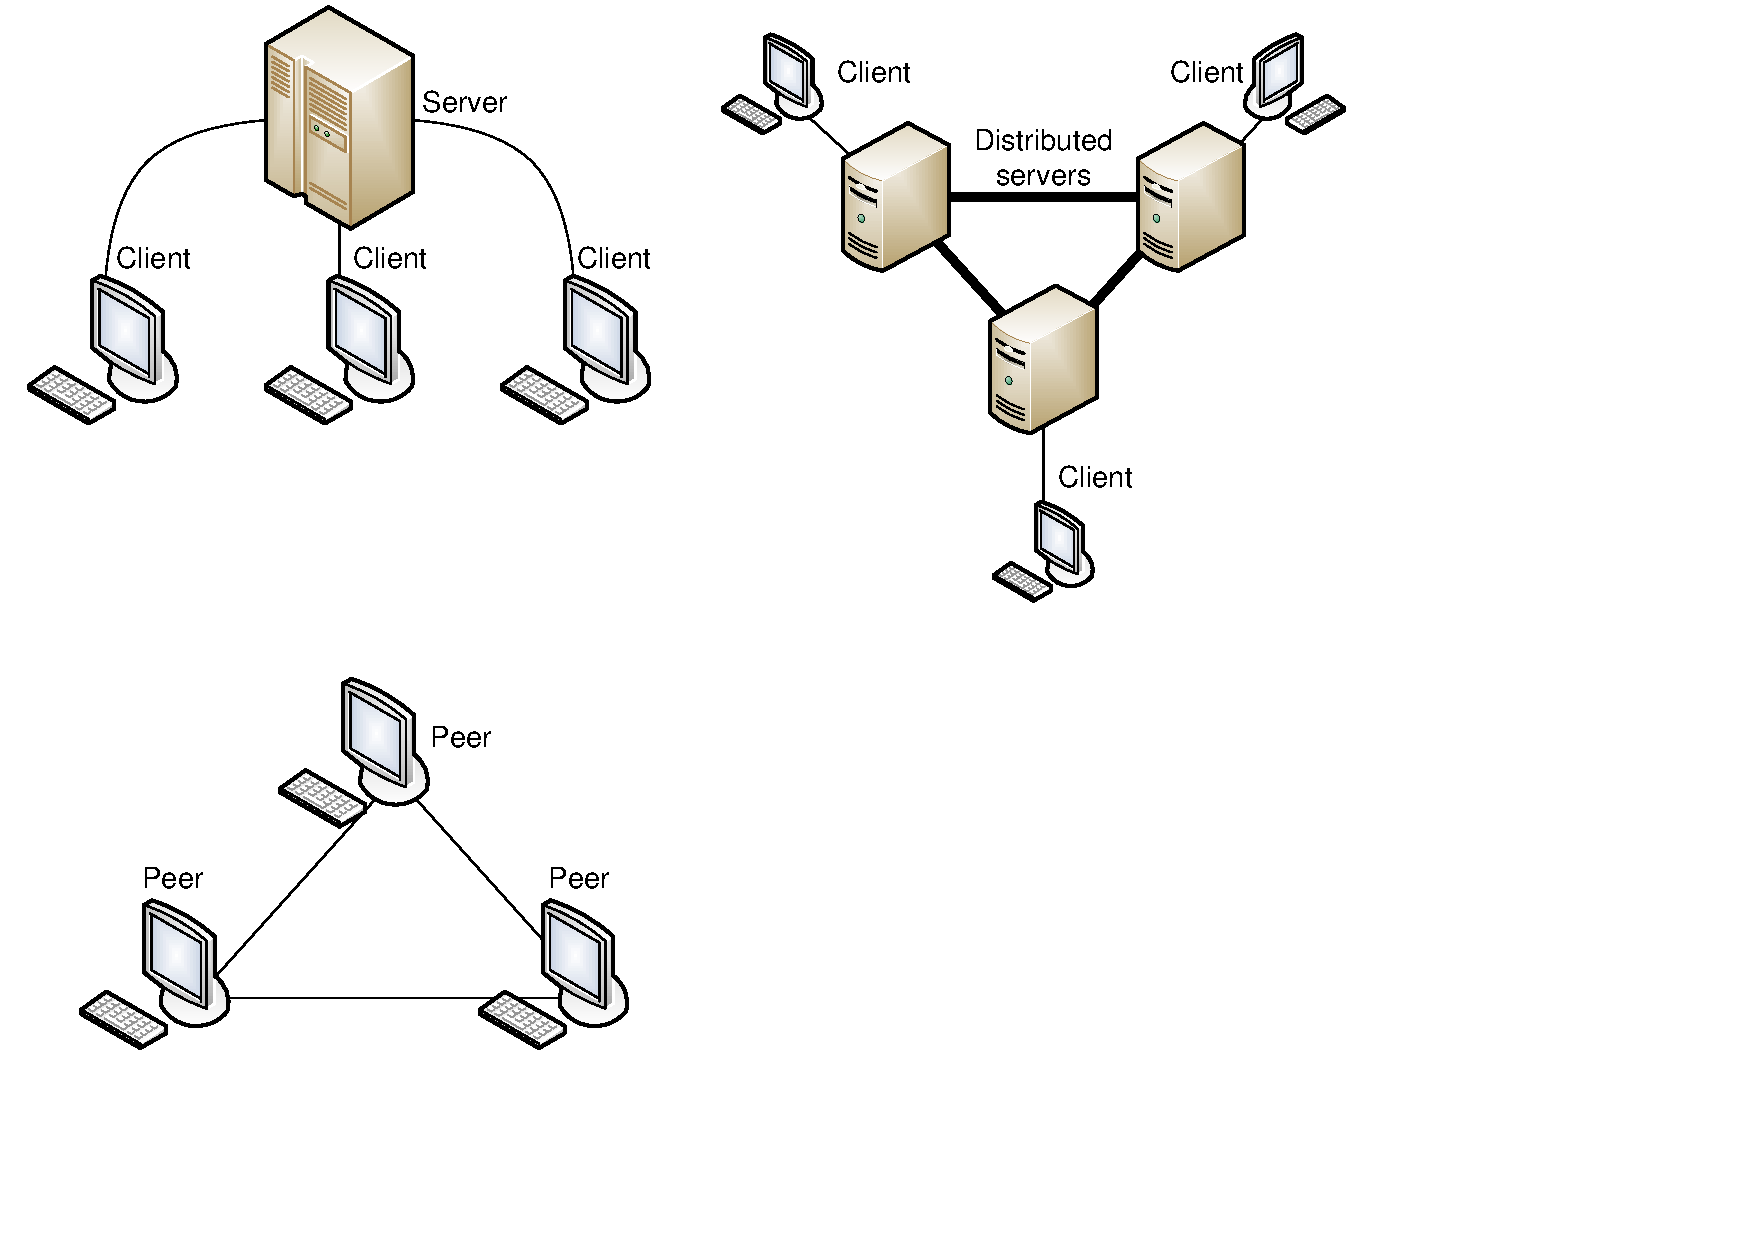
\includegraphics[clip=true, viewport= 0cm 12cm 11.5cm 21.5cm, width=0.5\columnwidth]{network_archs}}
\subfloat[Client/Multi-Server]{\label{fig_cms_arch}
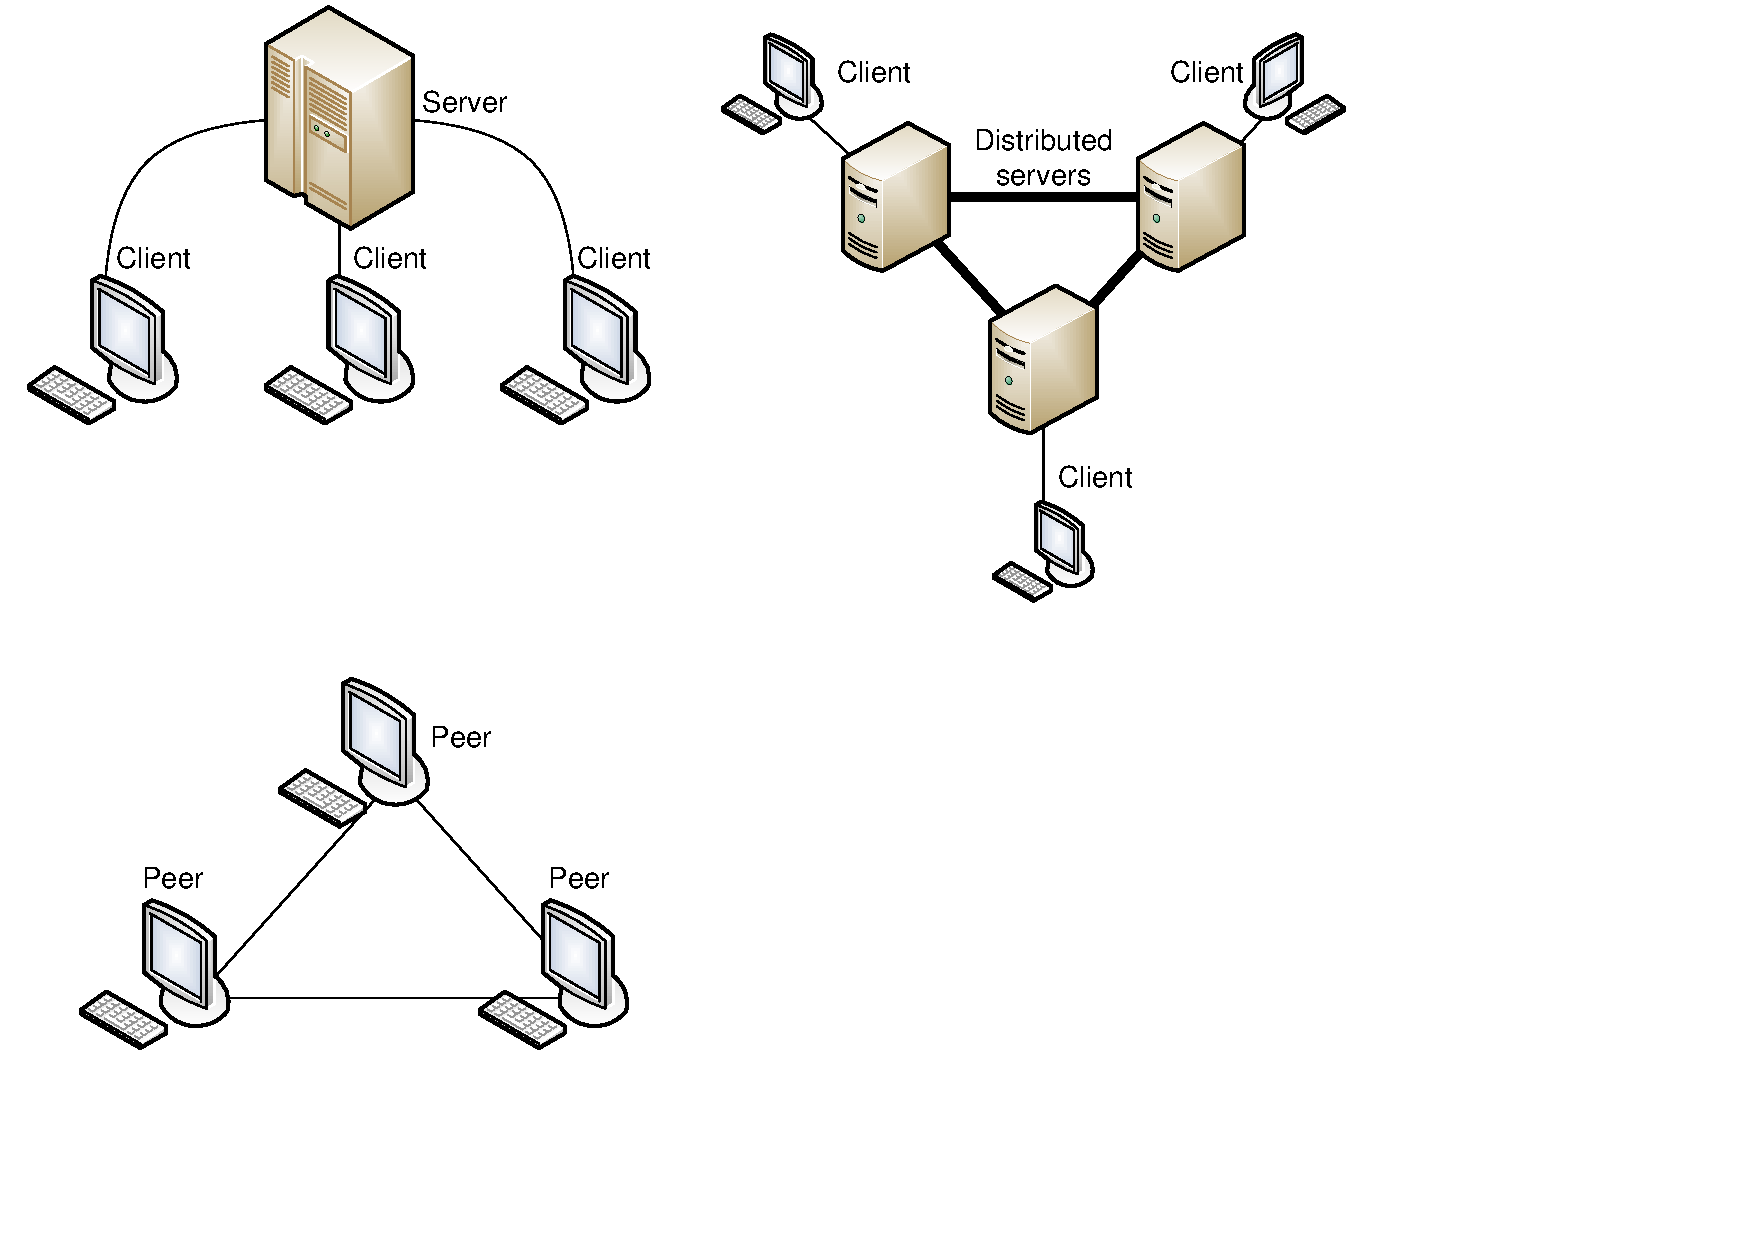
\includegraphics[clip=true, viewport= 12cm 10.5cm 23cm 21cm, width=0.5\columnwidth]{network_archs}}
\caption{Network architectures}
\end{figure}

Figure \ref{fig_cs_arch} shows the C/S model. The server is the entity on which the MMOG is hosted and is controlled by the game operator. Clients are computers operated by players, that connect to the server to play the game. The server is responsible for handling all queries from clients. Clients never communicate with other clients; they send their actions to the server and receive the updated states of other players from the server.

\subsubsection{Advantages}

The C/S architecture has two main advantages that has made it the architecture of choice for all MMOG developers. Because of the centralised approach of the architecture, both administration and security are greatly simplified. Administration is simplified, because the game operator has full control over the server, server data and code. Efficient logging is also supported, because the server is able to not only log all server actions, but also all client actions.

Security is a significant issue in MMOGs, since some players sell in-game currency for real-world currency \cite{chinese_gold_farmer}. This makes the MMOG a platform that is capable of producing income, which increases the incentive of players to gain an unfair advantage over others. The more popular an MMOG, the greater the security threat. Because the operator has full control over the server code and is never required to furnish the
client with the server code, a potential attacker never has any knowledge of the server architecture and code. Because clients are never allowed to communicate, all malicious users can be filtered out of the network by the server when detected and even banned from the network.

Operators are able to ban players, since these games usually require a game account, which is linked to a copy of the game as well as some payment method. This introduces a large cost to players whose accounts are banned. The server or cluster is also housed in a secured location, where access can be controlled. These factors simplify the security of the C/S model by allowing the developers to place all intelligence in the server.

\subsubsection{Disadvantageous}
\label{classic_cs_disadvantages}

The C/S architecture, however, does have some disadvantages. These are: weak robustness, weak scalability, high cost to the operator, high latency, high amount of required server bandwidth and weak handling of transient loads.
\begin{itemize}
\item The robustness of the system is weak because it is a single point of failure. If the server fails or goes down for maintenance, the game is off-line and players are unable to play.

\item The system is also weakly scalable, since a single server cannot easily be extended with more resources. Even if an off-line approach is used, where hardware is upgraded after the system is taken down for maintenance, the hardware required to support a game hosting more than 3000 players, become prohibitively expensive, as described in Section \ref{mmog_cost}.

The server hardware should be able to support peak system loads, which means that sufficient resources should always be provisioned to support these peak load. This is not an economically viable solution, because resources to handle peak loads are not used most of the time. This translates to operators paying for the provisioning of resources, without having active players that pay for these resources.

\item Because no clients are allowed to communicate with other clients, every change that is made to the game world by a client, first had to be communicated to the server, which in turns relays this message to all clients after applying game logic and artificial intelligence (AI) algorithms. This two hop path, with the additional time for computation added by the server as well as possible buffering at the server when many clients communicate, significantly increases the latency of the system compared to a system where direct communication is used.
\end{itemize}

\subsubsection{Client/Multi-Server}

In an effort to address some of the C/S issues, the distributed C/S, also called the Client/Multi-Server (C/MS) model, was introduced, shown in Figure \ref{fig_cms_arch}. In a C/MS model,
the server functions are distributed amongst multiple machines to distribute the server load.

In general, the issues addressed and improved by the C/MS architecture are robustness, scalability, and peak load handling. The system is more robust, because the failure of one server will not necessarily lead to the failure of the whole system for certain system designs. The system is more scalable, because many less powerful servers may be used, which allows for the hosting of more players than what is currently possible with single server hardware. It also handles transient loads better, because, for cases where loads can be predicted, resources can by moved between servers to improve the user experience.

The disadvantages of this system is that the administration complexity is greatly increased. Such systems, although capable of handling many more users than a single server, is also more expensive. These disadvantages are, however, not technical problems and so it is assumed for current games, that these systems are what is required if a game is to be hosted for a large number of players.

\subsection{The cost of doing business}
\label{mmog_cost}

With the fast growing MMOG market, many companies are spending a significant amount of money to produce premium MMOG titles. Some development cost estimates are: \$18 mil. for Aion, \$20 mil., for Everquest \cite{aion_everquest_cost}, \$63 mil. for World of Warcraft \cite{wow_cost} and \$100 mil. to \$200 mil. for Star Wars: The Old Republic \cite{star_wars_cost_1}, \cite{star_wars_cost_2}. Although these figures are purely estimates, it does show that to develop a premium MMOG title costs a lot of money.

The issue with MMOG development is that, although they cost more to develop than single player or smaller scale multiplayer games, they are just as likely to fail. Despite this, game publishers are spending a lot of money in an attempt to recreate the success that is World of Warcraft.

Because of the large revenues being generated from MMOGs, many competitors are entering the MMOG space. Currently, the rate at which new MMOGs are added to the market is outstripping the growth of the market itself \cite{newzoo_mmo_report}. Furthermore, because of the recession, over the past two or three years, game subscriptions have been shown to stabilise or even decline \cite{mmo_growth_chart}.

The significant initial investment required to develop an MMOG also doesn't present the complete picture. Another factor driving up costs for an MMOG is the money required for server hardware, maintenance and support. An MMOG is not finished when it goes live. A team of developers is required to maintain the game, release patches fixing bugs and to produce more content to keep the player base sufficiently interested to ensure that players will continue to pay \$15 per month to play. Development and maintenance costs for World of Warcraft for four years is estimated at \$100 mil. to \$200 mil. \cite{wow_cost}.

With the costs involved, it is therefore difficult for a new developer to enter into this space. After the large initial investment into the game's development, all server hardware must be acquired and staff appointed to maintain the game. This money is spent before it is known whether the game will succeed or fail. It has been estimated that during the lifetime of an MMOG, 80\% of the game revenue goes into hardware and maintenance costs \cite{cs_mmog_cost}.

\subsection{The peer-to-peer proposal}

In 2004, an architecture using the peer-to-peer networking model to host MMVEs was proposed by Knutsson et al. \cite{knutsson_p2p_first}. This
revealed a new research field, which attempts to establish the peer-to-peer (P2P) model as a viable alternative to the classic C/S and C/MS
architectures. P2P MMVE forms the focus of this work. There are various advantages to moving from C/S to P2P in MMVEs. These include: increased robustness, improved scalability, lower operator costs, improved handling of transient player load and lower latencies. The advantages are described in Section \ref{p2p_mmve_advantages} in detail,
but firstly it would be beneficial to acquire a greater understanding of the basics of the P2P network model.

\section{Peer-to-Peer systems}

A P2P network is a distributed network that exists out of many participating nodes to fulfil some objective. In this work, a P2P network is defined as being a distributed network with the following properties
\cite{Rodrigues_acm_comms_p2p}:
%
\begin{itemize}
\item \emph{High degree of decentralisation}:  No or little centralised control exists. Server functionality is distributed amongst all peers.
\item \emph{Self-organisation}: Little or no self-organisation is required in the network. Nodes are given an initial IP to allow them to join the network, but thereafter new neighbours are automatically acquired and nodes remain connected to the network, even with other nodes joining and leaving.
\item \emph{Multiple administrative domains} Peers are not under the control of any single authority. Peers in the network belong to different organisations or individuals and direct administration is impossible.
\end{itemize}

P2P systems have been popularised by mainly three systems developed in 1999: the Napster music sharing service, the Freenet data store and the SETI@home volunteer-based distributed computing project. These three projects highlighted the advantages of P2P networks being: low barrier to entry, scalability, resistance to faults and attacks, and an abundance and availability of resources.

\subsection{The OSI model and P2P overlays}

A basis of computer networking is the layered architecture model, called the open systems interconnection (OSI) model \cite{OSI_protocol_stack}. It defines various protocol layers that allow for abstraction of complex operation in the lower layers in the higher layers. The OSI layers are, from bottom to top: the physical layer, the data link layer, the network layer, the transport layer, the session layer, the presentation layer and the application layer. In practice, the session, presentation and applications layers are usually all folded into the application layer.

The physical layer is the physical transmission medium and carries physical signals. Physical level protocol standards include: IEEE 802.11 (Wi-fi), USB, Bluetooth, etc.. The data link layer, sometimes referred to as the MAC layer in the Internet protocol stack, carries frames and is responsible for point-to-point data transfer on the same local area network (LAN). Signals from the bottom layer are converted into bits and sequences of bits are grouped into frames, which is seen to be sent over the data link layer. As can be seen, every higher layer abstracts elements of the lower layer to reduce complexity.

The network layer allows communication between different LANs, using routers, gateways and host addressing. Every computer in a network is referred to as a host. A well known network layer protocol is the Internet protocol (IP), which routes all Internet traffic. The transport layer is referred to as the end-to-end layer and represents the abstract connection between a source and destination host, where all intermediate routers and LANs may be ignored, since they are abstracted away by the network layer. Well known protocols in this layer include the user datagram protocol (UDP) and transport control (TCP) protocol. Above the transport layer, for the purposes of this work, is the application layer. The application layer has access to all network services, including routing and reliable transmission.

In the C/S architecture, the client and server are both located in the application layer and communicate with each other using the transport layer. They need not be aware of any of the lower layers.

P2P networks are created and maintained in the application layer of the OSI model, called the P2P overlay. An overlay is required so peers may know which other peers are part of the P2P network, since most nodes on the Internet will not be part of the network. The overlay is then defined by the routing table information stored on each peer. The overlay can be thought of as an additional layer in the OSI model. The overlay interfaces with the transport layer and P2P applications are one layer higher and communicate by using the overlay.

Peers in an overlay network might have neighbours that have no relationship to their physical position in the underlying network.

\subsection{Structured and unstructured P2P overlays}
\label{overlays}

Overlays can broadly be classified into structured and unstructured types. The classification is mostly based on the differing methods of routing and content retrieval in the network. This section only provides a brief comparison between structured and unstructured overlays. For a detailed comparison between the two types that also deals with many of the myths of structured overlays, please refer to \cite{Castro_structured_overlay_myths}.

With unstructured approaches, one is never assured that a data item will be retrieved, even if that data item is present in the network. If many duplicates of a data item are contained in the network, this becomes less of a problem, since it is assumed that the request will be routed to some set of nodes that do  possess the item.

An unstructured architecture is well suited to content sharing and Voice over Internet Protocol (VoIP) networks, for example: P2P TV, BitTorrent, Gnutella and Skype. The reason for this is the high level of duplication in these networks, especially for popular content. It is also easier to perform keyword searches in unstructured networks and the overlay requires less maintenance.

Structured overlays have been proposed that provide for efficient routing and reliable retrieval of data items. Some of these well known overlays are: CAN \cite{CAN}, Chord \cite{chord}, Tapestry \cite{tapestry} and Pastry \cite{pastry}. The basic principle of a structured overlay is that all nodes are identified by unique identifiers (IDs).

A popular method to create the IDs is to use hashes to a circular key space, using for example, the SHA-1 hash function. Any node in the overlay network is then able to efficiently route a query with a given ID, to a node with an ID closest to the given ID. An accurate comparison is that unstructured overlays are good at finding ``hay'', while structured overlays are good at finding ``needles'' \cite{Rodrigues_acm_comms_p2p}.

\subsection{Features of structured P2P overlays}

A structured P2P overlay has certain key features that determines its lookup speed, space consumption and bandwidth requirement \cite{p2p_networking_handbook}. These features are geometries, routing algorithms, join/leave mechanisms, routing table maintenance and bootstrapping.

\subsubsection{Geometries}

An overlay's geometry determines how nodes are structured in the application layer network. The geometry allows for deterministic routing. The geometry determines the number of required lookup hops and how the network will be maintained during times when nodes join and leave the network, called churn.

\subsubsection{Routing algorithms}

The routing algorithm is directly related to the specific overlay geometry. The routing algorithm determines which nodes are traversed when a message is sent to a target node. The routing algorithm and the geometry determines the number of expected hops for a message to reach a destination.

\subsubsection{Join mechanism}

P2P networks experience constant churn, where nodes are joining and leaving the network. Mechanisms for a node to join the network should be present. This is usually in the form of a well known directory (boostrap) server. When a node wishes to join the network, the directory server sends a set of nodes that the node may want to join.

\subsubsection{Leave mechanism}

If a node leaves the overlay, its neighbours have to be informed so they may update their routing tables. This is termed \emph{routing table maintenance} and has to happen every time a peer leaves the network. Neighbouring nodes of a node that left the network might also have to inform their neighbours of the change. Two types of routing table maintenance exist: opportunistic and active maintenance.

Opportunistic maintenance attaches routing information to existing request packets. Routing data is essentially ``piggy backed'' onto existing messages. This reduced messages overhead but the rate of routing table maintenance is directly proportional to the message rate. Active maintenance makes use of explicit update messages, which required more bandwidth but is more reliable.


\subsubsection{Bootstrapping}

After having been informed of a peer to join, a joining peer may initiate the process of positioning itself in the P2P network, called bootstrapping. This is the process of finding out where the joining node fits into the overlay in terms of the geometry. If the overlay requires that all nodes be connected in a ring organised by ID, then the joining peer must discover the nodes whose IDs are one more and one less than its own and join those two peers.

The process of bootstrapping is complete when a joining peer becomes a functioning member of the P2P overlay.

%TODO: Add something about the effect of the hashing and why it's important

\subsection{Advantages}

\begin{itemize}
\item P2P networks have a low barrier to entry, since little or no centralised infrastructure is required to maintain the system. This makes P2P networks inexpensive to operate and is one of the reasons Napster was able to provide its service for free.

\item P2P networks are considered scalable. Pure P2P networks can theoretically grow from hundreds to millions of nodes, with the service remaining functional. This is all possible without the need for the operator to acquire more infrastructure, as opposed to the centralised client/server network, which required more powerful server clusters are the network grows to handle the growing number of client requests.

\item A P2P network is also resistant to faults and attacks, since the failure of a single node has little to no effect on the network. This is because there are usually few nodes that are critical to the correct functionality of the system. To incapacitate a P2P network, an attacker usually has to shut down a large proportion of the network.

\item Not only does a P2P operator not require its own infrastructure, but the P2P infrastructure that forms part of the network and consists of peer machines provide abundant and highly available resources, being computation power, long term and short term storage. This means that P2P networks can be designed to run on powerful computers.
\end{itemize}


\section{Peer-to-Peer MMVE network architectures}
\label{p2p_network_architectures}

P2P MMOGs are considered a sub-class of P2P Massively Multi-user Virtual Environments (MMVEs), a class that also includes large scale military simulators.

This architecture does, however, still have a few major issues that need to be solved before MMVEs can be developed that use it. If
these issues, discussed in Section \ref{key_challenges}, can be solved, a P2P architecture holds some powerful advantages over a C/S system.

The core idea of the P2P model is that each peer contributes sufficient resources to the network to host itself. This also means that all functions of the server in the classic C/S model are distributed amongst all peers.

\subsection{Advantages}
\label{p2p_mmve_advantages}

\begin{itemize}
\item The P2P architecture is robust, because there is no server that can fail, only individual peers. Individual peers failing will not affect any other peers other than the peer that failed. This behaviour makes game down-time extremely unlikely.

\item The system is scalable, because every peer hosts itself.

\item Because of the high scalability, no extra resources are required from an operator perspective, when more peers join the network.

\item P2P networks also efficiently handle transient loads, since the joining peers contribute their own resources. If many players suddenly enter the
game no resource provisioning issues will arise, since peers already possess the required resources.

\item P2P architectures create a lot of opportunities for independent developers, because a large initial investment is no longer required to purchase
the expensive server hardware. Not only are hardware costs reduced, but running costs are also reduced.

\item Bandwidth required by the game server is now shared amongst users, which means that very little bandwidth costs will be incurred by the provider.

\item Latency is improved, because it is now possible to directly communicate between peers and it is not necessary to communicate via a server.
The distribution of the load as well as direct communication will further reduce latency.
\end{itemize}

\subsection{Requirements}

Key requirements have been identified for the creation of a P2P MMVE. What follows is an expansion and reinterpretation of the requirements identified by Schiele et al. \cite{Schiele_p2p_requirements}.

\subsubsection{Distributed computation}
\ref{distributed_computation_requirement}

Non-Player Characters (NPCs) are characters that are not controlled by any human player, but are rather controlled by some artificial intelligence routine or script executing on some host machine. These characters represent the traders and monsters in MMVEs and usually contain sets of rules that determine how they should interact with Player Characters (PCs) as well as their own state information. An NPC's state can be how much money and items it has to trade or how much health it still has after being attacked by a player.

Some game objects require computational power to function. An example of this is the Artificial Intelligence routines of NPCs or the computation of physics effects on in-game objects. In P2P MMVE, it might be required to distribute these computational tasks to offload computation load from peers that do not have sufficient resources.

\subsubsection{Consistency}
A key challenge with any networked game is how to maintain state consistency between users in the virtual world. In other words, to ensure that all users perceive a virtual world in the same state. Solving the state consistency problem for P2P MMVEs is one of the major development challenges and forms the focus of this work. The challenge of state consistency will be described in detail in Chapter \ref{chp:CONSISTENCY}.

\subsubsection{Persistency and state management}

\subsubsection{Self-organisation}\
Handling of user churn

\subsubsection{Availability}
Game must always be online (P2P requirement)

\subsubsection{Interactivity}
Low latency interaction and masking latency with dead reckoning

\subsubsection{Scalability}
Server and peer bandwidth requirements

\subsubsection{Security}

Security, which includes cheating mitigation, has been identified as a major issue for P2P networks \cite{knutsson_p2p_first}, \cite{challenges_p2p_gaming}, \cite{cheat_proof_event_ordering}. The challenges reside in the fact that peers are not under the control of the game producer. Since all server data are distributed amongst peers, all peers have access to sections of the server data. Peers also have access to the distributed server code. One advantage that can be exploited to prevent cheating is that no peer contains all server data and no single peer has more authority than another.

\subsubsection{Efficiency}
The peer must efficiently implement the server, since it still has to be a client as well

\subsubsection{Maintainability}

\subsubsection{Incentives}

P2P schemes require all players to share resources in order to ensure correct functionality. Players might, however, not want to share their resources, whilst still benefiting from the resources of others. The purpose of incentive mechanisms is to ensure that all players contribute resources, by incentivised contribution.

All distributed resource sharing models require incentive mechanisms. For example, Bittorrent systems use the tit-for-tat protocol to ensure that all people downloading data are also contributing data \cite{tit_for_tat}. Such mechanisms are also required with P2P MMVEs. One advantage in designing an incentive mechanism for a P2P MMVE is that players can be made to contribute resources for the duration of play. The issues with file sharing systems are not present where a peer, after downloading a file, has no more incentive to contribute.

\subsubsection{Structured P2P overlay}

Because there is no assurance that a data item might be retrieved from an unstructured network, especially when that item is scarce, unstructured overlays are not considered adequate as a basis for P2P MMVEs, where all data items must be available at all times.

A P2P MMVE architecture requires a structured P2P overlay in the broad sense. In P2P MMVEs, peers have to be connected in some geometry and it should be possible to route messages between peers. P2P MMVEs require a bootstrapping server to enable peers to join the network and be placed in it. A P2P MMVE architecture should handle churn with a minor impact on system operation. Most importantly, all objects stored in the P2P MMVE should be available at all times.

\subsection{Key challenges}
\label{key_challenges}

Using P2P MMVEs has many advantages, some challenges still remain. The main challenges are state consistency, limited peer bandwidth, cheating mitigation, incentive mechanisms and distributed computation. This section will present some information on work that has been done in the different areas and talk about the maturity of the various solutions. In general though, most solutions are still research projects and none have yet been implemented as commercial products.

\subsubsection{Peer bandwidth}

In a paper by Miller and Crowcroft, a packet simulator was created to determine the required bandwidth and effective latency, if a game such as World of Warcraft were to be implemented using P2P technologies \cite{Miller_p2p_infeasability}. Their simulation results indicate that today's networks are not able to host P2P MMVEs, with the required bandwidth and latency constraints. Such a significant result requires verification, but at the least, it shows that reducing bandwidth and latencies for P2P MMVEs should be a primary design requirement.

\subsubsection{Cheating mitigation}
\label{key_challenges_cheating}

%Describe "server data" in terms of a more generic form to be able to have that generic form in the server and p2p architecture.

There are various security issues that are usually classified according to the level in the OSI protocol stack where they occur. The areas identified by \cite{cheat_proof_event_ordering} and expanded upon by \cite{cheating_taxonomy} are: game level, application level, protocol level and infrastructure level. The description is consistent with the generally used layered security model \cite{distributed_systems_security}.

\begin{itemize}
\item Game level cheats are ways in which a malicious player may gain an unfair advantage over other players, within the confines of the game. These cheats are usually because of software bugs and some examples are duplication and teleport cheats.

\item Application level cheats are where malicious players alter the game software to gain an unfair advantage. This is usually done by gaining access to the game state to which they should not have access at the current time. An example of this is ``map reveal'' cheats in strategy games, where the ``fog of war'' is removed and the player can observe all the opponent's movements. Other cheats that are used include augmenting the player's UI with extra information that allows the player to make more informed decisions.

\item Protocol level cheats are cheats based on the different methods of communicating data across the system. These usually concern dropping, delaying of modifying IP packets to achieve certain outcomes in the game.

\item Infrastructure level cheats concern exploiting the underlying infrastructure on which a game is built. Types of infrastructure cheats include denial of service (DOS) attacks on the P2P overlay to prevent messages that should be forwarded by a peer from being forwarded.
\end{itemize}

As with all taxonomies, all cheats may not cleanly fit into one if these boxes, some cheats may occur over multiple levels or a cheat with a specific outcome can be implemented differently on different levels. The field of P2P security has recently received more attention than in the past and has started to bear fruit \cite{survey_p2p_game_cheats}.

This is, however, an ongoing research field with many issues still open. For an in-depth review of the security issues facing peer-to-peer system in general, refer to \cite{p2p_security_issues}. These issues are the same issues facing P2P MMVEs, with the exception of the game and application layer issues.

\subsubsection{Incentive mechanisms}

Some proposed incentive schemes increase a player's reputation when resources are provided  \cite{classic_p2p_reputation} \cite{proactive_reputation}. This might create a type of meta game, where players try to gain as much reputation as possible. It can however be argued that this scheme does not really enforce the provisioning of resources. A player who does not want to provide resources might not see a higher reputation as sufficient incentive to provide resources.

Other issues with incentive schemes is that sometimes players might have insufficient resources. Such players should be aided by other players with sufficient resources and not be disallowed from playing the game. When limited resources are taken into account, the issue of reporting a false amount of available resources becomes a problem. A peer that has sufficient resources, might report insufficient resources, to avoid being penalised. It is evident that there is a need for more research in this field.

\subsubsection{Distributed computation}

Some architectures assume that the computational requirements will be fulfilled where the object state is hosted \cite{solipsis}, but other schemes exist that allow for the CPU power to be distributed amongst peers. One such scheme makes use of a ``job board'' like mechanism, where tasks are advertised on specialised peers. All peers monitor these specialised peers and may elect to perform the advertised tasks \cite{fan_mediator_paper}.

\subsubsection{State consistency}

The state of the art of state consistency techniques will be reviewed in detail in Chapters \ref{chp:CONSISTENCY} and \ref{p2p_MMVE_state_persistency}.

\section{Research objectives}

\section{Related work}

\section{Contributions}
\label{objectives}

\begin{itemize}
\item A generic state consistency model is developed that encompasses both C/S and P2P consistency models.

\item A review of various state management and state persistency systems is performed.
    \begin{itemize}
    \item The state management survey identifies some key metrics by which state management systems may be compared.
    \end{itemize}

\item A novel state management and persistency architecture, called Pithos, is proposed and implemented in simulation, which increases reliability and responsiveness compared to classic state persistency methods.
    \begin{itemize}
    \item Multiple methods of implementation are described that provide different benefits, depending on the situation.
    \item The various implementation methods are evaluated and recommendations are made on which methods work better in which situations.
    \end{itemize}

\item A statistical model for expected object lifetimes is developed and used to verify the Pithos results.
\end{itemize}

\begin{itemize}
\item Early in the literature study phase, it was discovered that no research projects that deal with P2P MMVEs present the complete picture of the field. A significant amount of research has been done in the field of state consistency (reviewed in Chapter \ref{chp:CONSISTENCY}), but in this field, no model has been provided which shows what is required to build a complete state consistency architecture. The first contribution of this work is to provide such an architecture at the start of Chapter \ref{chp:CONSISTENCY}.

\item The generic consistency model that is developed is not only applicable to P2P MMVEs, but to any networked virtual environment that required state consistency. The generic consistency model is also compared with well known client/server and P2P consistency models, to show how the existing models can be seen as more specialised versions of the generic consistency model.

\item After developing a generic consistency model, this work then focusses on an area of state consistency that has received little attention from the research community, namely: state management and state persistency. This area is concerned with managing object states as they are updated by events occurring in the virtual environment. Also during a literature review of this field, it was found that no thorough review of this field has been done to compare the different types of storage systems present in P2P MMVEs and presented in the literature. We then preceded to perform such a review, presented in Chapter \ref{p2p_MMVE_state_persistency}. The results of this survey has also been published in the IEEE Transactions of Parallel and Distributed Systems \cite{gilmore_p2p_mmog_state_persistency}.

\item During the survey, some key metrics were identified by which state management and state persistency systems may be described. A proposal was also made as to how these metrics may be measured. What was found upon completion of the survey is that no storage system has thus far been created to satisfy all identified metrics. Work was then undertaken to develop a novel state management and persistency architecture that satisfies all identified requirements.

\item The state management and persistency architecture has been developed and called ``Pithos''. Pithos has been implemented in a network simulation framework, called Oversim, which runs on the Omnet++ simulation environment. The Oversim framework itself has also been extended to implement our novel generic consistency architecture. Pithos has been implemented in the root object store section of this architecture.

\item Many of the key mechanisms in Pithos, such as object retrieval, have been implemented using multiple methods. These methods are then compared to determine the advantages and disadvantages of each. Pithos is also compared to the storage systems identified. Pithos always shows similar or improved performance over classic storage systems in all identified areas.

\item In order to verify the correct functioning of Pithos, mathematical models are also developed to describe Pithos's performance in the various identified metrics. Amongst these is a novel Mathematical model that makes use of an embedded continuous time Markov chain to determine expected object lifetime for varying amounts of network churn, various network sizes and replication rate. The mathematical model is compared with actual Pithos results and appears to match almost exactly.
\end{itemize}

\section{Summary of this work}

Chapter \ref{chp:CONSISTENCY} presents an overview of state consistency models. Initially, it describes the general process by which state consistency is achieved. Some classic consistency models are then presented in terms of the generic model. Consistency models for P2P MMVEs are then presented, with an overview of work that has been done in each of the various sections required to implement a complete consistency model.

Chapter \ref{p2p_MMVE_state_persistency} focuses on the state management and state persistency aspect of P2P MMVE state consistency. Initially, some metrics are defined according to which different storage architecture may be compared. A literature review is then presented, where papers that deal with various storage techniques are grouped and the advantages and disadvantages of each group is then discussed. This chapter also identifies a need for a novel state management and persistency architecture.

Chapter \ref{chp:DESIGN} describes the design and implementation of Pithos, the novel state management and persistency architecture. Initially, the overarching Pithos design is described, including the perceived use case and design goals. The Oversim simulation environment is then described, along with the extensions that were made to model the generic consistency model. The Pithos implementation is then described in terms of Oversim modules. Key mechanisms that implement that Pithos design are then presented with reference to the Pithos Oversim modules. Various methods to implement some mechanisms are descried.

Chapter \ref{chp:EVALUATION} evaluates the Pithos implementation. The performance of the key mechanisms are presented and the various implementation methods are compared. Pithos is also compared with other storage implementations.

Chapter \ref{chp:MODELLING} models Pithos's performance with reference to the identified metrics for P2P MMVE storage systems. A focus is placed on expected object lifetime and a novel model is developed, based on an embedded continuous time Markov chain.

Chapter \ref{chp:VERIFICATION} compares model results with Pithos simulation results. The purpose of this chapter is to verify the correct functionality of Pithos, according to mathematical models. The chapter also explores how to design storage systems with desired object lifetimes.

Chapter \ref{chp:CONC} concludes the work. It presents a summary of the work, lists contributions made and discusses some future areas of research.

\chapter{State Consistency}
\label{chp:CONSISTENCY}

Key to designing an MMVE is to design its state consistency architecture. On a physical level, each computer that executes a virtual environment (VE) is executing a copy of the virtual environment. This is because a computer can only operate on what is stored in its primary memory. Because computers cannot access each other's primary memory banks, the necessity of multiple object copies is created.

A virtual environment can be characterised by its state. The \emph{environment state} (\emph{game state} when the environment is an online game) includes all positions, health and other attributes of all avatars, NPCs and other objects in the VE. The environment state consists of a collection of objects. An NPC as well as an immutable plant are both examples of objects that together make up the environment state.

When discussing how to segment VE state, it is sometimes easier to speak in terms of \emph{objects}, since they are separable. For the purposes of this work, objects are entities with both state and logic, which means they consume both storage space, as well as computing resources. Objects can also produce events, which should be sent to other objects. When this definition is used, NPC objects may be classified as a specific type of object, which forms part of the global game state.

The existence of multiple object copies necessitates an object consistency model. In MMVEs, each computer uses the information of the virtual environment, stored in memory, to display the virtual environment to the user. The user makes decisions based on what is displayed and the executed operations on the environment. These operations can effect change in the environment and this change has to be communicated to all other entities capable of interacting with the environment. The fact that users operate on a local version of the environment and that the environment should appear the same to all users requires state consistency mechanisms.

\section{Event-logic-update cycle}
\label{event_logic_update}

It is however impossible for multiple object states to always be consistent, because it takes time to send a message about an object update that has occurred. It is, therefore, not a good design to allow objects to be locally changed and those changes to then be communicated to other objects, because other objects may also have been locally changed in a way that would not allow for the change in the first object.

An example would be of one player in a virtual game world dealing five damage to another player with five health. When the damage is dealt, the target player is killed. If, however, the player drank a potion that gives it some health, the damage dealt by the first player would not kill him. The state of the player being dead and the player being alive is not possible at the same time.

To overcome this difficulty, a disconnect is introduced between the actions that can be performed on objects and the effect that the actions can have on objects. This is called the event-logic-update cycle \cite{}.

\emph{Events} are generated by objects and can be thought of as actions taken by agents, where agents can be humans or artificial intelligence (AI) scripts. These include casting a spell, using an item or walking.

\emph{Environment logic} is applied to events to determine what updates should be applied to the environment state. Environment logic is thus a ``think'' function, which determines how the environment should change as a result of an event. Another way to think about environment logic is to see it as the game rules.

A player casting a spell might cause another player's health to be reduced, her own health to be increased or a monster to spawn. When a player is walking, the logic will cause the player's position to update at the player's walking speed.

Environment logic communicates how the world should change via \emph{state updates}. State updates are the incremental changes that specify how the environment state should change.

An object exists in two forms: the authoritative object and the non-authoritative object. The state of the authoritative object is considered to be the true state or absolute state. Copies of the authoritative object can be made, but these copies are all non-authoritative objects. If a discrepancy occurs between an authoritative object and a non-authoritative object, the state of the authoritative object is considered to be the true state. The work of the consistency mechanism in the VE is to ensure that all non-authoritative object states follows the authoritative object state within a time frame that is reasonable for the particular VE and the particular type of object.

Authoritative objects are the objects traditionally housed on the server in the C/S based MMOGs. All clients obtain replicas of these objects and duplicate them locally in order to perform low latency computations. An example would be an NPC monster. When players perceive the monster in the virtual world, a duplicate of the NPC objects is sent to the user's computer for display purposes. When another player attacks the NPC, the change in health will be computed at the server and an update is then sent in order to ensure consistency between root and replica objects.

\begin{figure}[htbp]
 \centering
 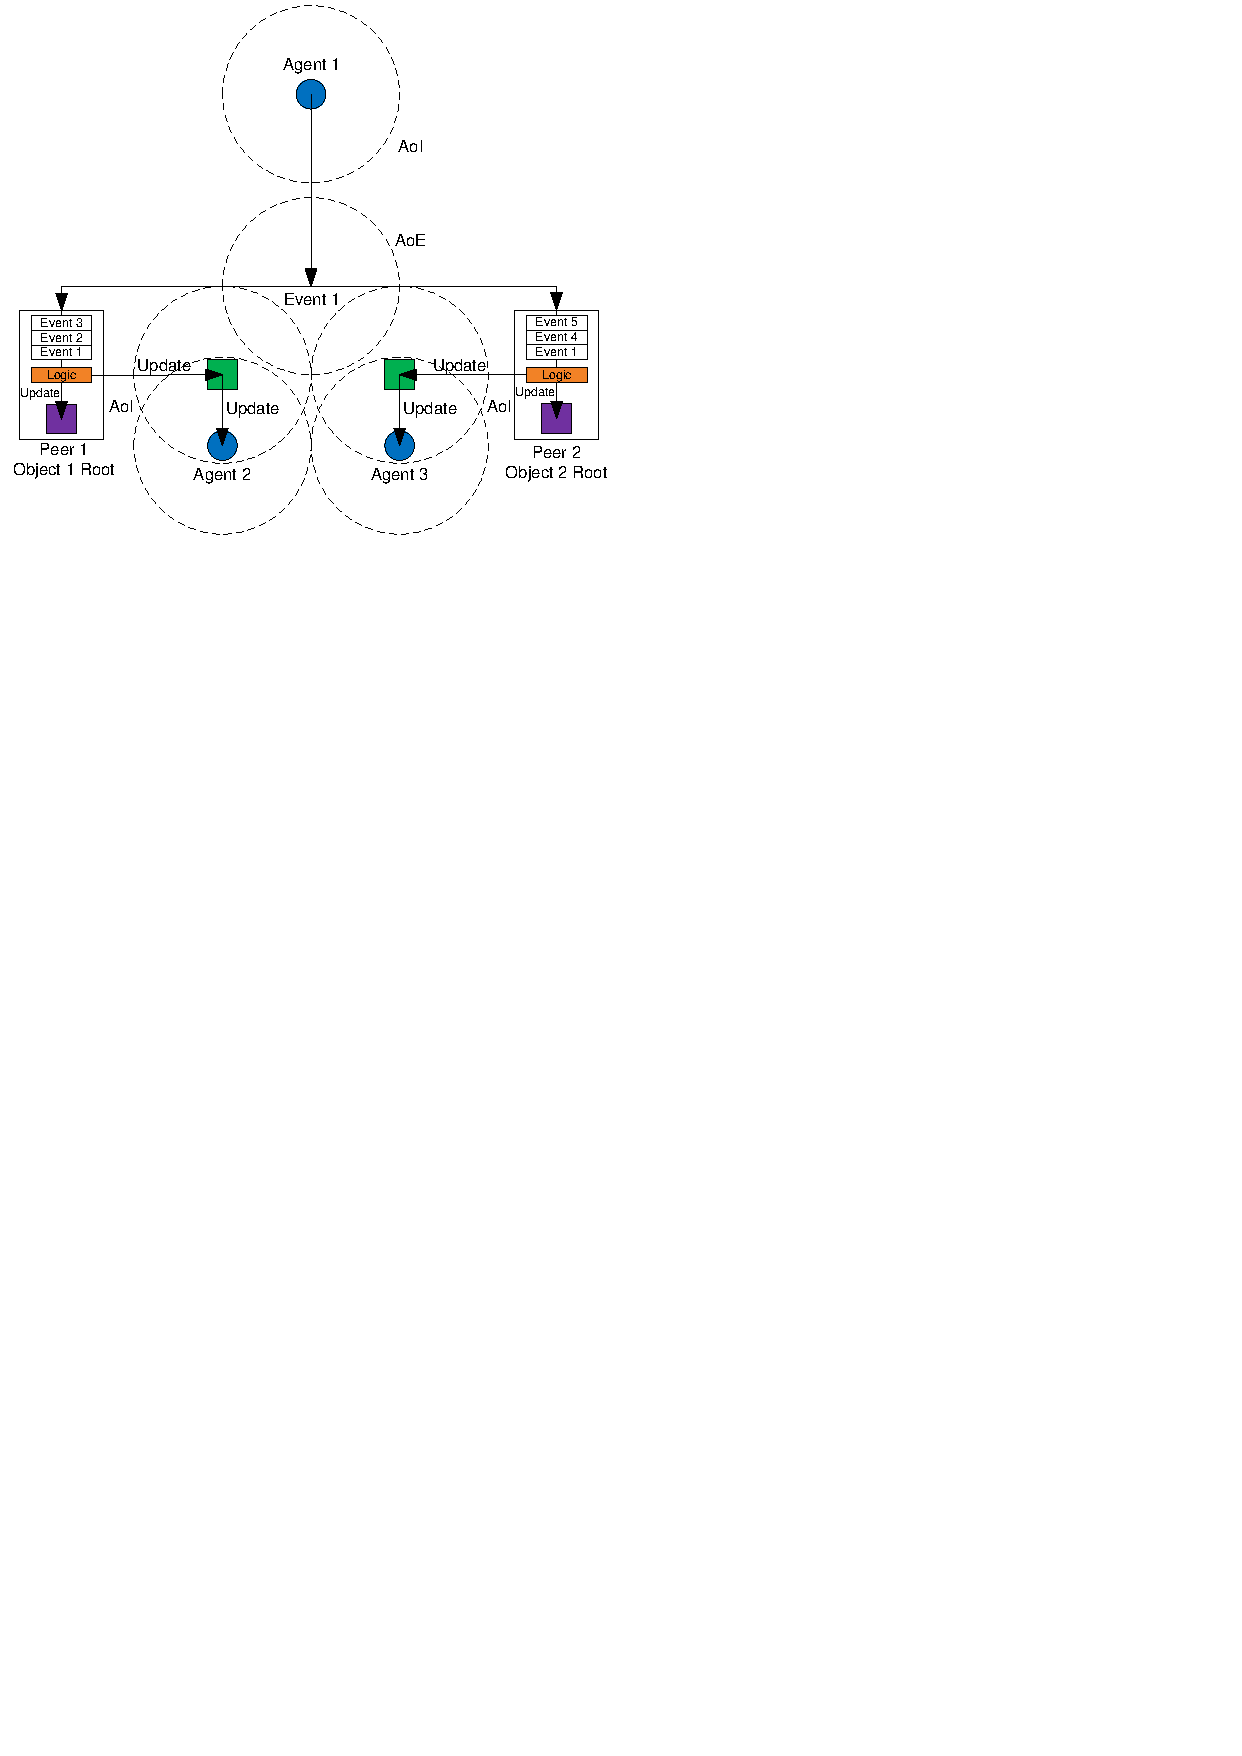
\includegraphics[clip=true, viewport=0cm 20.5cm 10.5cm 30cm, width=0.8\textwidth]{generic_consistency_graphic}
 \caption{Graphic showing the flow of events and updates to achieve state consistency}
 \label{fig_event_update_flow_graphic}
\end{figure}



\section{Classic consistency models}
\label{classic_models}

As an introduction to consistency models, an overview of the two common models, currently used in computer games will be described. The models used
in P2P MMOGs are all permutations of these two basic models. The two models are based on the two different network models. These are the fully
distributed model, also called the event-based model \cite{p2p_cm_aoe}, and the C/S-based model, also called update-based model
\cite{unreal_networking}.

\subsection{Event-based (Fully distributed)} \label{classic_cs_event_based}

\begin{figure}[htbp]
\centering \subfloat[Event-based (fully distributed)]{\label{fig_p2p_cm}
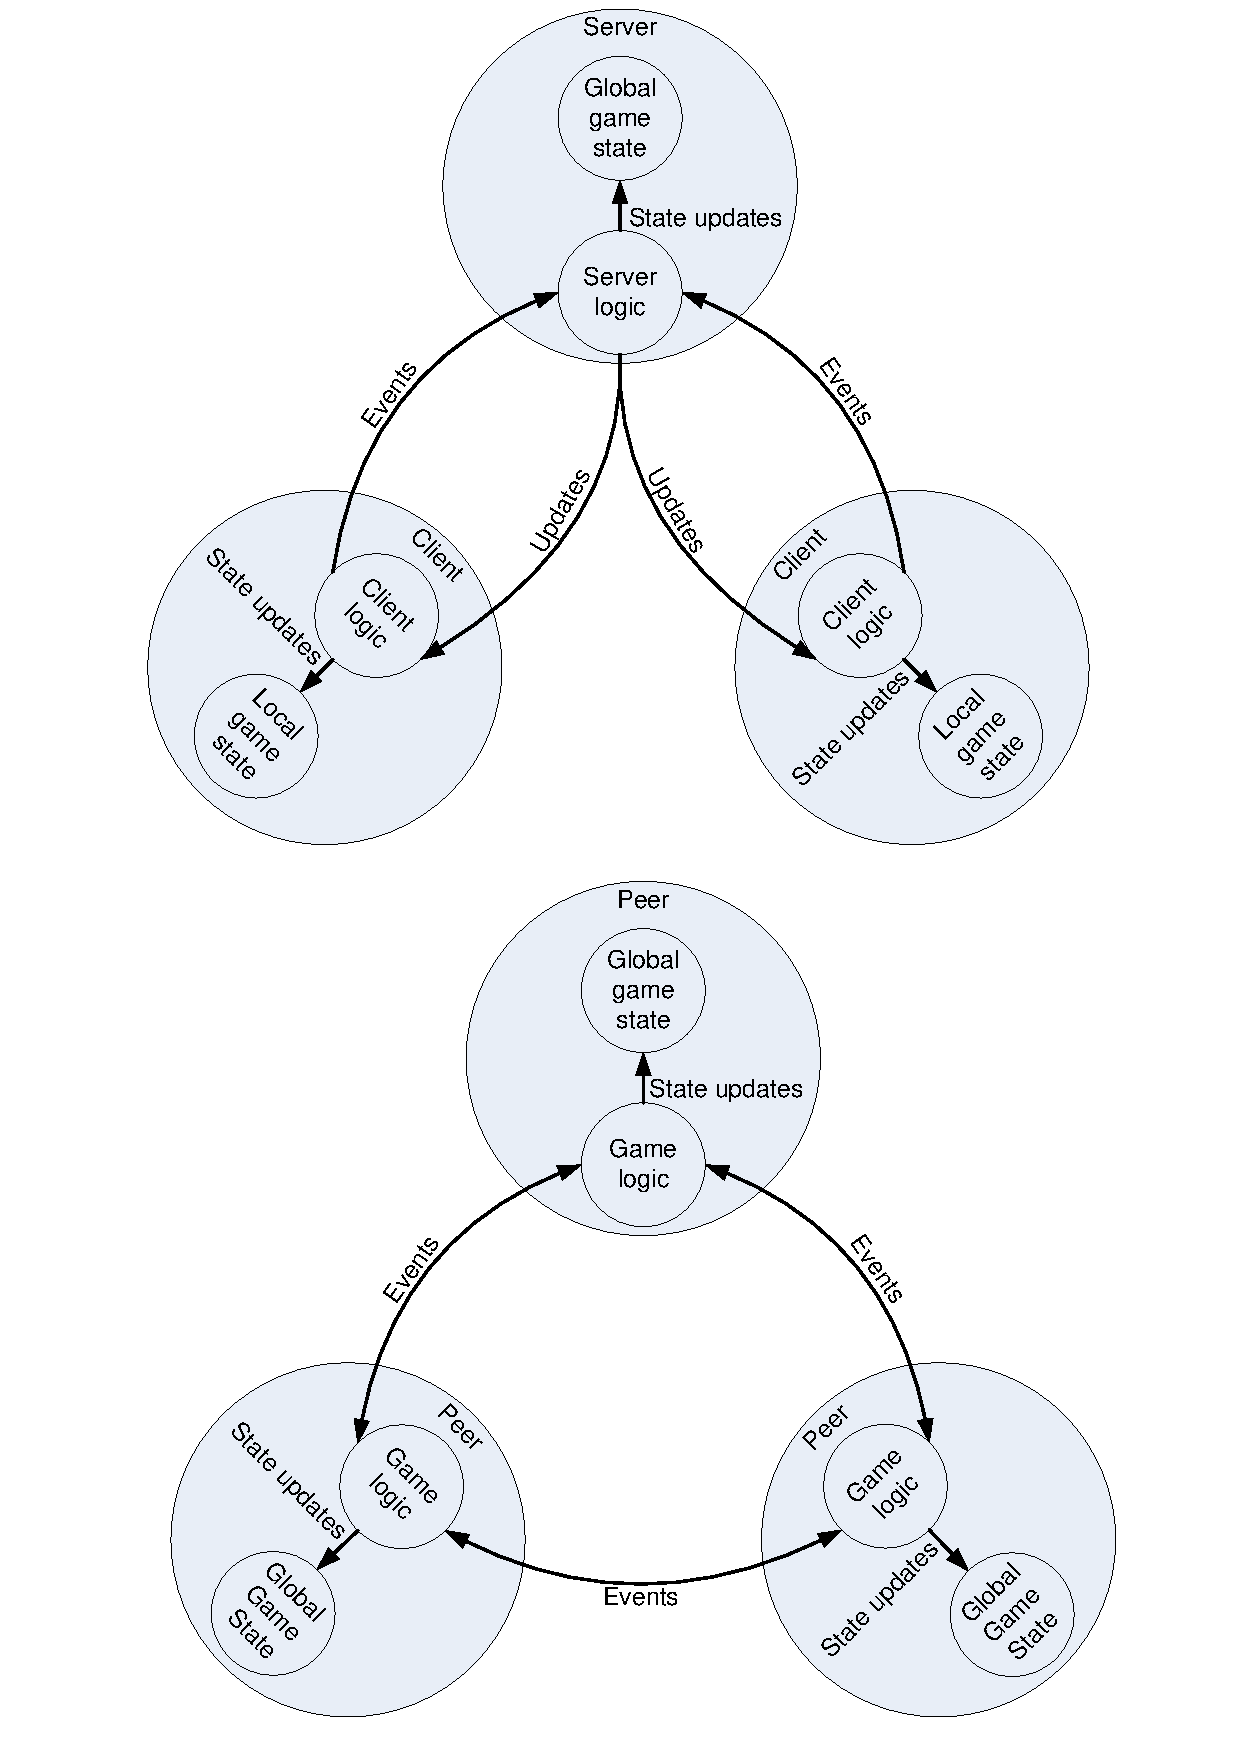
\includegraphics[clip=true, viewport= 2.5cm 0.5cm 19cm 15cm, width=\columnwidth]{CS_P2P_CMs}}
 \subfloat[Update-based (client/server)]{\label{fig_cs_cm}
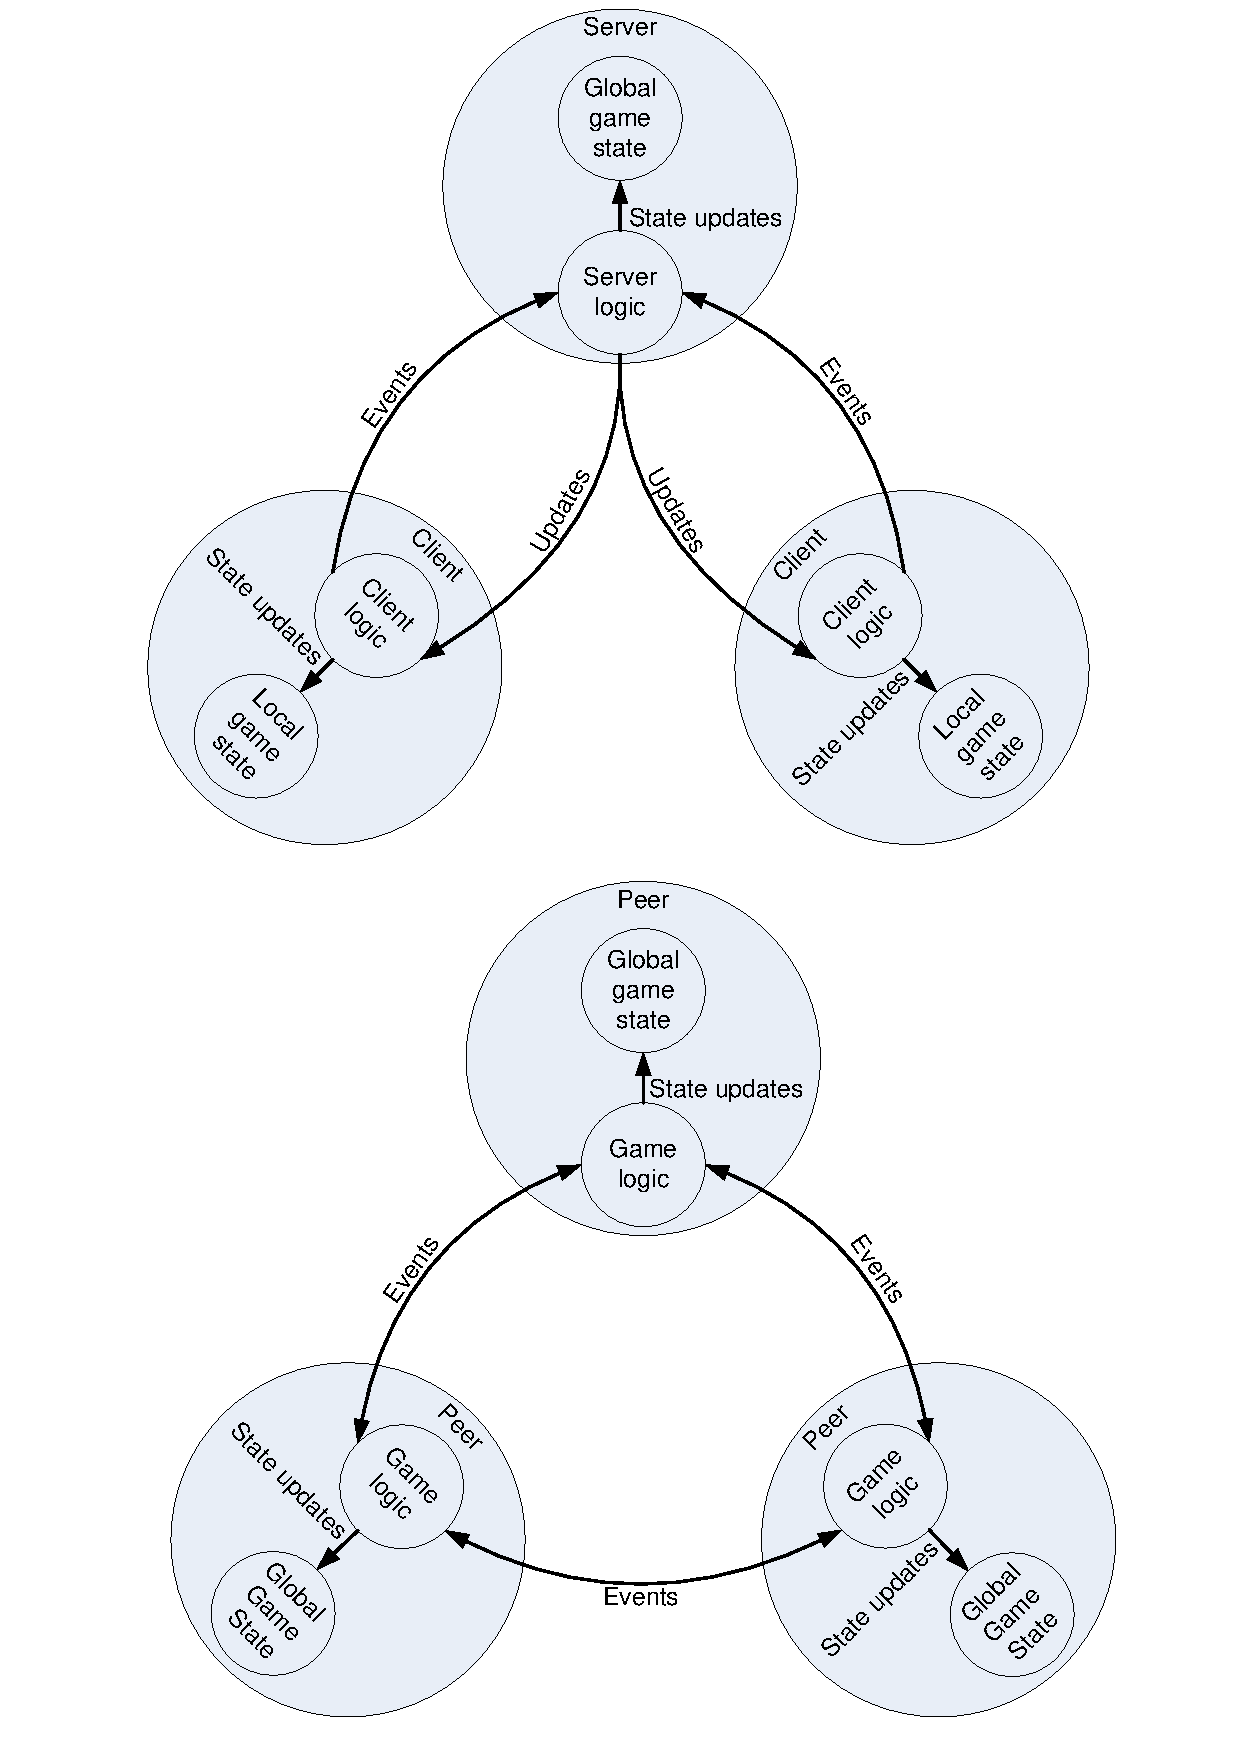
\includegraphics[clip=true, viewport= 2.5cm 15cm 19cm 30cm, width=\columnwidth]{CS_P2P_CMs}}
\caption{Consistency models}
\end{figure}
%
Figure \ref{fig_p2p_cm} shows the fully distributed model. The state persistency model for this consistency model is that the complete game state is
stored on each peer. Any event that a peer generates is sent to all other peers. These events are used as inputs to the game logic, which creates
updates, which are then used to update the global game state at each peer. The event-based model works well for strategy games, and was implemented
in Age of Empires \cite{p2p_cm_aoe} and Starcraft \cite{starcraft_network_model}.

The order in which events are received should be the same for all peers, otherwise the game states of different peers may become inconsistent.
Usually some kind of lockstep technique is used to solve this issue \cite{pessimistic_lock_step}. The issue with lockstep is that it reduces the
latency to twice that of the peer with the highest latency. Various techniques have been proposed that improves the latency by introducing some
deadline before which all events should be submitted \cite{cheat_proof_event_ordering}. This, however, makes it impossible for a player with a high
latency to play the game with anyone other than from her own continent. When latencies issues are not present and all players possess reasonable
latencies, the event-based model can provide for an high-degree of responsiveness, because of no extra latency being added by a server and no extra
server hop required for communications.

The issue with the event-based model is that it is not scalable, since all peers should connect to all other peers and every event is transmitted to
everyone. This means that as $N$, the number of peers in the network increases, the traffic increases with a factor of $N^2$. The security issues of
the P2P network model, on which this consistency model is based, are also present. Slowdown is also experienced by all players if one player's
latency is below par, since the lockstep mechanism has to wait for all events to be received for that round to conclude.

\subsection{Update-based (C/S)}

An alternative to the event-based model is the update-based model, shown in Figure \ref{fig_cs_cm}. This model is based on the C/S network model. The
persistency model here is that an authoritative global game state is housed on the server and a non-authoritative local game state is housed on all
clients for display purposes. No real game logic is housed at the clients, only on the server. All clients send events to the server, which applies
the game logic and sends updates to the clients, while also updating its own game state.

This approach greatly assists with security, as clients cannot influence the state of any other clients and every client's state depends on updates
received from the server. The server state is also termed authoritative, because if there is a conflict, the server state is always the state to
which the system is expected to return. All the security advantages of the C/S model also apply to this consistency model. Another reason why the
update based model is successful is because it is more scalable then the fully distributed model. More hardware can be used to build a more powerful
server, which can handle more clients. Computer clusters and large server are, however, costly to obtain and maintain.

The update-based model is used in many, if not all, MMOGs currently in operation. This includes games like World of Warcraft, Eve Online and Ultima
Online, to name just a few.

\subsection{Client/Multi-Server consistency models}
\label{cms_models}

%Should I add diagrams here?

Apart from the two classic models, there are also models based on the C/MS network model, which are: shard-based, replication-based, object-based and
zone-based \cite{Hu_voronoi_IM}.

\subsubsection{Sharding}

The consistency model that is exemplified by having a state persistency model where the game state (world) is duplicated over multiple servers, with
players connecting to one of these servers is termed ``sharding''. Clients are not able to interact or communicate with players on other shards,
which reduces game immersion. This method does, however, allow for a more scalable system as maximum load is fixed.

Players are not able to enter a shard if that shard has reached its capacity. In the past, this has caused unhappiness amongst players, since popular
shards could be difficult to log in to. Players are also reluctant to move to a new shard, because a lot of time is invested in their characters in
their ``home'' shard. Sharding doesn't allocate resources efficiently, as one shard may be overpopulated while another is underpopulated. For all
practical purposes, this approach is still merely a C/S approach, with players forced into a specific C/S environment.

The benefit of sharding is its ease of implementation and the reduction of content designer load. Because no inter-server communication is required
and no server migration is supported, this method greatly simplifies the server design process. Another benefit of sharding is that it allows for a
relatively small game world to support many players because of the duplication of the worlds. This reduces the load on level designers and content
designers, who now have to populate a much smaller world with content.

\subsubsection{Replication-based}
%Redundant
The replication-based model is similar to sharding, with the difference that all servers share the same duplicated game state. Each server contains
the global game state and clients connect to any one of these servers (mirror-servers \cite{mirrored_server}) or through a load distribution
algorithm to a server (proxy-servers \cite{proxy_server_dist}). Each server handles all actions from clients and updates its own database. The
servers in turn send updates to each other over a high quality link, such as fibre, to maintain database consistency at high speeds.

The problem with this system is that the world is never truly consistent and that there are no optimally chosen inconsistency obfuscation boundaries.
In other words, two players standing next to each other in the virtual world, might be on different servers and, therefore, experience two slightly
different worlds.

\subsubsection{Object-based}
%Object based
The state persistency model of the object-based consistency model equally distributes all in-game objects amongst the servers
\cite{object_based_consistency1}, \cite{object_based_consistency2}, \cite{object_based_consistency3}. For an MMOG, most of these objects are expected
to be player objects. The advantage of this method is that the system load is fixed for a certain player population and that the load is equally
distributed amongst all servers. This allows for more accurate prediction and provisioning of resources, but still does not handle transient loads
well.

Another issue is inter-server communications for this architecture. The inter-server communications are random and also more than the inter-server
communications for a region based system. The reason for this is that the number of player interactions increase with a decrease in the distance
between the players. Players playing together move together, chat and interact with NPCs together. For a region based model, all player-neighbour
interactions remain local to the server.

\subsubsection{Zone/Region-based}
%Zone-based
The state persistency model of the zone-based consistency model divides the virtual world into zones or regions, which are hosted on different
servers \cite{zone_based_stat}, \cite{zone_based_dyn}. A well known example of this model is Eve Online. Busy regions are hosted on their own
servers, while multiple quiet regions are hosted on a single server. This is termed the static region approach \cite{zone_based_stat}.

The issue of the static region approach is that it does not scale well when one region is suddenly populated with players. This type of behaviour
happens quite regularly and is known as flocking \cite{flocking}. When players find something of interest in a region, many players will flock to
that region. The solution to flocking has been over provisioning of resources to handle peak loads, which suffers from the disadvantages discussed
above. Also, if the load changes, the server has to be brought off-line in order to balance the regions.

Dynamic regions are being investigated, where regions can be dynamically shifted from one server to another, in order to balance load
\cite{zone_based_dyn}. This approach adds overhead and significant complexity with regards to the migration of the data and the handling of player
actions while the data are in transit.

\section{Generic state consistency architecture}

\chapter{Peer-to-peer MMVE state management and persistency models}
\label{p2p_mmog_state_persistency}
%%%%%%%%%%%%%%%%%%%%%%%%%%%%%%%%%%%%%%%%%%%%%%%%%%%%%%%%%%%%%%%%%%%%%%%

This section identifies state persistency techniques used in P2P MMOGs. To achieve state persistency in P2P MMOGs, a type of distributed storage is
required. Two classic distributed storage architectures are the Network File System (NFS) \cite{NFS4_protocol} and Coda
\cite{Kistler_Coda_disconnected}. There are, however, some major differences between the requirements of a P2P state persistency model and the
classic distributed file storage model.

Firstly, NFS and Coda still require servers. One of the main advantages of P2P MMOGs is that servers are, for the most part, not required. The other
requirement is low latency file storage and retrieval, which NFS and Coda also do not address. Conflicts are also an issue with the Coda system,
which allows multiple nodes to modify the same object. Despite the many differences, the divergent applications share some of the same requirements,
including: scalability, reliability, security and responsiveness.

The requirement of disconnected operation is generally not applicable to most interactive online games, where a player has to stay connected to the
world, to be able to interact with it. One area where disconnected operation might be of interest to game state persistency is in the area of mobile
gaming. A major challenge for mobile games is the large variances in network latency. Such networks require games that are resistent to network
jitter.

One approach has been proposed in \cite{Chandler_disconnected_games}, where every game client serialises its game state and distributes this game
state to all other clients. Each client then creates some target game state from all received game states as well as its own state. The game client
then attempts to manipulate all NPCs in the game in order to achieve the target game state. The target game state is constantly updated and thus
remains a moving target. This is a new type of consistency model with many research opportunities.

%Overview of four approaches
Four approaches have been identified by which state persistency is achieved in P2P MMOGs: \emph{super peer storage}, \emph{overlay storage},
\emph{distance-based storage} and \emph{hybrid storage}. These four storage architectures are detailed in Sections \ref{super_peer_storage},
\ref{overlay_storage}, \ref{hybrid_storage} and \ref{distance_based_storage}.

%Centralised storage
Two other types of storage sometimes described in P2P MMOGs papers are \emph{centralised storage} and \emph{individual storage}. Centralised storage
is storage in a centralised database, the same as for a C/S MMOG \cite{badumna_engine}, \cite{rooney_centralised_storage},
\cite{hybrid_p2p_cs_centralised}. Centralised storage for an MMOG requires the same large expensive servers and high bandwidth as required by a
classic C/S architecture and therefore does not fit into the P2P MMOG paradigm. For this reason, centralised storage will not be evaluated in this
paper.

%Individual storage
With individual storage, player data are stored on a player's own computer \cite{individual_storage1}, \cite{cheat_proof_playout}. These
architectures do not address the storage of NPC state or mutable objects. These objects cannot be as easily mapped to a single node in the network as
player state can and therefore require a mapping mechanism to decide where to host these objects. Individual storage will not be explicitly discussed
in this survey, however, individual storage can be regarded as a subset of distance-based storage, which will be discussed in detail in Section
\ref{distance_based_storage}.

\begin{table}[htbp]
\centering
\begin{tabular}{|r|c|c|c|c|c|l|}
\hline
Storage type & Reliability & Responsiveness & Security & Fairness & Complexity & Examples\\
\hline
Super Peer & Medium & High & Low & Low & Very Simple & \cite{knutsson_p2p_first}\\
Overlay & High & Low & Medium & High & Simple & \cite{Douglas05enablingmassively}, \cite{using_freenet_storage},
\cite{Fan_phd}, \cite{past_storage_focus}\\
Hybrid & High & High & Medium & Low & Complex & \cite{zoned_federation}, \cite{hybrid_storage1}\\
Distance-based & Medium & High & Low & Medium & Very Complex & \cite{Buyukkaya_voronoi_state_management}, \cite{Hu_voronoi_IM},
\cite{colyseus_distance_based}, \cite{solipsis}\\
\hline
\end{tabular}
\caption{Differences between storage mechanisms} \label{tab_storage}
\end{table}
%
Table \ref{tab_storage} presents a characterisation of current storage systems according to the characteristics defined in Section
\ref{key_challenges_cm}. Table \ref{tab_storage} also provides some references that act as examples of the different storage types mentioned. These
example architectures will be discussed in detail in the sections to follow. The purpose of the complexity category in Table \ref{tab_storage} is to
provide a measure of how difficult it will be for an application developer to use any of the storage types and is discussed in Section
\ref{recommendations}.

\section{Characteristics}
\label{key_challenges_cm}

%Consistency issues
The key challenges related to P2P MMOG persistency models identified during this literature study were: scalability, reliability, responsiveness,
security and fairness. All state persistency models will be reviewed with these characteristics in mind. In order to evaluate any persistency model,
metrics have to be defined to measure the key characteristics of a storage system. This will allow for different persistency models to be compared
and provide a measure of the applicability of any persistency model to P2P MMOGs.

\subsection{Scalability}
Scalability underpins all evaluation criteria. This implies that for a system to be scalable, all other evaluation criteria should be satisfied for
large numbers of nodes and data. For this reason, scalability will not be explicitly reviewed in the following storage types. Rather, all other
evaluation criteria will be evaluated for a large number of nodes, thereby taking into account scalability.

The question of what constitutes a large number of nodes arises. To establish what an adequate number of nodes is, current MMOG architectures can be
used for inspiration. It is proposed that to classify a system as \emph{sufficiently scalable}, the smallest number of peers that should be used is
approximately 3000. This is the number of players per server, currently supported by most active C/S MMOGs. For a system to be classified as
\emph{truly scalable}, it is believed that the architecture should support 60,000 concurrent users, twenty times more than a sufficiently scalable
system. This is the number of peak concurrent users (PCUs) currently supported by the super computer used to host Eve Online \cite{eve_pcu}. These
two measures will ensure that a system is as scalable as other currently available architectures.

For systems that will support the MMOGs of the future, it is believed that a target of 1 million nodes should be used. This number is sixteen times
that of a truly scalable system and the peak concurrent player count of World of Warcraft in China in 2008 \cite{WoW_china_pcu}. Systems that will
support these numbers can be classified as \emph{highly scalable}. It is important to note that no current systems support such a large PCU count on
a single server cluster. The PCU count presented for WoW is the PCU count over all server clusters hosting WoW in China.

\subsection{Fairness}
Ensuring fairness in the system means distributing load evenly according to the abilities of individual nodes. This ensures that not only a small
number of nodes provide all system resources required for the system to function, but that all nodes contribute what they can, in order to support
the system.

Fairness can be evaluated by evaluating the distribution of game state amongst all nodes in the P2P network. This can be measured at a file level,
i.e. what is the variance of the number of files contained on each node, or on byte level, i.e. what is the variance of the number of bytes stored on
each node. A lower variance will point to a fairer data persistency scheme.

\subsection{Reliability}

For the storage to be reliable, it must be impossible for data to be lost, and stored data should always be available when a node requests it.
Reliability encompasses both robustness and availability. Robustness means that the data should be resilient to network churn and availability means
that data should be available to any node in the network, with the correct permissions.

\subsection{Responsiveness}

To ensure system responsiveness, data must be stored or retrieved in real-time. With real-time, it is meant that data should be available within a
certain time frame that would ensure correct functionality of the MMOG requiring it. The variance in data retrieval times should be small.
Responsiveness can be measured by the time it takes for an object to be available for reading, anywhere in the network, after having been written.
How long it takes to read or write data to the storage network can also be measured.

\subsection{Security}
\label{characteristics_security}

The storing system should store data securely. It should not be possible for data to be altered in ways that are inconsistent with the game rules. It
should also be possible to identify nodes that alter the data in a malicious way. This also adds the requirement that nodes should be authenticated
in the storage system and that only authorised nodes should be able to alter data. Security is the combination of a number of objectives:
Authentication, Authorisation, Data Integrity, Confidentiality, Availability, Trust, Privacy and Identity Management
\cite{distributed_systems_security}.

For a state persistency model to address the security objectives of authentication, authorisation, confidentiality, trust, privacy and identity
management, a certification scheme with public and private key encryption is required. Such a scheme allows for the identification of users, and by
having users sign any storage interactions, every change made to the storage system can be tracked. This is a major differentiating factor from
classic distributed storage systems such as Freenet, where a primary objective is anonymity. If all operations are logged and all users have to be
identifiable for a secure system, no users can truly be anonymous.

\section{Super peer storage}
\label{super_peer_storage}

%Super peer storage - description
Super peer storage relies on the super peer storing all information that is in its domain. A domain is usually created by segmenting the world into
regions and super peers act as regional servers to all peers in their region. Each super peer handles all game logic and distributes updates to all peers in its region. The super peer also handles state persistency for its region, hosting NPCs, objects and persistent player data.

\begin{figure}[htbp]
 \centering
 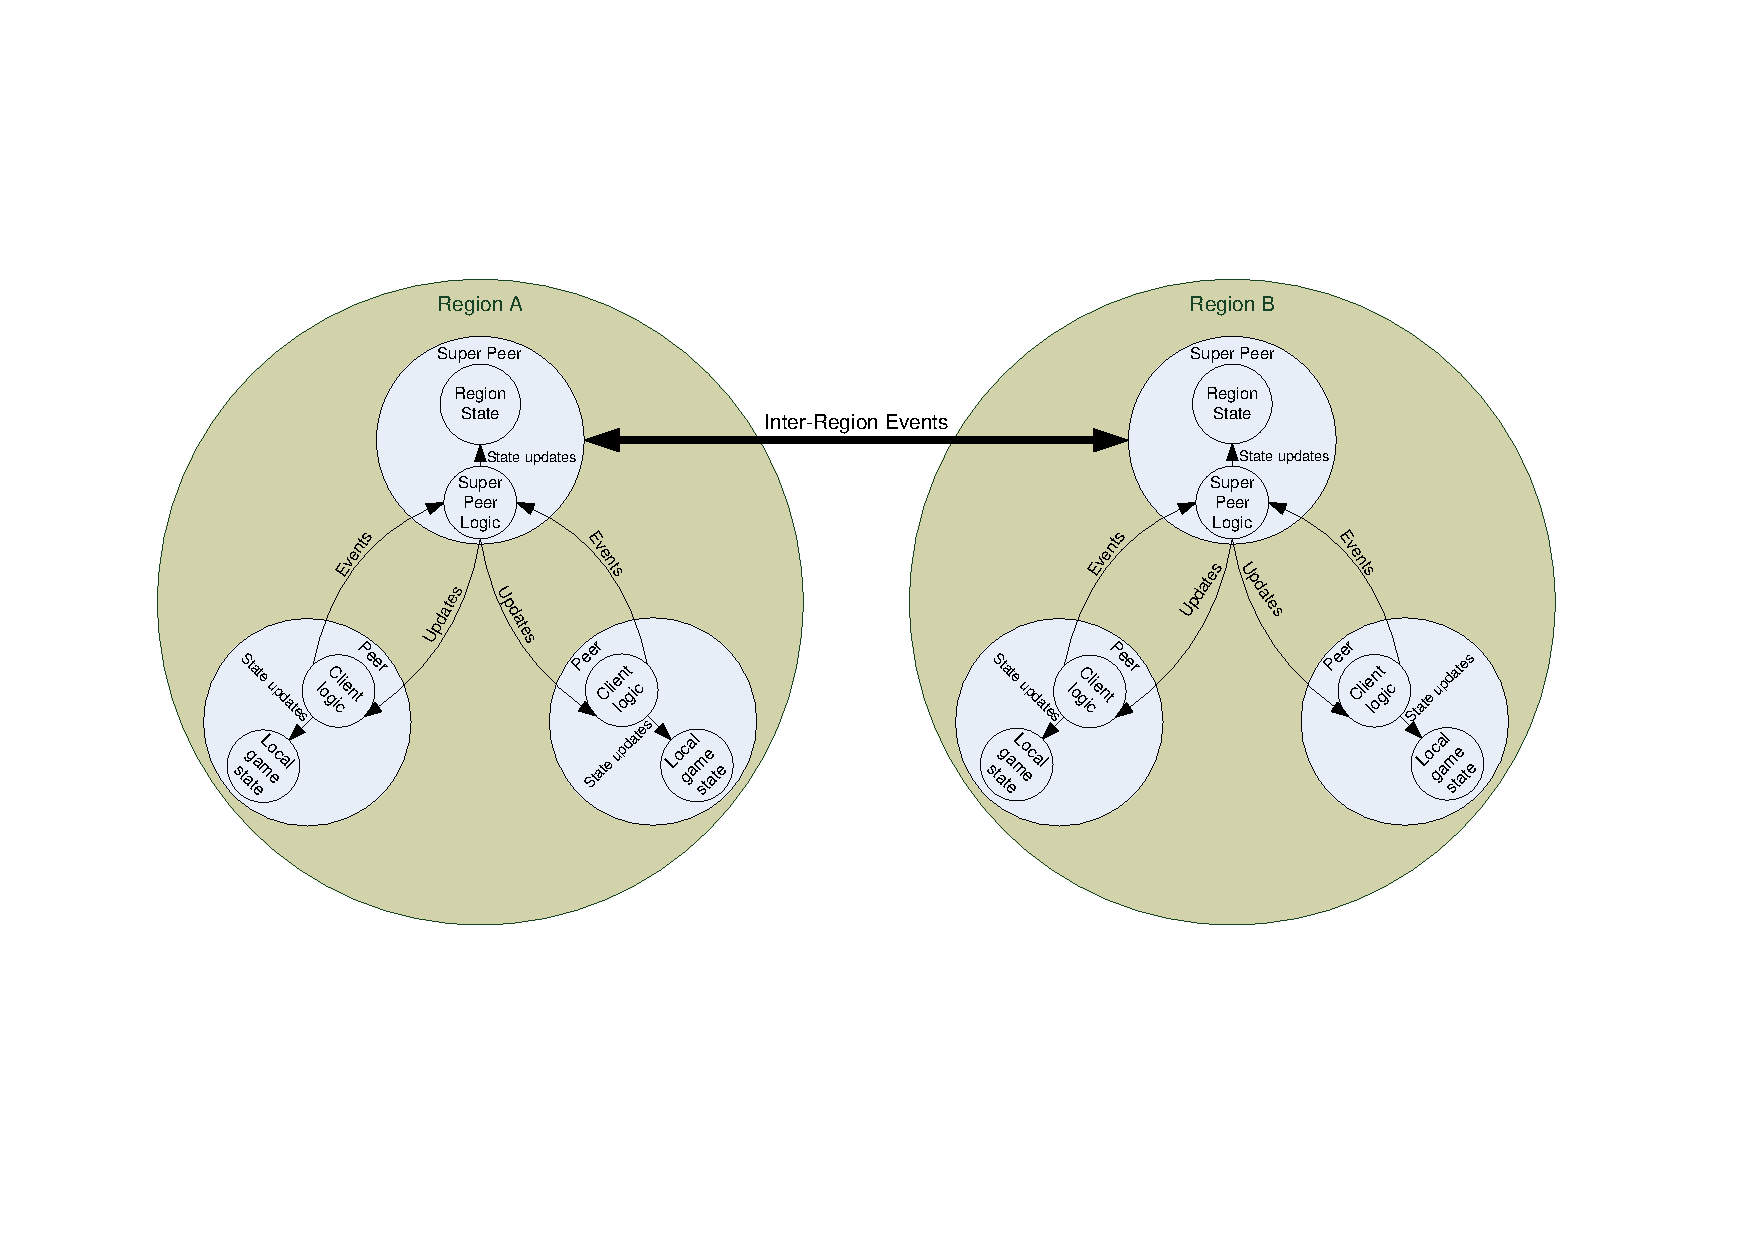
\includegraphics[clip=true, viewport=2cm 5cm 27cm 16.5cm, width=\textwidth]{region_based_CS_CM}
 \caption{Region-based Client/Server consistency model}
 \label{fig_cs_region_cm}
\end{figure}
%
The consistency model for this approach is depicted in Figure \ref{fig_cs_region_cm}. One can see that this approach is modelled on the update based
model, but segmented into separate regions. The role of the server is here fulfilled by a super peer, which is a peer that is selected in some
logical way, from the available set of peers and then promoted. Server selection in itself is a complex topic that has to deal with determining
whether a peer has sufficient resources available and also whether the peer is trustworthy.

Each super peer in this model houses the complete region state as shown. Super peers also house the game logic. Clients in the region only house
copies of the regional objects and some client logic to update the local copies of objects. Like the C/S model, clients only send events to super
peers, where super peers apply the game logic and send state updates to clients.

\subsection{Fairness}
%Super peer storage - issues
The super peer storage model has many potential issues. Overloading of the super peer is one. A super peer could be relatively easily overloaded if a
region becomes too crowded, since a super peer is merely the computer of some player in the game and not a specialised server machine. The question
of fairness also arises. The idea of a P2P MMOG model is that all peers share resources. With this model, peers with extra resources are expected to
donate these resources for the good of all. Players might consider it unfair, when they are constantly expected to donate resources, some of which
they might have to pay for, while other players never contribute.

In a system with lower fairness, the individual user load is also higher for those users that do have to contribute resources. This means that in an
unfair system, the users that do have to contribute, have to contribute more than what they would have, were it a fair system.

\subsection{Reliability}
\label{super_peer_storage_reliability}

In a P2P system, with a high rate of churn, players are expected to constantly leave and join the network. Because of this reality, redundancy
mechanisms have to be developed that would ensure state data are always available, even when a super peer leaves the network. It is possible to solve
these issues by having redundant super peers in each region that take over hosting responsibility when the main super peer leaves.

It is important that the main and backup super peers always possess consistent states, even during a transition from main to backup. Other schemes to
support improved reliability deal with reputation mechanisms for super peers. Super peers that have more resources and stay in the network longer are
preferred during super peer selection, using reputation mechanisms \cite{fan_mediator_paper}.

\subsection{Security}

Probably the most important issue is that of security. If a single peer is allowed to house the player information of a large group of players, it
might become possible for such a peer to maliciously modify the data. The issue is not only that modification of the data might be possible, but also
that it would be impossible for the cheating to be detected, because of no centralised logging. Locally obtaining access to data will circumvent the
protections created by a certification system, which would then pose a threat to all security objectives protected by the certification system as
mentioned in Section \ref{characteristics_security}.

A scheme that would improve the reliability of this systems has been proposed, where every event is also sent to the backup super peer of the region
\cite{past_storage_focus}. The main super peer responds with the update and the backup super peer responds with a hash of the update. A peer can then
check whether the hashes match to determine whether the data has been received correctly. A hash is not the state update itself, so will be smaller,
but the events that have to be sent to all super peers will increase traffic in the network and bandwidth usage by peers.

\subsection{Responsiveness}
There are also advantages to super peer storage. All data are stored on the super peer, which means that storing data is a low latency operation. The
regional state can be stored and retrieved at high speeds, making the system very responsive. Data retrieval from such a storage is as fast as data
retrieval from a server. Peers can request data from a super peer and the data can be returned to the peer in one hop after transmission of the
request. Super peers may, however, become overloaded with requests and thereby increase the latency of the system.

\subsection{Existing architectures}

Knuttson et al. \cite{knutsson_p2p_first} employ regional super peers called ``coordinators'', to host all shared object states. The coordinator is
chosen as the node whose ID is closest to that of the region ID. The region ID is a SHA-1 hash of the region's textual name \cite{SHA}. This mapping
makes it unlikely that the coordinator will be a member of the region. The advantages of such a selection scheme is that the opportunities for
cheating are reduced, because the data are hosted on a peer that has no or little interest in the data, as described in Section
\ref{distance_based_storage_security}.

Coordinator hand-offs also occur less than if the coordinator was an elected member of the region. If this is the case, a new coordinator has to be
chosen every time the current coordinator leaves the region. In this scheme, hand-offs only occur as a result of network churn, which is far lower
than the number of players moving from one region to another.

Reliability is achieved by maintaining backup coordinators as the Distributed Hash Table (DHT) neighbours of each region coordinator. One method by
which redundant region coordinators are maintained in \cite{knutsson_p2p_first}, is to create backup coordinators on peers with IDs closest to the
current coordinator. This means that if the main coordinator fails, all data will automatically be routed to the backup, because of the feature of
DHTs. This method is similar to how reliability is achieved in overlay storage as described in Section \ref{overlay_storage_reliability}.

\section{Overlay storage}
\label{overlay_storage}

Overlay storage is classified as using any type of structured P2P overlay to store data in a distributed fashion. This is a very broad definition,
which basically encompasses any P2P distributed storage currently in use. Some examples and a comparison of different distributed storage techniques
can be found in \cite{Hasan_distributed_storage_survey}. The reasoning is that any P2P distributed storage can be used to only store game files.
Therefore, distributed storage is used as a distributed database for game files. Whether this is an optimal solution will be discussed in the
remainder of the section.

\subsection{Reliability}
\label{overlay_storage_reliability}

Overlay storage can be made reliable, using redundancy. One method used to achieve high reliability in structured overlay storage is to store $k$
replicas for any file stored, in order to ensure the availability of the file. These replicas are stored at the neighbouring nodes of the node
containing the original file. Neighbours are the $k$ nodes whose IDs are closest to that of the root node. By the characteristics of DHT
distance-based routing, if the node with the original data leaves the network, packets will automatically be routed to the neighbouring node, which
stores a duplicate. This technique ensures high availability of data and the number of duplicates can be chosen according to the reliability of the
network.


\subsection{Responsiveness}
%Overlay storage - issues

The most significant issue with overlay storage is the delay incurred when storing and retrieving data. As data can be stored anywhere on the network
and the network is not fully connected, an average of $\OO{\log(N)}$ hops are required to retrieve or store a data item
\cite{storage_and_chaching_PAST}. Although this is a sufficient order complexity for a routing algorithm in a large network, it is not sufficient to
support a real-time application. For responsive MMOGs, a distributed file system is required that allows for real-time file storage and retrieval.

The mechanism by which churn is handled, described in Section \ref{overlay_storage_reliability}, also improves responsiveness.  This is achieved,
because IDs created by the random hash function ensures that a nodes's neighbours are distributed randomly throughout the P2P overlay. This random
distribution ensures that file replicas, stored at a node's neighbours, are uniformly distributed throughout the P2P overlay network.

%Data migration in Oceanstore

\subsection{Security}
The overlay storage model is more secure than the super peer storage model as data are distributed amongst all peers and redundancy and quorum
techniques can be implemented to ensure that files are retrieved with a high level of security.

To ensure a secure system, copies of files have to be saved at different locations. If a file is retrieved, all copies must be queried and received.
All received copies then have to be compared to ensure that the contents are correct. This introduces additional network overhead as well as
additional load on nodes to serve as file copies.

The network overhead can, however, be reduced by having file replica nodes only send hashes of the files, which may then be compared at the
requesting node. Hashes require less bandwidth, while still allowing a requesting node to check update validity by hashing the received update and
comparing with the received hashes.

\subsection{Fairness}

Overlay storage is fair, as all nodes share file data and requests equally. The system might be made fairer by taking into account the heterogeneity
of peers. Peers do not all possess the same resources, something which a truly fair system should take into account. The difficulty with using such a
scheme is that peers can be made to report incorrect resource information in order to reduce their resource donation requirement. This is where
incentive mechanisms have to be investigated as well as ways to ensure correct resource reporting.

\subsection{Existing architectures}

%Merabi, 2004 \cite{using_freenet_storage}
In 2004, Merabti and El Rhalibi mention the issue of ``Data Storage'' \cite{using_freenet_storage}. It is recognised that a distributed storage
scheme is required and that such a scheme ``\ldots requires careful designing\ldots''. They propose the use of a data storage architecture based on
the Freenet project \cite{clarke_freenet}. Freenet is a distributed storage facility that uses a Darknet to ensure user anonymity when distributing
files. A system such as Freenet is designed for general file sharing, which means that no focus is placed on achieving the high levels of
responsiveness required for MMOGs. While the need for state persistency is briefly mentioned in the 2004 paper by Marabti and El Rhalibi, Douglas et
al. implement a workable solution for state persistency in 2005.

%Douglas, 2005 \cite{Douglas05enablingmassively}
Douglas et al. designed a P2P MMOG architecture in 2005 \cite{Douglas05enablingmassively} and implemented state persistency using a distributed
storage implementation, which they developed in 2003 \cite{Harwood03hashingspatial}. The storage system allows for the manipulation of spatial data,
while also implementing range queries. This enables the system to store and retrieve data that exist in a certain area of the game world. In the MMOG
architecture they developed, state persistency is implemented by the ``Spatial Data Service'' (SDS), which is a distributed storage architecture that
uses the Chord P2P overlay for routing \cite{chord}.

%Hampel, 2006 \cite{past_storage_focus}
PAST has become a popular way to implement state persistency. This is the approach proposed by both Hampel et al. in 2006 \cite{past_storage_focus}
as well as Fan in 2009 \cite{Fan_phd}. In these publications, it is said that PAST is used to store the global game state, but never is detailed what
is stored and how regularly it is stored. Player information is supposed to be stored as game state, but from the papers it is unclear how position
updates are handled. It is not clear whether the last position of a player is stored at all or how regularly it is stored. It is important to know
how position updates are handled in the game, since position updates are the most common type of update \cite{knutsson_p2p_first}.

PAST has not gained much commercial adoption, because of the lack of support for keyword searches, which is a requirement of most distributed storage
networks, where users constantly search for content. Keyword searches are, however, not required by the storage mechanism of an MMOG. The IDs of the
items stored in the network will be known. A player's inventory can, for example, always be called \verb.(player_name)_inventory.. A hash of this
file name will find the correct file. This, and the use of Scribe, is why PAST has become popular with researchers of P2P MMOGs.

PAST \cite{PAST_storage} uses Pastry to implement a distributed storage system. Files that have to be stored are given IDs, by using some hash
function, for example SHA-1 \cite{SHA}. The file, along with the ID are sent as a message over the overlay. The messages is then routed to the node
whose ID is a closest match of the file ID, where the file is stored. If any nodes wish to retrieve the file again, it only requires the file hash. A
``get'' message can be sent to the overlay, where the overlay will route the message to where the file is situated and retrieve the file.

In an effort to increase responsiveness, PAST also employs caching techniques \cite{storage_and_chaching_PAST}. If a node forwards many queries for a
file, that node can elect to cache the file to improve the responsiveness of the system. This caching can only occur if the node has space available.
If a node has cached a file and another file is explicitly inserted into the node, it can elect to remove the cached file in order to free up space.
This means that the success of the caching mechanism is directly related to the level of storage utilisation. Higher utilisation will prevent files
from being cached.

The main difference between the implementation by Douglas et al. and the PAST implementations, is that the former supports range queries on spatial
data, which allows for a set of objects to be returned, queried by their virtual in-game position. With PAST, the exact ID of an object is required
before it may be retrieved. Using PAST is the simplest means by which game state persistency may be implemented, but PAST is not necessarily the
application best suited to game state persistency. There exists a need for more research into appropriate state persistency mechanisms for P2P MMOGs.

\section{Hybrid region-based storage}
\label{hybrid_storage}

%Overlay storage - description
\begin{figure}[htbp]
 \centering
 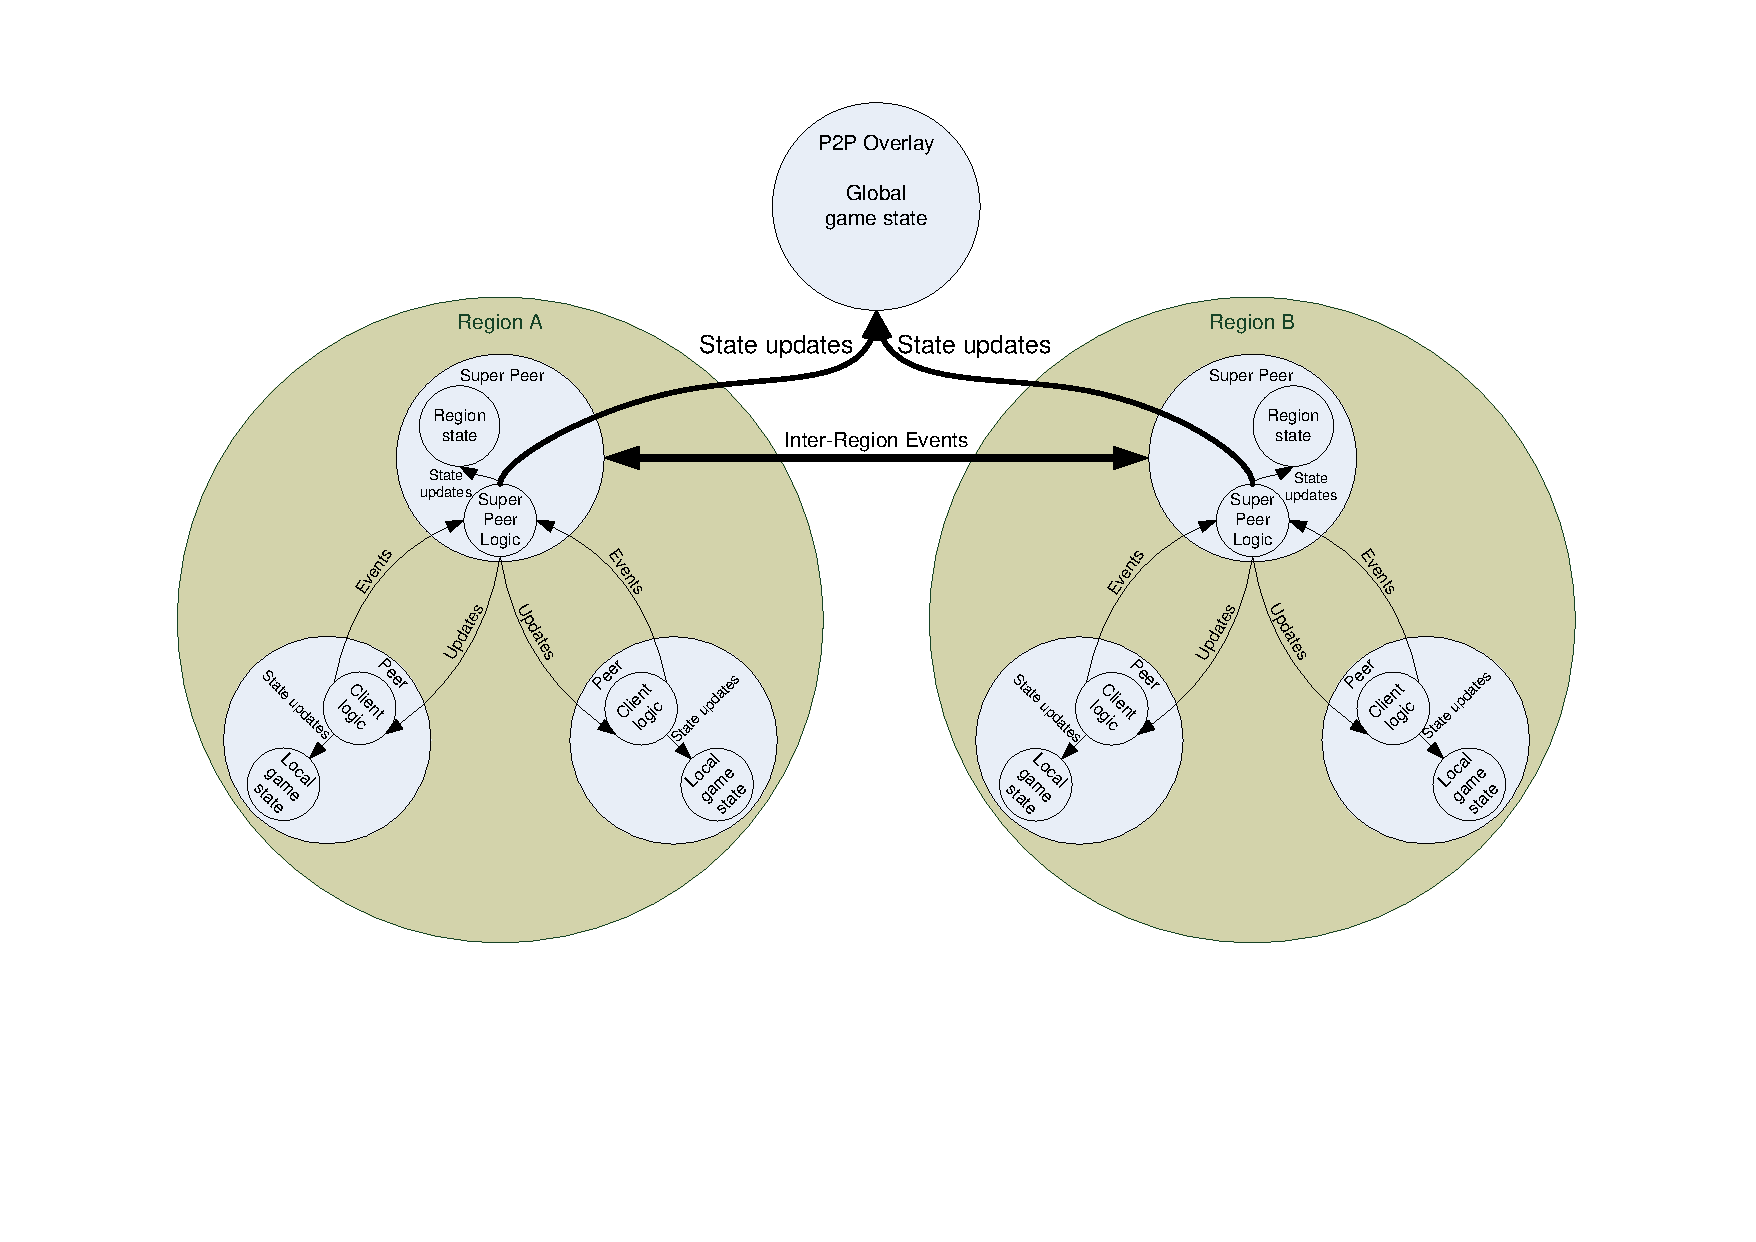
\includegraphics[clip=true, viewport=2cm 5cm 27cm 19.5cm, width=\textwidth]{region_based_CS_CM_P2PO}
 \caption{Hybrid region-based super peer storage with backup overlay storage consistency model}
 \label{fig_cs_region_o_cm}
\end{figure}
%
Figure \ref{fig_cs_region_o_cm} shows a type of Super Peer/Overlay hybrid storage implemented in \cite{zoned_federation}. The model depicted in
Figure \ref{fig_cs_region_o_cm} uses an overlay storage, managed by regional super peers. The world is divided into regions, with each region
controlled by a super peer. The complete region state is cached at every super peer, the same as with super peer storage. There also exists a backup
overlay storage architecture, to which data may be backed up for long term, redundant and secure storage. The hybrid region-based overlay storage
contains many improvements over pure overlay storage as will be discussed in the following sections.

\subsection{Reliability}
\label{hybrid_storage_reliability}

Because of the use of overlay storage for backup, the hybrid region-based storage is almost as reliable as a pure overlay storage. It is classified
as almost as reliable, because there is a delay between when data changes and when it is updated in the overlay. If a super peer fails during this
time and the data was not backed-up to the overlay, that data could be lost. Backup super peers can, however, be implemented as described in Section
\ref{super_peer_storage_reliability} to improve the reliability of the hybrid storage model.

\subsection{Responsiveness}

Because all regional files are cached at super peers, the system is as responsive as super peer storage.

\subsection{Security}

Security in hybrid storage is still an issue, because of the inherent problems of the super peer storage model. Although it is more difficult for
nodes to access and manipulate data stored in the overlay, a malicious node promoted to super peer status may manipulate the region data it controls.

It does seem possible to achieve higher levels of security, by checking data received from super peers, against the data stored in the overlay. Care
should be taken with such a scheme, because the rate of change of data at the super peers might be higher than the rate that data are submitted to
the overlay. Another issue is the time delay between data received from a super peer and data received from the overlay.

\subsection{Fairness}

The issue of unfairness is also still present in hybrid storage. The system is fairer in that all nodes share the load of the overlay storage, but
there still exists the unfairness of the super peer storage. As all data exists in both the overlay storage as well as the super peer storage, the
system is as unfair as super peer storage, because the same quantity of data as in super peer storage is not being distributed evenly amongst all
nodes.

\subsection{Existing architectures}

\begin{figure}[htbp]
 \centering
 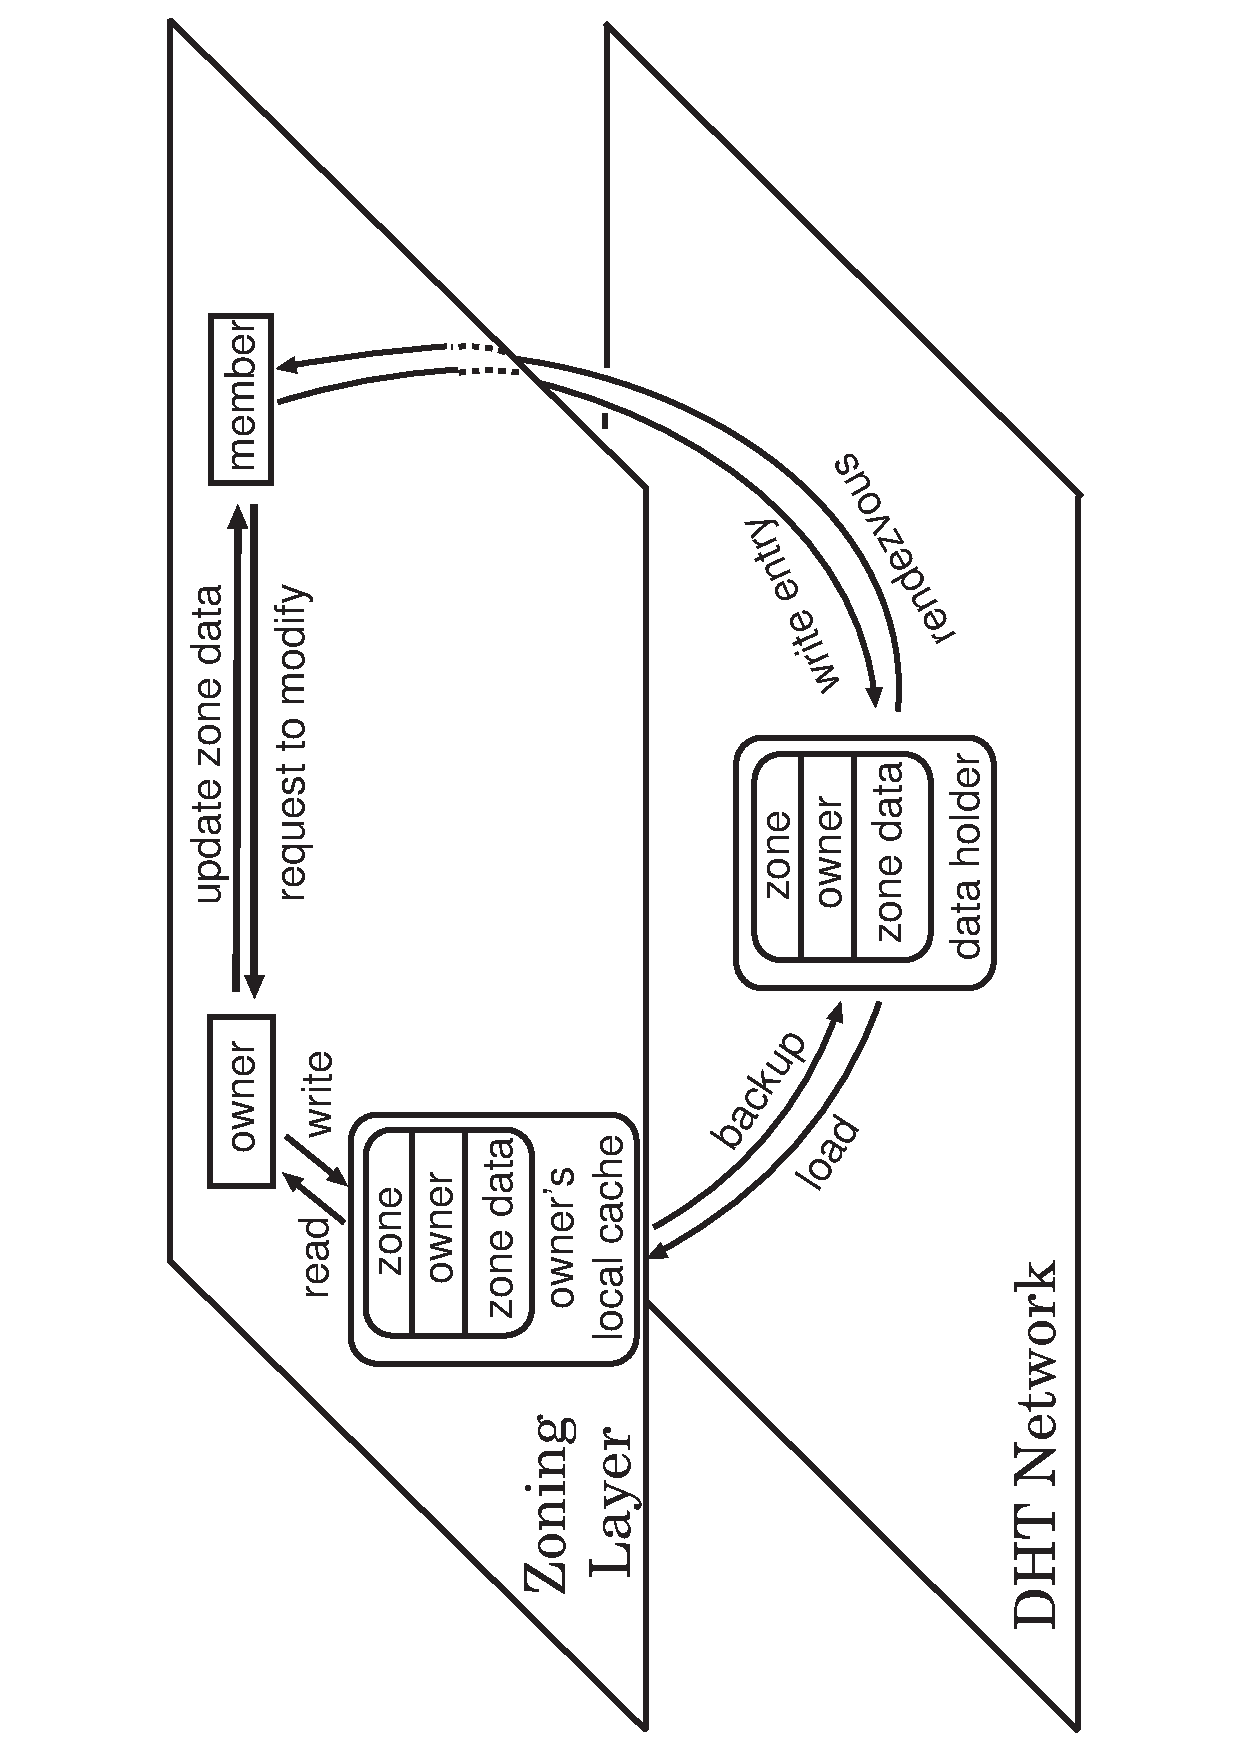
\includegraphics[clip=true, viewport=2cm 0cm 19cm 30cm, angle=-90, width=0.5\columnwidth]{zoned_federation_model}
 \caption{Zoned Federation Model \cite{zoned_federation}}
 \label{fig_zoned_federation_model}
\end{figure}
%
The first hybrid state persistency model for P2P MMOGs was proposed by Iimura et al. in 2004 \cite{zoned_federation} and called the ``Zoned
Federation Model'', shown in Figure \ref{fig_zoned_federation_model}. The regional super peers are called ``Zone Owners'', which handle all events by
clients in their zone or region. In the Zoned Federation model, a Zone Owner acts as the primary storage medium for all object states in the zone or
region. As shown in Figure \ref{fig_cs_region_o_cm}, this is analogous to an update based model, divided into zones. The difference here is that the
game state of all zone owners are regularly backed-up to overlay storage. The zoned federation model can thus be seen as a super peer/overlay storage
hybrid. The super peers storage provides for low latency data storage and the overlay storage provides security and reliability.

An extended abstract, published by GauthierDickey et al. in 2004 \cite{hybrid_storage1}, proposed to distinguish between permanent and ephemeral
data. Permanent data are described as data that should exist at all times and ephemeral data are described as data that need only exist for as long
as its owner is in the game. An item, being dropped by a dispatched NPC, can be considered as ephemeral. When the peer on which the data is hosted
leaves the area, that item can disappear. An example of permanent data is a player's inventory contents, which can further be classified as
participatory data or a player's house, which can be classified as existential data. Participatory data are data that need only be available when a
specific player is in the game and existential data are data that should be available, even when a certain player is not present in the game.

Categorising data by how long and under which circumstances the data should exist, may assist in the design of the storage model. Since ephemeral
data does not have to exist after the player has left the game, it may be stored in primary memory. Participatory data might also be stored on the
player's computer, but security issues will have to be kept in mind. Existential data will have to be stored somewhere other than on the player's
computer, since other players will require the data, even in the absence of the player that might have left the game. GauthierDickey et al. did not
explore how their data classification scheme might be translated into a state persistency model.

\section{Distance-based storage}
\label{distance_based_storage}

%Distance-based - overview
Distance based approaches, such as the Voronoi storage approaches \cite{Buyukkaya_voronoi_state_management}, \cite{Hu_voronoi_IM} and some more
general approaches \cite{colyseus_distance_based}, \cite{solipsis}, store object data on the peer closest to the object in the virtual world. Some
distance metric is used to determine on which node an object should be stored.

\begin{figure}[htbp]
 \centering
 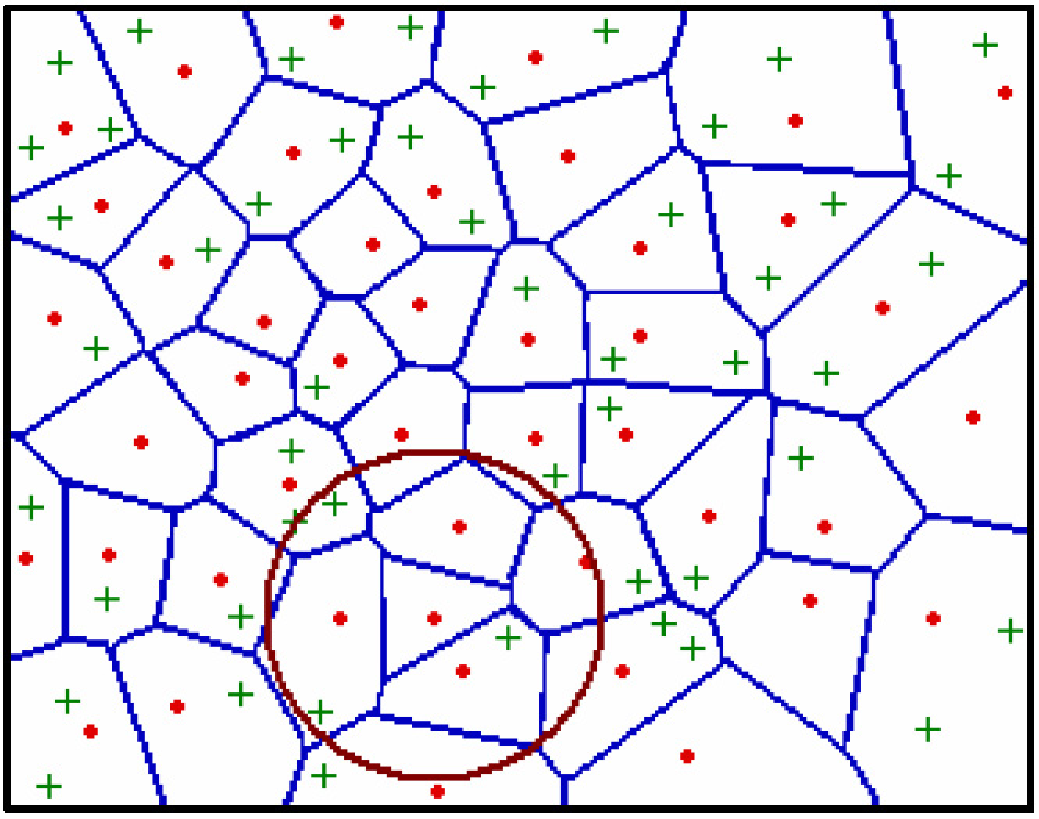
\includegraphics[width=0.4\columnwidth]{voronoi_diagram}
 \caption{Voronoi Diagram \cite{Buyukkaya_voronoi_state_management}}
 \label{fig_voronoi_diagram}
\end{figure}
%
Given a set of points, the Voronoi diagram of the set of points is the partition of the plane, which associates a region around every point in such a
way that all other points contained in the region are closer to the centre point than any other point in the set. Figure \ref{fig_voronoi_diagram}
shows a Voronoi diagram, where the lines define the region boundaries, the dots define the players, which make up the set of points for which the
diagram was calculated, the plus signs represent mutable objects and the circle represents the AoI of a central point in the set.

For the Voronoi approaches, described in more detail in Section \ref{distance_based_existing_archs}, a node controls and hosts all objects within its
Voronoi region. The reasoning is that there is a high probability that the player closest to the object is also the player using the object. Examples
of this are where a player is trading or fighting with an NPC.

\subsection{Responsiveness}

%Distance-based - issues
An issue with the above reasoning is that multiple nodes are usually interacting with a single object. The examples of the NPC monster and trader are
again relevant. Usually many players interact with a trader NPC and usually players attack monster NPCs in groups.

Multiple player interactions are, however, not as big an issue as others have suggested \cite{Fan_deisgn_issues_p2p}. In the best case, the object
being used by a player is also hosted on that player's node. If another player requires use of a remotely hosted object, that player may still
interact with the object, where the host node is now acting as a server to that player. This means that every player hosting an object becomes a
server for that object. In the case where a player interacts with an object hosted locally, there is no object latency. In the case where a player
accesses a remotely hosted object, there is only one hop latency, the same as with a C/S or super peer application.

Issues with this approach stem from the fact the players are constantly moving. When players move, the objects in their regions change. Objects,
therefore, have to be constantly handed over from one peer to another, which might cause significant network traffic. An object in transit might also
delay interaction with that object. Because object transfer introduces overhead into the system, how regularly an object has to be transferred and
whether the number of transferrals produce sufficiently low overhead to implement a real-time game, still have to be investigated.

Voronoi-based storage schemes also become unresponsive when communications are no longer between neighbours, but between two arbitrary nodes in the
Voronoi overlay. When such communications occur, the average required time to route a message is $\OO{N^{1/2}}$ for a two-dimensional configuration.
Advancements have been made that suggest augmenting the Voronoi overlay with additional links to far off nodes to create a small world network. This
reduces the average routing time to $\OO{\log{(N)}}$, the same as for overlay storage \cite{Steiner_voronoi_shortcuts}.

\subsection{Reliability}

Reliability, because of network churn, is still an issue. Nodes will leave the network whenever a player stops playing the game, which makes it a
common occurrence. When nodes leave the network, the objects that are stored on that node should still be accessible to other players. This will
require transferring all objects contained in the leaving node to another object, still present in the network. No papers have yet dealt with the
issue of reliability in a distance-based storage network.

The same solution that is used for overlay storage, namely the presence of redundant peers, might also be implemented for distance storage. Another
structured overlay might be used to implement this redundancy in exactly the same way it is done with hybrid storage mentioned in Section
\ref{hybrid_storage_reliability}.

\subsection{Security}
\label{distance_based_storage_security}

The main issue with the distance based scheme is security. Nodes that have the most interest in an object also have the most interest to manipulate
that object in ways inconsistent with the game rules. When objects are hosted on nodes that have the most interest in them, there will be a strong
drive to try and manipulate these objects. Because these modification are all local, it is also not possible to log the alterations and detect
cheating. Means by which local objects can be secured have to be found or distance based algorithms with quorum need to be investigated.

This security issue is similar to that of super peer storage, in that local data can be accessed, thus circumventing the certification system. With
this circumvention, the objectives of authentication, authorisation, confidentiality, trust, privacy and identity management are all compromised.

\subsection{Fairness}

Distance-based storage is relatively fair as all objects are distributed amongst all nodes. Where the system becomes somewhat unfair is when a node
is nearest to a large number of objects. For Voronoi regioning approaches, this is when a peer's Voronoi region contains many more objects than the
average number of objects hosted by other peers. This might not be a major issue, depending on how long the objects have to be hosted on the
overloaded peer. This will depend on the movement of the overloaded peer as well as that of neighbouring peers. The use of aggregators as a proposed
solution to this problem is discussed in Section \ref{distance_based_existing_archs}.

\subsection{Existing architectures}
\label{distance_based_existing_archs}

%Colyseus, 2006
Bharambe et al. created the Colyseus architecture in 2006 \cite{colyseus_distance_based}. The architecture is designed to support First Person
Shooter (FPS) games and implemented to function with Quake II. Mutable game objects are stored on the peer that is nearest to the object in the game
world. An ``object placer'' component is mentioned, but the details of the placement algorithm are left for future work. The architecture also does
not implement non-volatile state persistency, since this is not required for normal FPS games, where object states need only exist to the end of a
round and where players generally do not leave before the end of the round. This means that object states are only stored in primary memory, until
the end of a game round.

%Solipsis, 2008
The Solipsis architecture was created by Frey et al. in 2008 \cite{solipsis}. The architecture uses Voronoi diagrams to create virtual regions.
Stationary objects are maintained by site nodes until a player picks up an object. When an object is picked up, control of that object is transferred
to the player that picked up the object. The Solipsis architecture focusses on distributed physics computation and when a player gains control of an
object, that player is responsible for the object's physics computations. That player should also save all object state until a new player takes the
object, at which time control is transferred to her. Control can also be transferred back to a site node if an object remains stationary for some
time.

What differentiates the Solipsis distance-based storage from the other architectures presented in this section, is that object states are only
handled by peers as long as those peers directly use an object. At other times, those objects are handled by site nodes. This differs from other
distance-based storage techniques, where all objects that are nearest to a player in the virtual world are controlled by that player.

%Buyukkaya and Abdallah, 2008 and Hu et al., 2008
In 2008, papers were published by Buyukkaya and Abdallah \cite{Buyukkaya_voronoi_state_management}, and Hu et al. \cite{Hu_voronoi_IM}, proposing to
use Voronoi diagrams \cite{voronoi_diagrams_survey} to implement distance-based storage. Voronoi state management schemes host the mutable objects on
the peer in which region the object exists. As peers move around in the virtual world, the Voronoi diagram has to be constantly recalculated and
objects have to be moved to new owner peers as the regions in which they fall change. The significant advantage of the Voronoi approach is that peers
only require connections with their neighbours, and peers within their AoI.

A thesis by Chang also describes the Voronoi approach in more detail and how to achieve game state consistency amongst all nodes in a Voronoi network
\cite{Chang_Voronoi_state_management_masters}. What distinguishes this work from the others is the implementation of a load balancing mechanism. When
peers get overloaded, another, more powerful peer is chosen as an Aggregator. The Aggregator assumes responsibility for a larger area that
encompasses multiple peers. This scheme will reduce the load on peers with minimal resources, but it is uncertain how this would reduce load when
peers with an average number of resources in an area become overloaded.

The works by Buyukkaya and Abdallah, Hu et al., and Chang form part of the VAST project, which is being created to be a fully functional P2P overlay
architecture, using Voronoi diagrams as its basis \cite{VAST}. The reason why state persistency in Voronoi-based P2P MMOGs architectures are mostly
distance-based approaches, is because the Voronoi diagram immediately identifies which objects are closest to a particular peer, and therefore, which
objects that peer has to host. Architectures not making use of Voronoi diagrams still require some other mechanism to identify which objects which
peers should host.

\section{Summary and recommendations}
\label{recommendations}

Supper peer storage can be seen as a C/S type storage implementation, where every region has a super peer that stores all data for that region.
Overlay storage is a fully distributed, P2P approach to storage, where every node stores data as part of a P2P overlay network. Hybrid region based
storage combines super peer and overlay storage to improve the overall storage performance. Distance based storage is a different paradigm that
stores game objects on the nearest node to that game object. This type of storage is usually characterised by the use of Voronoi diagrams to
determine which nodes are nearest to which objects.

Super peer storage is characterised by its high level of responsiveness and ease of implementation. Overlay storage is characterised by its high
level of fairness and reliability. Hybrid region-based storage combines the two previous schemes and has high levels of reliability and
responsiveness. Distance based storage is also very responsive and can be made both reliable and fair.

Security is still an issue for all storage types. Super peer storage has the issues that are usually present in a centralised system, namely low
fairness, security and also not being reliable and not resistant to failure. The main issue with overlay storage is its unresponsiveness, because of
the routing delay in the P2P overlay. Hybrid storage suffers from the disadvantages of super peer storage, namely low fairness and security, due to
all files still stored on super peers. The main issue of distance based storage is security, because players that have the most incentive to alter
object states own those objects.

The different storage types vary greatly in implementation complexity as also shown in Table \ref{tab_storage}. The simplest type of storage to use
is super peer storage, but because of the many issues present, this is not recommended. Only when one is sure that the super peers will not be
overloaded should this storage method be used. There might still be some customers who are unhappy that a few have to serve data to the many.

No recent mention could be found of researchers implementing super peer storage for P2P MMOGs. This could mean that there has been very little
evolution in super peer storage and that super peer storage is currently less mature than other storage schemes. Super peer storage might still be
used for small independent casual games, such as online board games, where a group of friends can implicitly trust each other or where the risk of
cheating is at a minimum. The reason why this storage method is recommended for games from independent developers, is because the scheme is easy to
implement and will not require many resources when used for small games.

For developers who are looking for a simple yet fairly robust storage system to start using in their project, overlay storage is recommended. Overlay
storage can be used for games that do not require low latency data access and would allow for lazy updating of the database. These games will be
lightweight casual and social games. But, depending on the game implementation itself, this storage type might also be used for smaller hardcore
games. Overlay storage will place some restrictions on certain game mechanics, but it is possible that games could be designed around these
restrictions. The primary restriction being that data cannot be immediately retrieved or stored from or to storage.

Examples of overlay storage types that might be used are: PAST, Freenet and Oceanstore and any other overlay storage that is based on a DHT overlay.
Storage based on DHT overlays is still a viable research field and future implementations will improve on the present systems.

Hybrid region-based storage has all the advantages of super peer storage, but with the additional reliability of overlay storage. For this reason, it
is recommended that any game presently requiring high levels of reliability and responsiveness use hybrid storage, instead of super peer or overlay
storage. This storage type currently seems to be the only type applicable to games that require responsive and reliable storage.

%Implementation complexity of hybrid storage
That said, no existing implementations could be found that implement this type of storage for public use. The consequence is that someone who wishes
to use this storage will mostly have to implement it. This can be done by starting out with super peer storage and using a publicly available overlay
storage to augment the super peer storage.

Distance based storage is still fairly immature, but shows a lot of promise. No publicly available implementation could be found for this type of
storage. Where this type of storage was used, it was explained as distance based storage, but most of the details were left out. This storage is,
therefore, not a candidate as a storage technique for developers that are merely looking for a storage system to use presently. This type of storage
does, however, provide a lot of opportunities for research.

\section{Conclusion}
\label{conclusion}

\subsection{Summary}
%Paper summary
After providing an overview of the classic C/S and C/MS state persistency techniques, this survey classified P2P MMOG state persistency techniques
into super peer based, overlay based, distance based and hybrid storage. The advantages and disadvantages of each method were discussed after
identifying key challenges that state persistency techniques have to solve. These challenges are: Reliability, Security, Fairness and Responsiveness.

We conclude that there exists no single state persistency architecture, currently in use, that is suited to P2P MMOGs. None of the storage techniques
reviewed meet the requirements of a real-time distributed application, such as an MMOG. What is required is a state persistency architecture,
specifically geared towards data persistency in P2P MMOGs, that meet all the challenges of the application.

%Reason for paper
This survey was written, because of an identified need for a concise summary of the field of P2P MMOG game state persistency. Many techniques used in
the past were used because of the ease with which they could be integrated into a P2P MMOG. The purpose of this survey is to identify those
techniques and to stimulate further research, using empirical methods to compare the different storage techniques used.

\subsection{Prospective research directions}
%How to address storage challenges
One of three paths may be followed in order to create a storage type that is suitable to modern hardcore MMOGs. The first would be to take a look at
the deficiencies mentioned in the different storage types and to then improve one of these types. The other path is what was seen with hybrid
storage, where multiple types of storage are combined in order to form a new and improved storage type. The third path would be to create a new
storage type, based on some novel insight into the ways in which games are designed.

%What are some of the challenges of the different storage types
What follows is a discussion on what work is required in order to improve the current storage types and attempts to define the gaps present that
should still be solved by future researchers.

For super peer storage to become viable, a means is required to secure the data stored in the super peers and ensure that no super peer is able to
access the data stored. If this issue is solved, the fairness issue still exists, but might be allowable depending on the type of application.

%Overlay storage - reason
Overlay storage is a popular storage method in the literature. This is believed to be more as a consequence of the use of Scribe \cite{scribe} than
any inherit benefit to P2P MMOGs \cite{past_storage_focus}, \cite{Fan_phd}. The reason for using overlay storage in so many implementations seem to
be merely the availability of PAST, after having already decided to use Scribe. In other words, researchers use Scribe for ALM, Scribe runs on
Pastry, and PAST is then a readily available storage implementation which also runs on Pastry.

The applicability of overlay storage to MMOGs is still unknown and further research is required. This paper showed that while PAST is regularly used
in P2P MMOGs, it is not because of the applicability of PAST to P2P MMOGs.

One type of hybrid storage was investigated in this paper, namely overlay/super peer storage, since this is a hybrid type currently seen in P2P
MMOGs. Other hybrid types should also be investigated, for example a distance based/overlay storage hybrid might improve the reliability of distance
based storage. Multi-tiered storage might also be of interest, where players or areas are grouped in some way. One type of storage might then be
implemented amongst the members of a group, with another storage type implemented over all groups. Such a storage type might improve responsiveness
amongst group members, while adding reliability because of an inter-group backup mechanism.

Distance-based storage still seems immature, with many open questions. Currently, distance-based storage is based on Voronoi diagrams, which seem
promising. But Voronoi diagrams only provide for a means to identify which objects should be under a specific node's control. Object migration, which
will occur frequently in this type of storage should still be addressed. The number of migrations should be kept to a minimum to ensure responsive
access to all stored objects.

The storage is also not yet reliable, but it could be possible to add overlay storage as a backup to the system and thereby add reliability. If
voting techniques can be used to update game state, some of the security issues might also be solved. With these two issues addressed, the high
degree of fairness of distance-based storage makes it an excellent candidate to power the P2P MMOGs of the future.

%Performance comparison of storage
An empirical comparison of the performances of the different storage types is also required. It is believed that the metrics presented in this paper
could provide a common basis to use in comparing the different storage types.

%Need for storage characteristics
Research is still required into the characteristics of data stored by MMOGs. This includes how regularly game objects are stored as well as the sizes
of these objects. It is also expected that different read and write patterns exist for different types of game objects. These patterns should be
explored in order to determine what the required performance is for P2P MMOGs storage mechanisms.

It is recommended that C/S MMOG storage patterns initially be investigated to provide a benchmark of the required storage performance for a mature
MMOGs. The storage patterns for a C/S compared to P2P MMOGs might be different. The storage patterns amongst different MMOGs might also differ
greatly, but for an immature field any data is better than no data.

In conclusion, this paper describes a possible new research field with many open questions still to be answered.

\chapter{Pithos Design}
\label{chp:DESIGN}

%Key challenges and focus
Recently, six key challenges of P2P systems have been identified: \emph{interest management}, \emph{game event dissemination}, \emph{non-player
character (NPC) host allocation}, \emph{game state persistency}, \emph{cheating mitigation} and \emph{incentive mechanisms}
\cite{Fan_deisgn_issues_p2p}. Most of the challenges mentioned have received significant attention from the research community, with the exception of
state persistency.

State persistency defines how object states should be stored. Objects states can be anything from a user's position to the state of the virtual
market in an MMVE. For a P2P MMVE, game data must be distributed amongst various peers in the network. This creates challenges not usually present in
classic C/S MMVEs. We've identified the main requirements of P2P MMVE state persistency in \cite{gilmore_p2p_mmog_state_persistency} as scalability,
reliability, fairness, responsiveness and security.

In \cite{gilmore_p2p_mmog_state_persistency} we argue that none of the current approaches to state persistency satisfy all identified requirements.
The focus of this paper is, therefore, exclusively on state persistency in P2P MMVEs. It presents a design that satisfies all the identified
requirements, along with some implementation details and preliminary results. Pithos, a novel hybrid multi-tiered state persistency architecture is
proposed. The novelty of Pithos lies in its support for both a responsive and a fair storage system, while also taking into account security aspects
of distributed storage. To the best of our knowledge, there are some storage systems that provide responsive or fair storage, but none that provide
both. No storage system, designed specifically for P2P MMVEs, have taken security into account.

If Pithos is incorporated into an existing P2P MMVE network architecture, it will add the ability to reliability share the storage load of long and
short term game state. The addition of a robust state persistency mechanism, specifically designed for P2P MMVEs, will bring us one step closer to
the creation of a complete P2P MMVE architecture.
%%%%%%%%%%%%%%%%%%%%%%%%%%%%%%%%%%%%%%%%%%%%%%%%%%%%%%%%%%%%%%%%%%%%%%%
    \section{Use cases}

    \section{Design goals}

    \section{Oversim architecture}

    \section{Architecture characteristics}

In this section, ``Pithos'', the proposed P2P MMVE state persistency architecture design is described. The inspiration for this architecture come
from two observations:
%
\begin{enumerate}
  \item One can combine multiple storage models and arrive at a model which possesses fewer disadvantages than any of the models used.
  \item Responsiveness is greatly increased in a fully distributed model, where there is no intermediate server that relays all information.
      However, fully distributed architectures are not scalable because the number of messages scaling by $O(N^2)$, where $N$ is the number of
      nodes in the network.
\end{enumerate}

\begin{figure}[htbp]
 \centering
 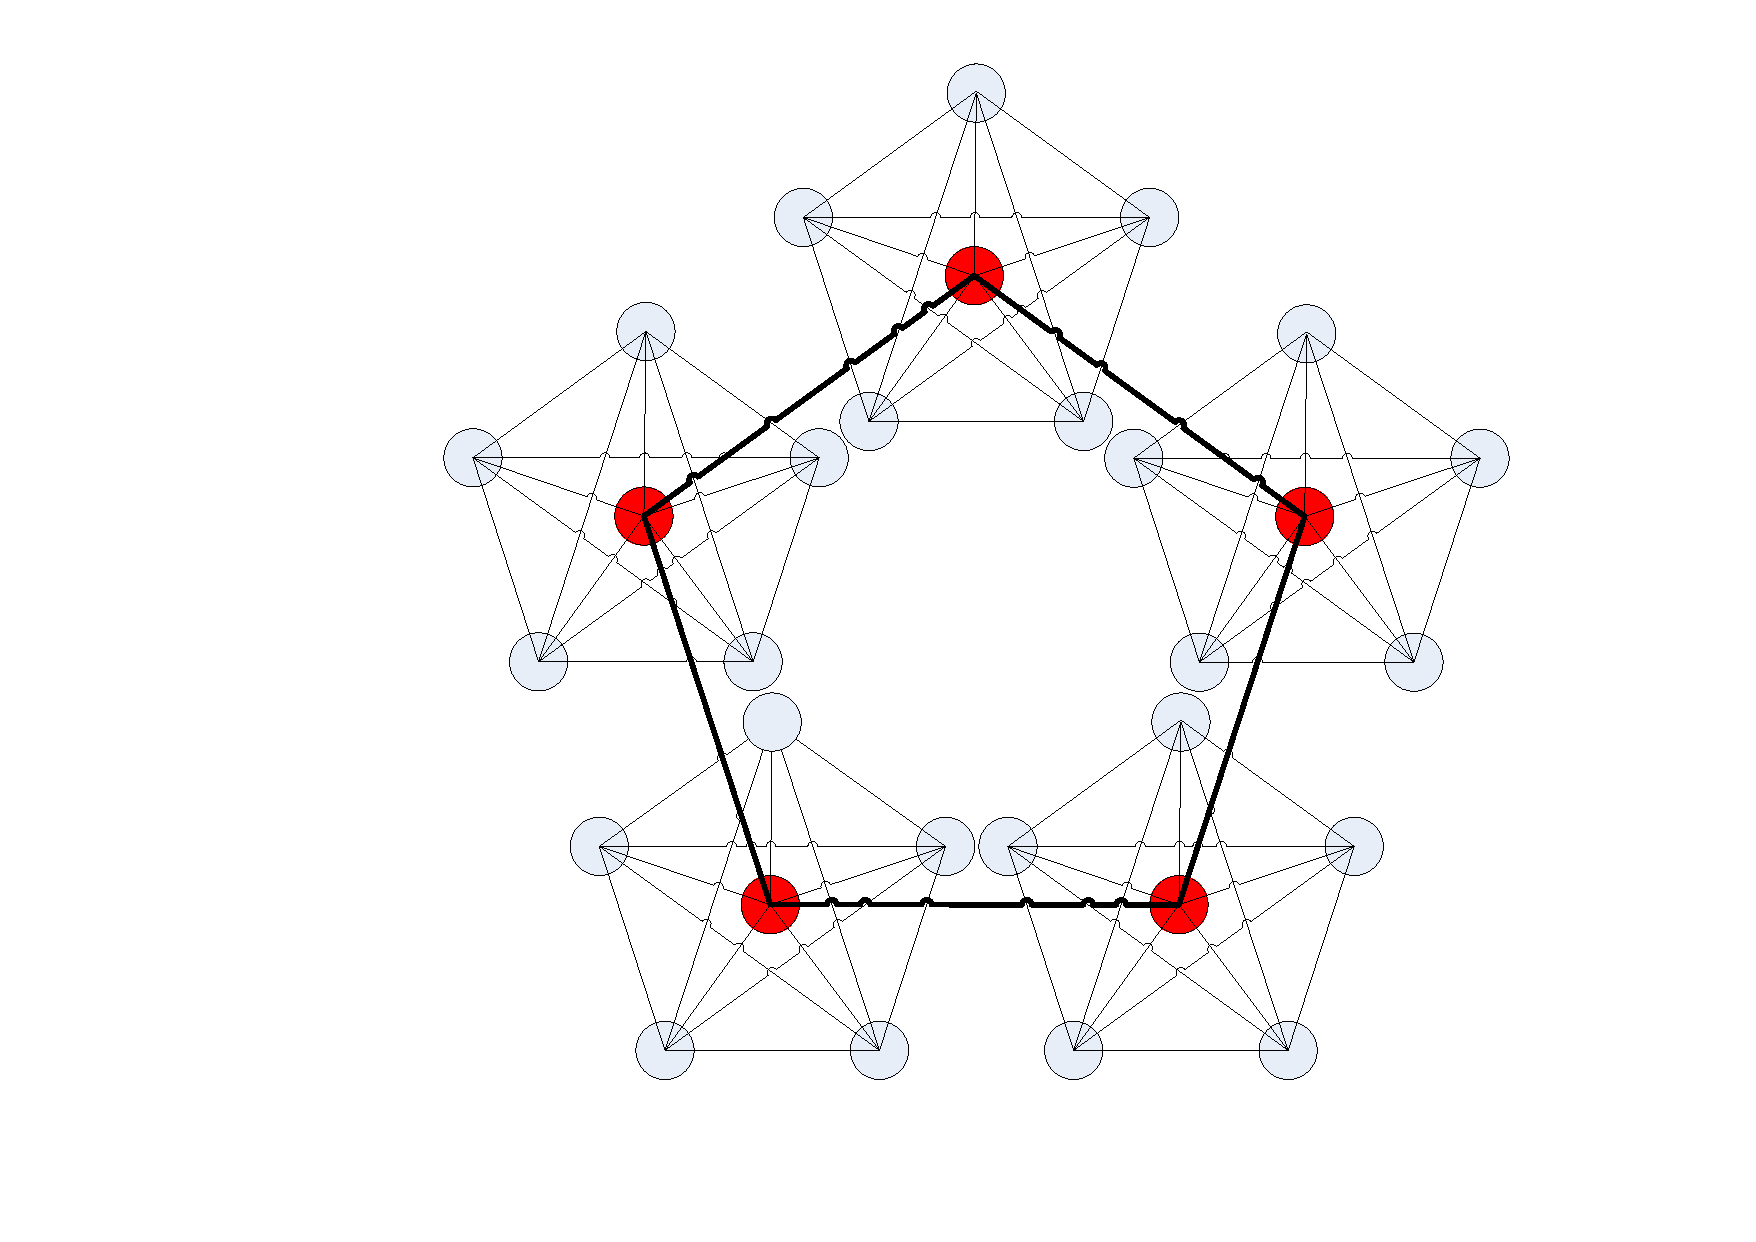
\includegraphics[clip=true, viewport=7.5cm 2.5cm 26cm 20cm, width=0.7\columnwidth]{CDHT_layout}
 \caption{Layout of the Pithos storage architecture}
 \label{fig_pithos}
\end{figure}
%
Figure \ref{fig_pithos} shows the Pithos architecture. The figure shows groups of fully connected peers (light blue and dark red), where all groups
are connected to each other in an P2P overlay through super peers (red).

Pithos groups peers to form a two tiered storage model. The first tier is a storage model at group level and the second is a storage model over all
groups. On the first tier, which is the intra-group level, a fully distributed storage system is used to allow for highly responsive read and write
operations within the group. On the second tier, which is the inter-group level, a P2P overlay is used to store data between groups.

According to categorisation of \ref{current_models}, Pithos is a type of hybrid storage, that incorporates overlay storage and distance-based
storage. Responsiveness is achieved by constructing fully connected networks amongst groups of players and then storing objects that are mostly used
by the group within the group, as described in Sections \ref{grouping}, \ref{store_retrieve} and \ref{distance_based}. Reliability is achieved by
making use of replication and migration mechanisms as described in Section \ref{store_retrieve}. Security is achieved by using a certification
authority to assign node IDs and signing any storage and retrieve request with the requesting node's certificate, as described in Section
\ref{secure_ids}. Fairness is achieved by having all nodes store objects, as described in Sections \ref{store_retrieve} and \ref{distance_based}.

\subsection{Grouping}
\label{grouping}

%Speak more concretely of grouping algorithms
At the core of the architecture is the peer clustering mechanism. Two approaches are being evaluated: distributed clustering techniques (for example
affinity propagation \cite{affinity_propagation}) and dynamic regioning techniques (for example self-organising spatial publish subscribe (SOSPS)
\cite{self_organising_sps_post}).

\emph{Distributed peer clustering techniques}: make use of the flocking behaviour of players to dynamically group players into flocks or clusters
\cite{flocking}. The main idea of flocking is that players move around in groups, rather than randomly on their own. It is desirable that user
density within groups should remain constant, because a fully distributed architecture is not scalable. This means that groups should merge or split
as the user density within them change.

Affinity propagation clusters nodes using a similarity matrix to find similar nodes. The similarity matrix may contain user positions. In this case,
affinity propagation will group nodes depending on their location in a virtual world. This algorithm is ideally suited to P2P applications, since it
is a distributed clustering algorithm based on message passing.

\emph{Dynamic regioning}: divides the virtual world into regions that can be resized or further divided to maintain constant player densities across
regions. SOSPS creates dynamic regions based on a Voronoi overlay network \cite{voronoi_diagrams_survey}. Near constant user density is achieved by
increasing and decreasing the area sizes. This system is based on VON, a distributed Voronoi overlay network designed for MMVEs \cite{VON_VAST}.

\subsection{Replication}
\label{store_retrieve}

When storing objects in Pithos, replication is used to increase object availability under network churn and for security in the presence of malicious
nodes \cite{storage_and_chaching_PAST}. For every object that is stored in Pithos, $k$ object replicas are also stored. The number of replicas ($k$)
depends on the degree of network churn as well as the number of expected malicious users in the network. If the network churn is high, more replicas
are required to avoid the situation where all $k$ peers hosting an object leaves the network before any object migration can be done.

If a node leaves the network and stops to transmit ``keep alive'' messages, the migration mechanism will detect this and replicate the file on
another node. Replication exists intra- as well as inter-group and is useful in ensuring that if a nodes leaves the network, the data are not lost.
All object requests are routed to the peer with the next closest ID if the root peer leaves, because of how overly routing functions. The new
destination peers will possess the stored files, since Pithos stores overlay replicas at overlay neighbours.

Another reason to replicate game objects is to make the system more secure. If it is known that a certain percentage of users are malicious, it is
advantages to have more replicas than malicious users. This will allow for a secure system where object hashes can be compared to determine which
nodes are malicious and what version of an object is accurate.

\subsection{Distance-based storage}
\label{distance_based}

For Pithos to succeed as an MMVE storage architecture, intra-group data requests should be preferred to inter-group data requests. This requirement,
combined with the fact that the grouping algorithm geographically groups players in the virtual world, lends Pithos to a storage system based on
distance-based storage. Similar to interest management, the assumption is that players have a limited area of interest and require interaction with a
limited number of objects within range.

Therefore, distance-based storage is implemented on a group level rather than an individual level. This means that objects are stored on the nearest
group of players, rather than the nearest user. It is assumed that such an approach will alleviate the security and reliability challenges present in
distance-based storage \cite{gilmore_p2p_mmog_state_persistency}.

With group-based distance-based storage, it is assumed that because peers now store objects closest to the group, the objects that they are
interested in will most likely be stored within their own group. Therefore, most data requests should be intra-group requests. The overlay storage
component ensures that nodes that require data, which are not stored within their group, are still able to access requested data.

\subsection{Secure storage and node ID assignments}
\label{secure_ids}

In order to design a secure distributed storage system, one requirement for the P2P overlay is that nodes should not be able to select their own IDs
or it will not be possible to secure the system against attack. Node IDs should rather be assigned securely by some certification authority
\cite{secure_overlay_routing}.

To meet this requirement, Pithos implements its own certification authority to assign node IDs securely and promote security in the P2P overlay. A
certification server exists that handle ID requests from nodes. The server assigns IDs to nodes and provides the node with a signed certificate that
it may use to store data.

Whenever an object is stored or updated in the storage network, nodes have to sign the object to enable the tracking of object changes throughout the
life of the object. This system is very different from classic distributed file storage designs that advocate anonymity in storage. The fact that all
changes can be tracked to a specific node will simplify the task of eliminating user cheating.

    \subsection{Structure}

        \subsection{DHT implementation}

    \section{Data structures}

        \subsection{Game object}

        \subsection{Group ledger}

    \section{Joining the network}

    \section{Storing data}

    \section{Retrieving data}

    \section{Modifying data}

    \section{Designing for network churn}

    \section{Group consistency}

    \section{Repair mechanisms}

    \section{Group migration}

    \section{Implementation}
    The proposed multi-tiered model is currently being implemented in Oversim \cite{OverSim_2007}, a P2P simulation environment based in Omnet++, which
allows for the measurement of identified requirements. Furthermore, it allows for the comparison of the current model with other state persistency
models. Initial results are promising, with the implemented model functioning as expected. The simulated system is very responsive when storing data
within a group and as responsive as storing data in an overlay, when storing data between groups.

Pithos is designed to form part of a complete P2P MMVE network solution. It is assumed that there exists some intelligence that drives Pithos and has
to determine when objects have to be stored and retrieved on each peer. This driving intelligence is termed the game layer.

In the results shown, Pastry was used as the P2P overlay and Pithos was driven by a \emph{Game} module developed for this purpose. After a node has
joined a group, the game module starts to generate store and retrieve requests at a rate of 10 objects per second and a size of 1024 bytes. The size
of 1024 byte objects was chosen to be much larger than Quake 3 game objects without delta encoding, used in \cite{Bharambe_Donnybrook}. Pithos is
designed for the low latency storage of small game objects.

For the results shown, 14499 peers, 500 super peers and a single directory server are created at the start of the simulation. The directory server
publishes super peer information, which allows a peer to join the group nearest to it. Because of the way Pithos is structured, each super peer node
is also a peer node, which gives a total of 15000 Oversim nodes.

To be able to simulate Pithos for 15000 nodes, it runs on the Oversim simple underlay network \cite{oversim_applications}, where node latencies are
determined by the distance between nodes placed in an $n$-dimensional Euclidean space. The positions of the nodes are chosen to match the latencies
of the CAIDA/Skitter project. Different nodes are also assigned different bandwidth and jitter parameters to simulate a heterogenous network.

\chapter{State Management Parameter Modelling}
\label{chp:MODELLING}

    %%%%%%%%%%%%%%%%%%%%%%%%%%%%%%%%%%%%%%%%%%%%%%%%%%%%%%%%%%%%%%%%%%%%%%%
\section{Reliability}
\subsection{Background and related work}
\label{related_work}

To increase the time an object is available within the distributed storage system, two techniques are used: redundancy and repair. In storage systems using replication as redundancy technique, $R$ replicas of every object are stored. The number of required replicas $R$ is a design decision, the effect of which will be shown in Section \ref{results}. When all nodes containing an object's replicas have left the network, the object is no longer available. Periodic repair, which occurs at a rate of $\mu = 1/T_{\textrm{repair}}$, replaces all missing replicas.

This paper mainly extends and improves upon the work by Wu, Tian and Ng \cite{replication_article}. The related work models three characteristics of distributed hash table (DHT) lookups under churn: expected lookup latency of various routing schemes, expected lookup overhead of various routing schemes and expected object lifetime. Our paper focuses on the object lifetime characteristic. Wu, Tian and Ng develop two models for object lifetime when exponentially distributed node lifetimes are assumed. One for the case without object repair and one for the case with object repair. Node residual lifetimes are used when calculating expected object lifetimes without repair. In this case object lifetimes are equal to the maximum residual lifetime of the nodes the objects were replicated on.

%What about Pareto lifetimes?

A continuous time Markov chain, shown in Figure \ref{fig_other_markov_chain}, is used to model the expected object lifetimes for the case with repair.
%
\begin{figure}[htbp]
 \centering
 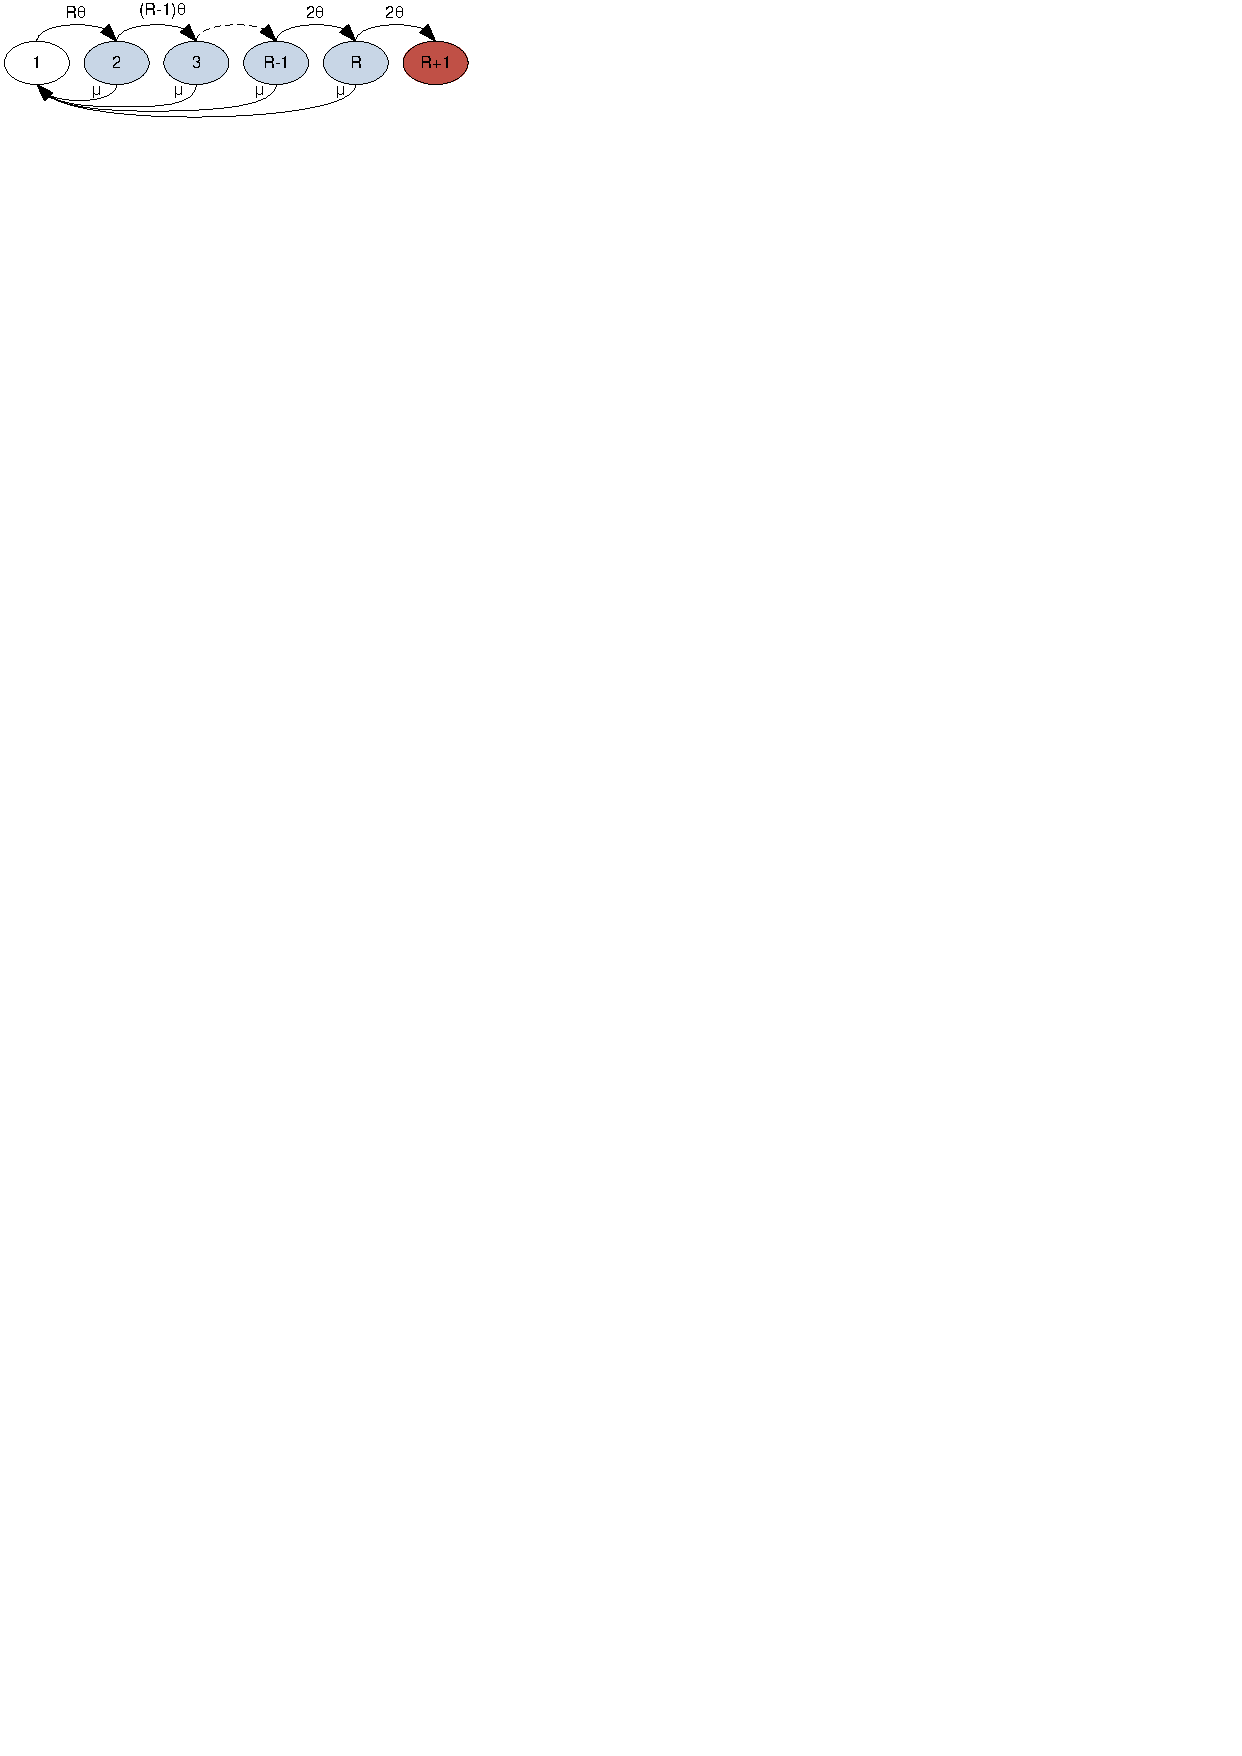
\includegraphics[clip=true, viewport=0.0cm 27.5cm 8.0cm 30.0cm, width=0.7\columnwidth]{inifinite_network_chain}
 \caption{Markov chain modeling object replica number for an infinite network size}
 \label{fig_other_markov_chain}
\end{figure}
%
The model has $R+1$ states and is in state $k$ when $R+1-k$ replicas are alive in the network. The system is, therefore, in state $1$ when all replicas are present and in state $R+1$ when no replicas are present. The authors assume that all objects are inserted into the network with $R$ replicas, i.e. enter the network in state 1. This initial state is colored white in Figure \ref{fig_other_markov_chain}. If the node departure rate under steady state is $\theta$ and there are $r$ replicas present in the network, the replica departure rate under steady state is $r\theta$. When all replicas are lost, the chain enters state $R+1$ (coloured dark) and is said to be ``absorbed''.

Our paper improves on the work by Wu, Tian and Ng \cite{replication_article} in two ways: firstly, the model is extended to take into account a finite network size. The fact that there might not be sufficient nodes to replicate the data on when objects are stored or when the repair mechanism activates. Secondly, our model unifies the cases with and without repair, to produce a single model where the effects of both might be evaluated. When our model is used with larger average network sizes, expected object lifetimes converge to those shown in the work by Wu, Tian and Ng, using their two separate models.

Predicting object lifetimes in a distributed storage system is grounded in reliability engineering theory. When network size is ignored, it is similar to predicting the mean time to failure (MTTF) of a set of parallel components with repair. Chun et al. \cite{Chun:2006_replica_maintenance} also uses a Markov chain to model object replicas with network churn and repair. They use a birth-death process similar to the model by Wu, Tian and Ng, but using incremental, instead of complete repair.

No literature could be found in general reliability engineering or distributed systems reliability research that deals with object lifetimes with finite network sizes.

\subsection{The model}
\label{model}

In order to model the effects of a finite network size on the lifetime of an object, the continuous time Markov chain model introduced in Section \ref{related_work} is expanded by adding a second parameter to every state, namely the network size. This effectively adds another dimension to the Markov chain. The resulting Markov chain is shown in Figure \ref{fig_markov_chain}.

\begin{figure}[htbp]
 \centering
 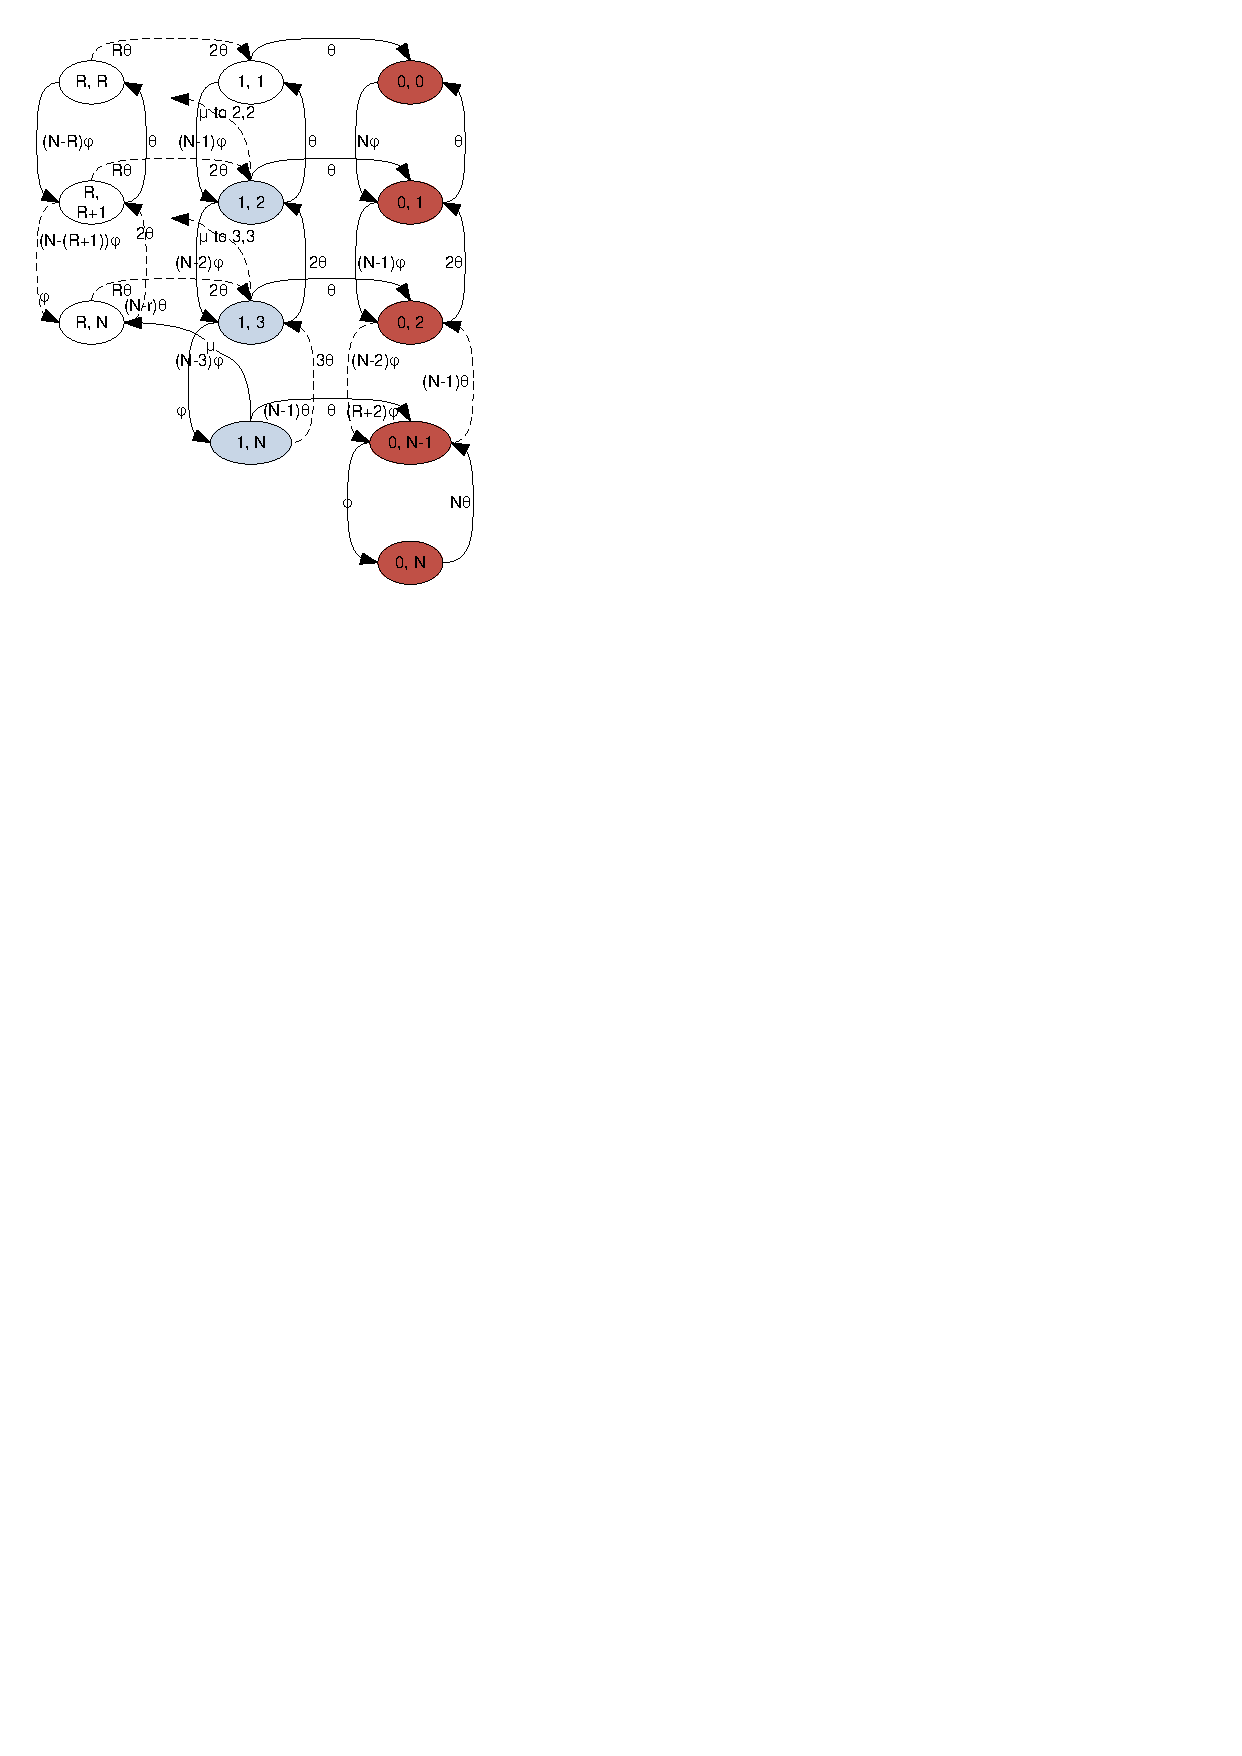
\includegraphics[clip=true, viewport=0.5cm 19.5cm 8.5cm 29.5cm, width=0.7\columnwidth]{Markov_chain_repair_compact}
 \caption{Markov chain modeling object replica number as well as network size}
 \label{fig_markov_chain}
\end{figure}

%Explain transient and absorbtion states here somewhere.

The dual parameter states can be seen in the Markov chain in Figure \ref{fig_markov_chain}. Every state is a tuple of the form \verb.(replicas,nodes).. Where $R$ is the required number of object replicas and $N$ is the maximum number of nodes in the network. It is assumed that $R$ replicas are always stored in the network, if sufficient space is available. If the number of nodes currently in the network $n$ are fewer than the required number of replicas ($n < R$), only $n$ replicas are stored. The initial states of the Markov chain are therefore all the states ($R,n$) as well as all the states ($n,n$), for $n < R$. There are therefore $N$ initial states, one for every possible network size. The initial state is the initial network size that an object is placed in.

If there are no more replicas in the network, an object cannot be repaired and the Markov chains remains in the set of states ($0,n$). These are said to be the absorbing states of the Markov chain and there exists $N - R + 1$ absorbing states in the model presented here. All other states out of which transition is possible are said to be transient states. It can be shown that if sets of transient and absorbing states exist, the system will always end up in the absorbing states \cite{grinstead1997introduction_probability}. The time to absorbtion can be calculated, which in the case of object storage means the time when no more objects exist in the network.

\subsubsection{State transition rates}

There are four types of state transitions possible in the Markov model presented here:
%
\begin{enumerate}
\item A node that contains a replica departs the network.
\item A node that does not contain a replica departs the network.
\item A node joins the network.
\item An object is repaired.
\end{enumerate}

%In a continous Markov chain we define delta small enough so only one event can occur at any point in time

\begin{figure}[htbp]
 \centering
 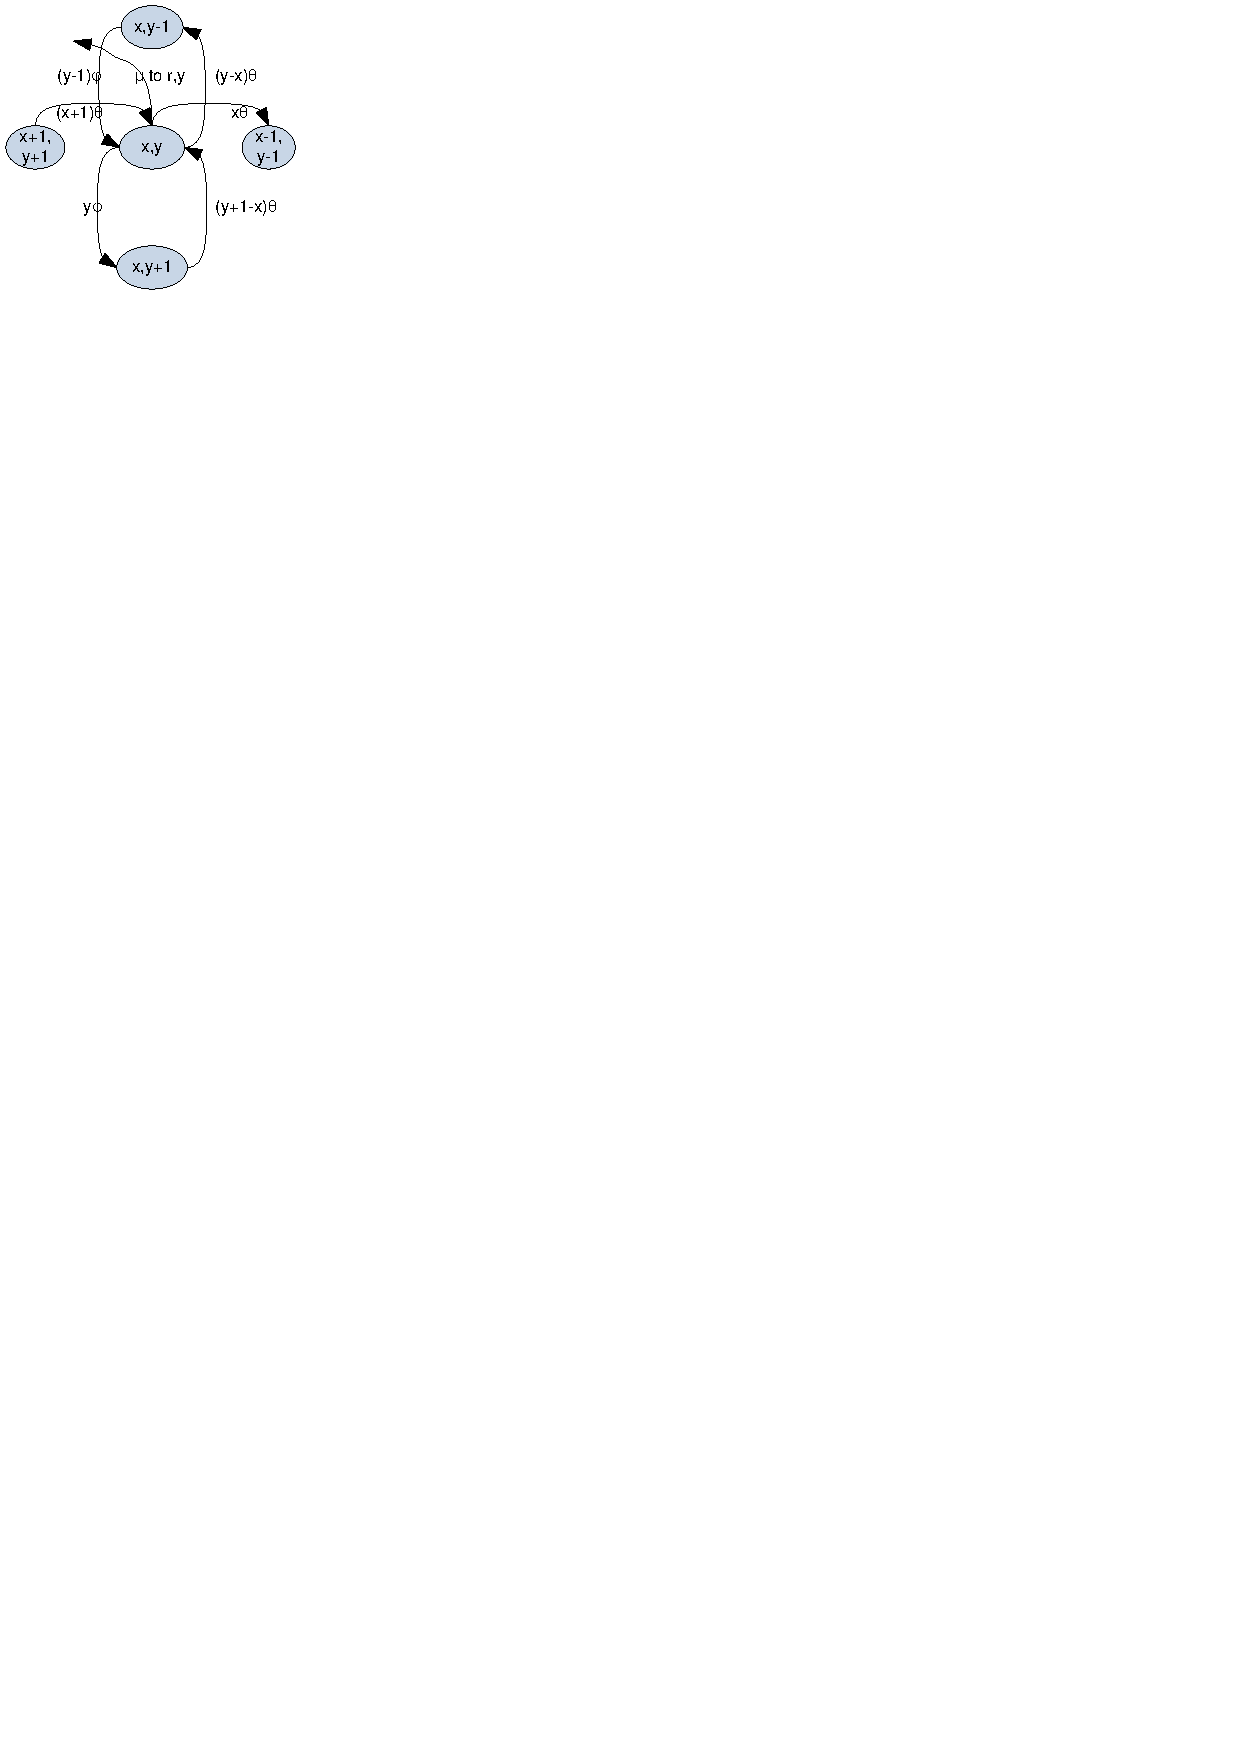
\includegraphics[clip=true, viewport=0.0cm 24.5cm 5.0cm 30cm, width=0.6\columnwidth]{Markov_example}
 \caption{Markov chain modeling object replica number as well as network size}
 \label{fig_markov_example}
\end{figure}

State transitions can be explained by the example in Figure \ref{fig_markov_example}. The figure shows all state transitions relative to the centre state ($i,k$). For the purposes of explanation, only transitions to and from the centre state are shown. Starting at state ($i+1,k+1$), where $i+1$ replicas and $k+1$ nodes are present. If a node that contains a replica departs the network, the system moves to state ($i,k$): one fewer replica and one fewer node.

If a node that does not contain a replica now departs from the network, the system moves from state ($i,k$) to ($i,k-1$): no fewer replicas and one fewer node. A node can join the network, which will have the model move from ($i,k-1$) to ($i,k$) and another node joining the network will move the system into state ($i,k+1$).

The periodic repair mechanism, introduced in Section \ref{related_work} is also present. With sufficient nodes available for a full repair, the system moves from state ($i,k$) to ($R,k$). When the network size is smaller than the required number of replicas, the system moves to state ($N,k$) instead.

For dual states, state transition rates are characterised by moving from state $i k$ to state $j l$, where $i$ is the number of replicas in the current state, $k$ the number of nodes in the current state, $j$ the number of replicas in the next state, and $l$ the number of nodes in the next state. Every state transition rate can then be expressed as a dual state transition equation.

Let $\theta$ be the departure rate of nodes under steady state. For a current state of $i$ replicas, the departure rate of nodes containing replicas from the network is $i\theta$. This transition can be expressed in terms of the dual state transition equation:
%
\begin{equation} \label{eq_rep_left}
    p(i k,j l)_{(\textrm{replica left})} = i\theta,\quad\textrm{for}\quad j = i - 1,\quad l = k - 1,
\end{equation}
%
where the next state contains one fewer replica and one fewer node than the current state.

The departure rate of nodes not containing replicas is the difference between the number of nodes currently in the network $k$ and the number of replicas currently in the network $i$. The departure rate is then $(k - i)\theta$ and the transition is given by
%
\begin{equation} \label{eq_node_left}
    p(i k,j l)_{(\textrm{node left})} = (k - i)\theta,\quad\textrm{for}\quad j = i,\quad l = k - 1,
\end{equation}
%
where the next state contains one fewer node, but the same number of replicas as the current state.

The Markov model assumes the presence of a finite sized network, with some maximum number of nodes $N$. Let $\phi$ be the arrival rate of peers under steady state. The departure rate of nodes from the network is dependant on the number of nodes in the network. Similarly, if a maximum network size is assumed, the arrival rate of nodes in the network can be modelled as a function of nodes \emph{not} in the network. This creates a symmetry between the network departure and arrival rates, which creates a ``force'' in the Markov model that pushes the network to some average network size, which is a ratio of $\theta$ to $\phi$. A stationary average network size is required to model a steady state network.

The arrival rate of nodes can thus be modelled as $(N - k)\phi$, the product of a single node arrival rate and the number of nodes not currently in the network, as given by
%
\begin{equation} \label{eq_node_arrived}
    p(i k,j l)_{(\textrm{node arrived})} = (N - k)\phi,\quad\textrm{for}\quad j = i,\quad l = k + 1,
\end{equation}
%
where the next state contains one more node, but the same number of replicas as the current state.

%Perhaps add some graphs here to show how node departure and arrival rate change with changes in network size. Show a graph or equation that will show the trend towards a single average. Perhaps use something like the rate difference to show force towards the centre.

$N$ should be chosen sufficiently large, compared to the average network size $\tilde{n}$, to ensure that the probability of the network model ever reaching $N$ is vanishingly small. What constitutes a sufficiently large maximum network size will be evident from the results presented in Section \ref{results}. This requires that the ratios of $\theta$ to $\phi$ be chosen to produce a network with an average network size much smaller than $N$.

For the network to be in steady state, the mean arrival rate of nodes must equal the mean departure rate of nodes, which gives
%
\begin{equation}
    (N - \tilde{n})\phi = \tilde{n}\theta.\label{eq_phi_theta_ratio}
\end{equation}

Making $\phi$ the subject of Equation \eqref{eq_phi_theta_ratio} gives
%
\begin{equation}
    \phi = \frac{\tilde{n}\theta}{N - \tilde{n}},\label{eq_phi}
\end{equation}
%
which provides a value for $\phi$ that will produce a network with the desired average network size $\tilde{n}$, for a given $\theta$ and $N$.

It is assumed that the repair mechanism repairs objects once every $T_{\textrm{repair}}$ time or at a rate of $\mu = 1/T_{\textrm{repair}}$, which gives
%
\begin{equation} \label{eq_repair}
    p(i k,j l)_{(\textrm{repair})} = \mu,\quad\textrm{for}\quad j = \min(R, l),\quad l = k,\quad i \neq j.
\end{equation}
%
The number of replicas in the next state is either equal to the required number of replicas or the current number of nodes, whichever one is smallest, and the number of nodes remain the same as in the current state. When no replicas are missing, no repair occurs.

No transitions other than the ones described above can occur in the presented Markov model, therefore $p(i k,j l) = 0$ for all other state transitions.

\subsubsection{Node departure rate}

The node departure rate $\theta$ can be calculated from the lifetime distributions of the nodes in the network. As in the related work discussed in Section \ref{related_work}, all node lifetimes are assumed to be statistically independent and exponentially distributed. The exponential distribution is characterised by the single ``rate'' parameter $\lambda$.

The departure rate of nodes correspond to the failure rate (also called the hazard rate) of the node lifetime distribution \cite{rausand2004systemreliability}. An advantage of the exponential distribution is its ``memoryless'' property, which has a constant failure rate $h = \lambda$. For nodes with exponential lifetime distributions, the node departure rate is therefore $\theta = \lambda$.

\subsubsection{Number of states}

The Markov model presented in this paper possesses a large number of states. To calculate the total number of states, two cases are identified. The first case is where the number of nodes in the network is greater or equal to the required number of replicas $k \geq R$. For every possible network size in this group, there are $R$ states and $N - R + 1$ possible network sizes. From this it is evident that there are $(N - R + 1)R$ of these states.

The second case is where the number of nodes in the network is fewer than the required number of replicas. For every possible network size in this case, the number of states are equal to the number of nodes in the network, going from $R-1$ to 1.

The total number of states is the sum the two cases and given by
%
\begin{align}
       S & = R(N - R + 1) + \sum_{x=1}^{R-1} x\label{eq_states_num_init}\\
         & = R(N - R + 1) + 0.5 (R - 1) R\notag\\
         & = 0.5 R (2 N - R + 1), \quad\textrm{where}\quad N \geq R. \label{eq_states_num_ans}
\end{align}

If a small network of 500 nodes with objects each having 10 replicas is modeled, the resulting Markov chain contains 4955 states. The large number of states makes a closed form solution to the object lifetime problem intractable. Fortunately, numerical methods can be used to calculate object lifetimes for given numbers of replicas and maximum node sizes.

\subsubsection{Calculating object lifetimes}

Since each element in the transitional rates matrix is a rate, the sum of all the elements in a single row of the rates matrix gives the rate of moving from that state to any other state. The inverse of this rate is the expected time $t_i$ the Markov chain spends in state $i$, given by
%
\begin{equation} \label{eq_markov_rates}
    t_i = \left(\sum_{j} p_{i, j}\right)^{-1}.
\end{equation}

In a embedded Markov chain, the sum of all rows in the transitional rates matrix must equal one. This is achieved by normalising each row in the transitional rates matrix \textbf{P} to produce the normalised transitional rates matrix \textbf{\^{P}}, where each row in the matrix must satisfy
%
\begin{equation} \label{eq_markov_sum}
    \sum_{j} \hat{p}_{i, j} = 1.
\end{equation}

Using $t_i$, the expected time spent in state $i$, \textbf{\^{P}} is given by
%
\begin{equation} \label{eq_markov_normalisation}
    \hat{p}_{i, j} = p_{i, j} t_i.
\end{equation}

Object lifetime can be calculated by calculating the expected time to absorbtion of the embedded continuous time Markov chain. To do this, the normalised transitional rates matrix is partitioned into the form
%
\begin{equation} \label{matrix_partition}
    \textbf{\^{P}} = \left[\begin{array}{c|c}
                   \textbf{Q} & \textbf{R} \\
                   \hline
                   \textbf{0} & \textbf{I}
                 \end{array}\right].
\end{equation}
%
Every state transition can be considered a discrete event, which allows for the continuous time Markov chain to be embedded. This allows for theory from discrete time Markov chains to be used, with the exception that events are not equally spaced in time.

\textbf{\^{P}} is partitioned in such a way that all absorbing states are in the last rows and columns of \textbf{\^{P}}. Suppose there are $a$ absorbing states and $\tau$ transient states in the model. The matrix \textbf{Q} is then a $\tau\times\tau$ sub-matrix of \textbf{\^{P}} that contains all transient states. \textbf{I} is an $a \times a$ identity matrix, \textbf{0} is a $a\times\tau$ zero matrix and \textbf{R} (not to be confused with $R$) is a nonzero $\tau\times a$ matrix.

From \textbf{Q}, the fundamental matrix \textbf{N} may be calculated as \cite{grinstead1997introduction_probability}
%
\begin{equation} \label{eq_fundamental_mat}
    \textbf{N} = (\textbf{I} - \textbf{Q})^{-1}.
\end{equation}
%
Every element $n_{x,y}$ in the fundamental matrix \textbf{N} gives the expected number of times that the model is in the state $y$, if it started in the transient state $x$.

The expected time to absorbtion is then the product of the time spent in each state and the expected number of times a state will be entered, as given by
%
\begin{equation} \label{expected_lifetime}
    \textbf{E[L]} = \textbf{Nt},
\end{equation}
%
where \textbf{t} is the vector consisting of the times $t_i$ for all $i$.

\subsection{Model results}
\label{results}

For all results presented in this section, the following parameter values are used: a maximum network size of $N=120$, a required number of replicas of $R = 10$ and exponential node lifetime distributions with $\lambda = \theta = 1/1800$, which gives expected \emph{node} lifetimes of $1/\lambda = 1800$ seconds.

%Maybe explain where these values come from or why the were used.

\begin{figure}[htbp]
 \centering
 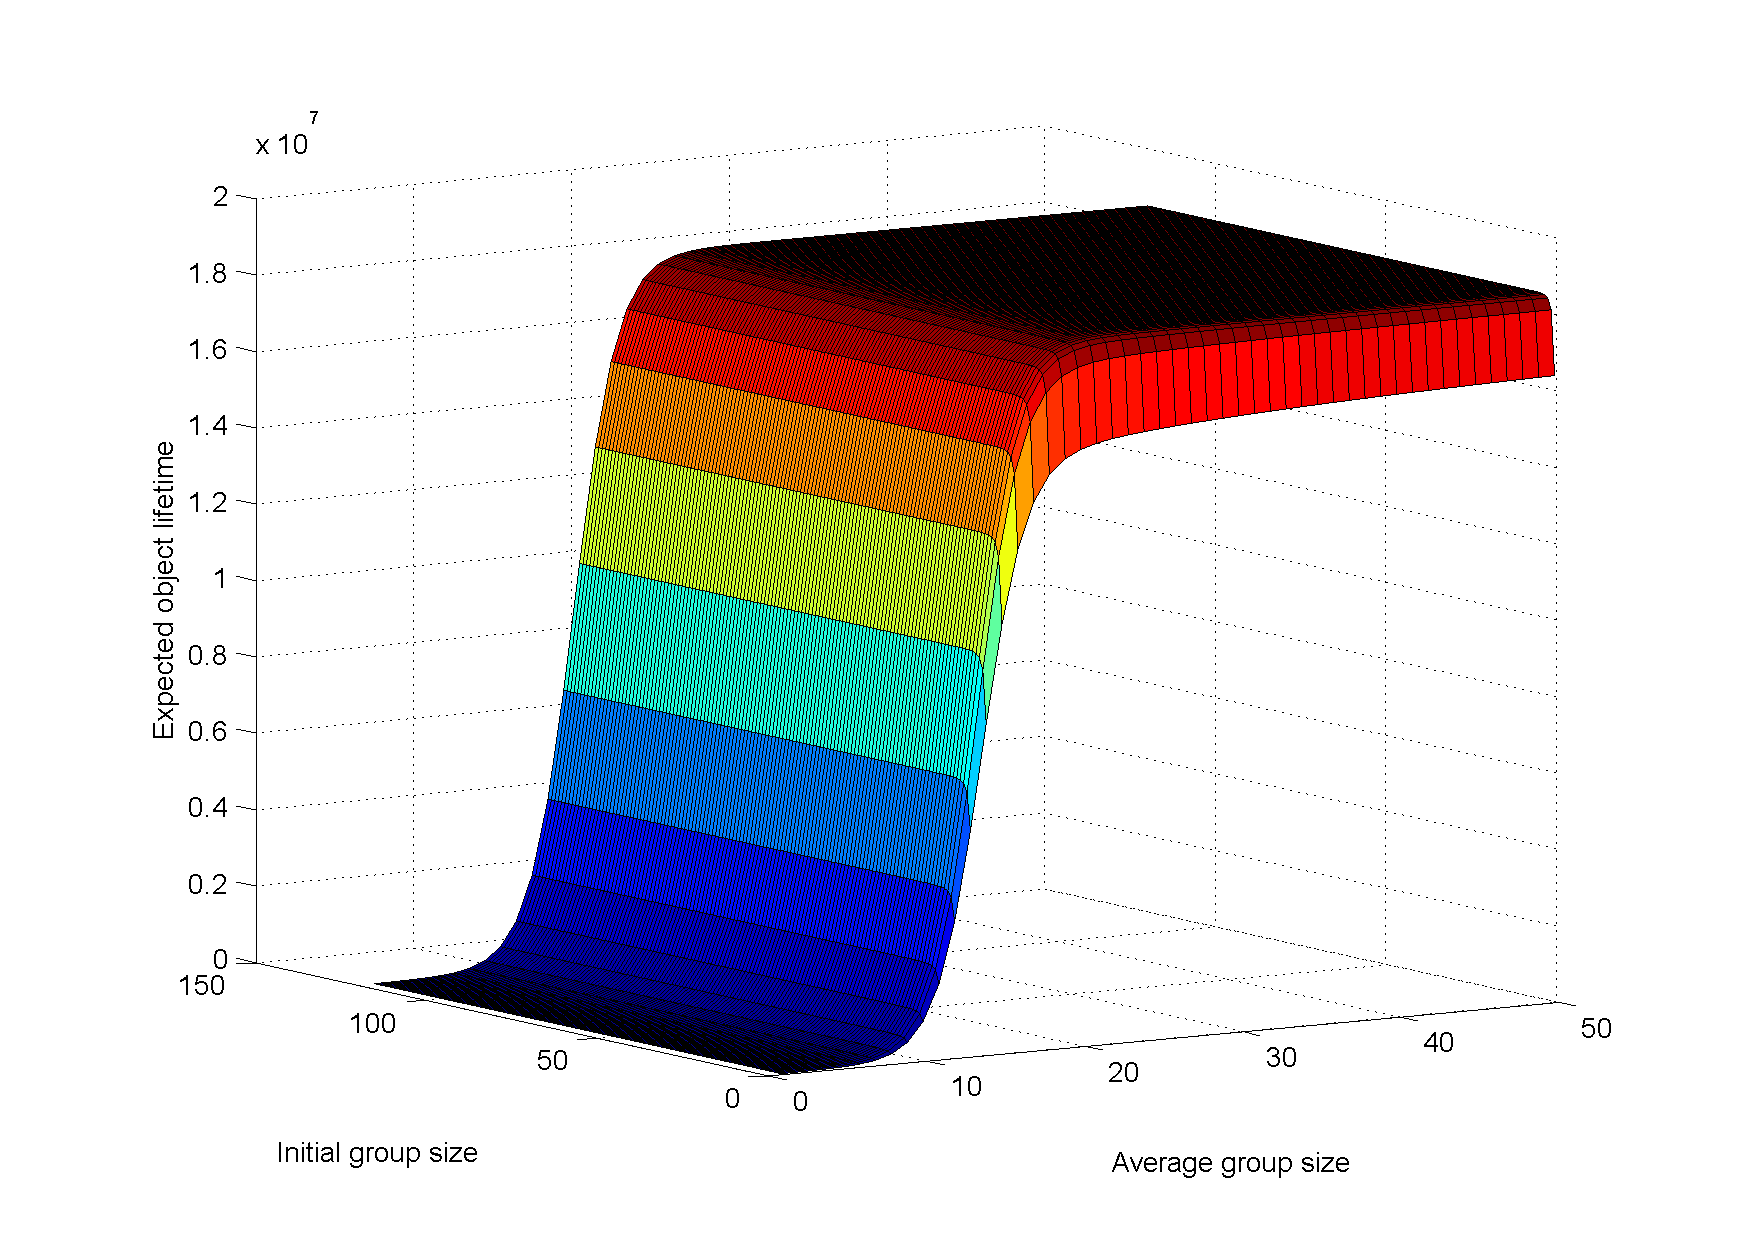
\includegraphics[clip=true, viewport=1.5cm 3.5cm 28.0cm 16.5cm, width=\columnwidth]{lifetime_av_init_groupsize}
 \caption{Surface plots of expected object lifetimes as functions of initial and average network sizes for $\mu = 1/180$ (above) and $\mu = 0$ (below).}
 \label{fig_lifetime_average_vs_initial}
\end{figure}
%
Figure \ref{fig_lifetime_average_vs_initial} shows surface plots of expected object lifetimes against initial and average network sizes for a repair rate of $\mu = 1/180$ (or $T_{\textrm{repair}}$ $10\%$ of the expected node lifetime) and no repair rate. It is evident that object lifetimes decrease greatly for average network sizes smaller than 20 nodes for the case with repair, but that average network size has no effect when repair is not used. The model presented in this paper shows a significant decrease in expected lifetime every time the average network size is comparable to the required number of replicas, for the case with repair. The figure also shows that expected object lifetimes decrease when the initial network size is smaller than the required number of replicas. From the figure it can also be seen that initial network size has a more pronounced effect on the expected object lifetime, when no repair is used than when repair is used.

\begin{figure}[htbp]
 \centering
 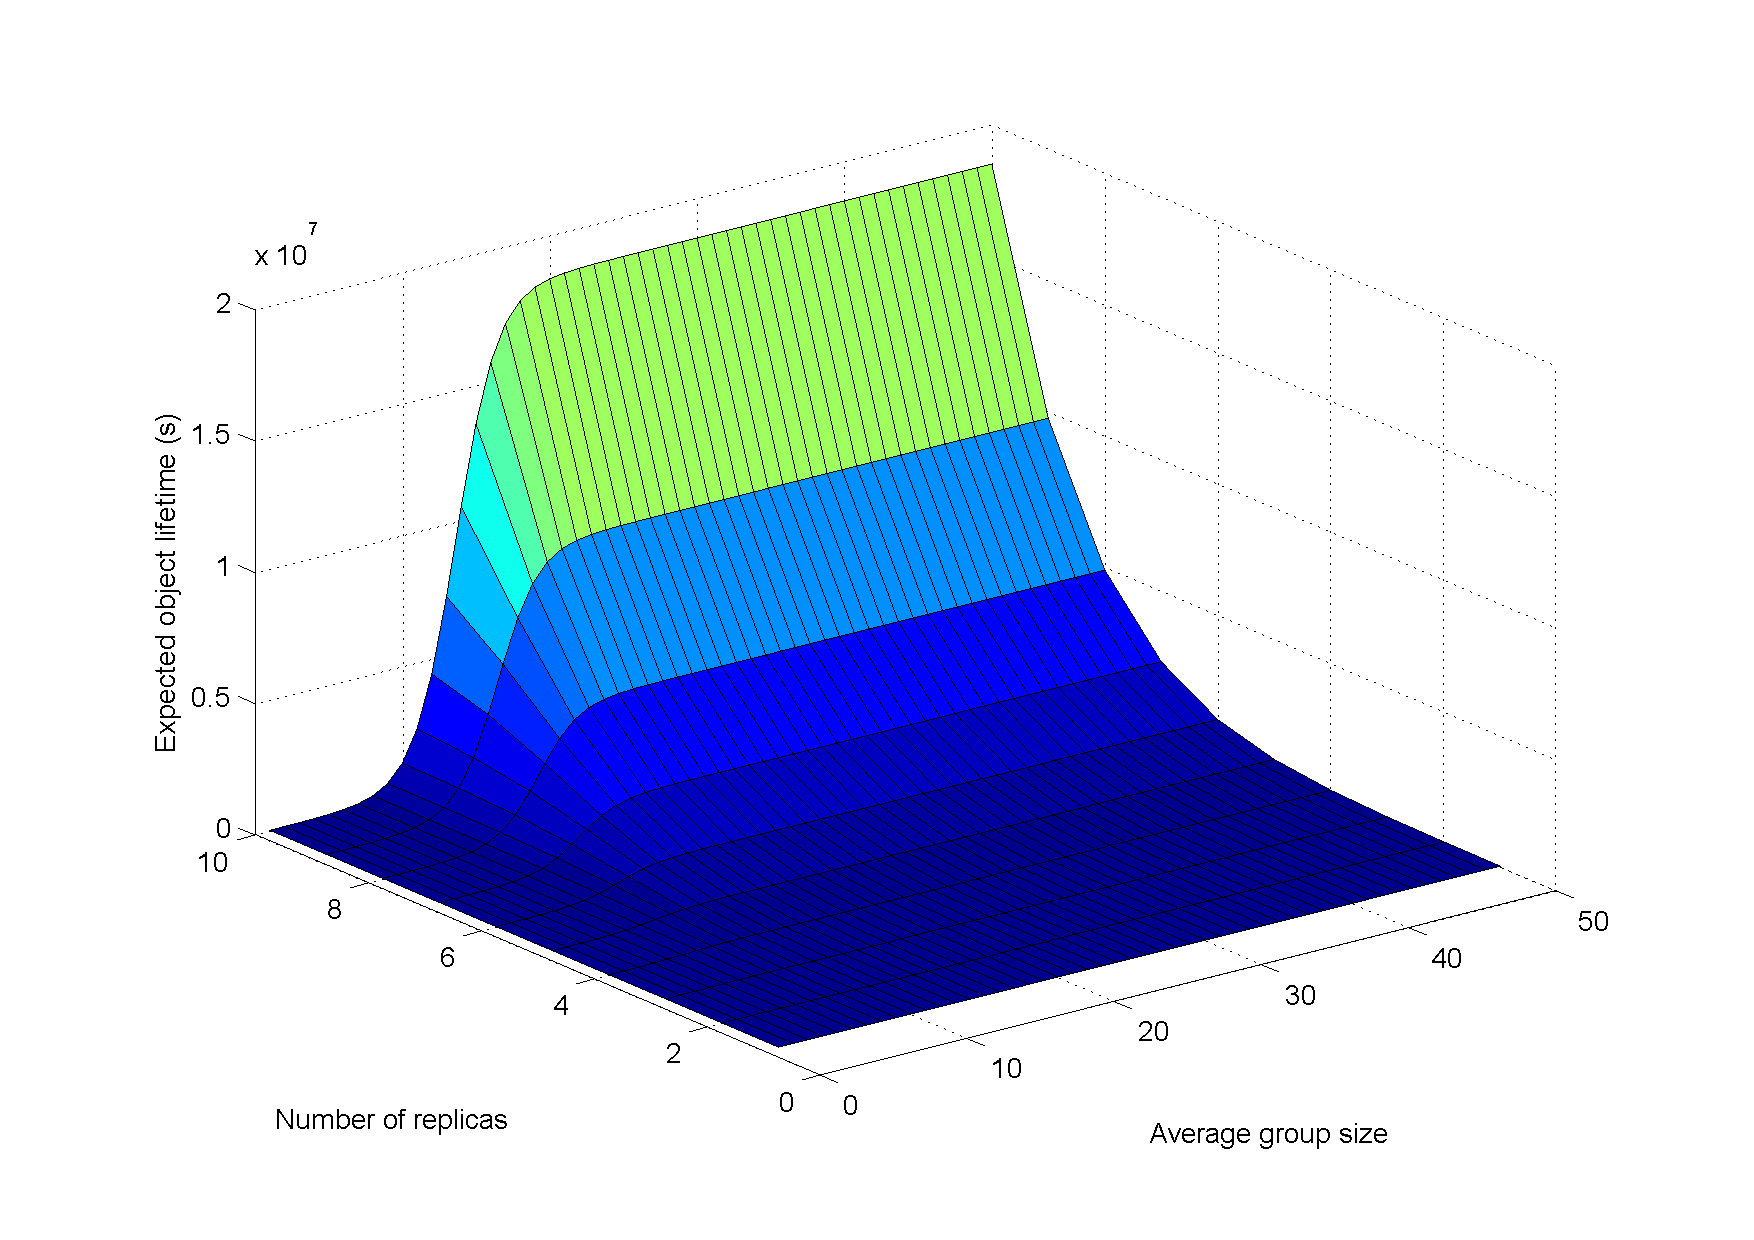
\includegraphics[clip=true, viewport=2.5cm 1.0cm 27.5cm 19.15cm, width=0.8\columnwidth]{lifetime_replicas_av_groupsize}
 \caption{Surface plot of expected object lifetimes as functions of average network size and required number of replicas $R$ for $mu = 1/180$.}
 \label{fig_lifetime_average_vs_replicas}
\end{figure}
%
Figure \ref{fig_lifetime_average_vs_replicas} depicts the expected object lifetime as functions of average network size and required number of replicas $R$ for a repair rate of $\mu = 1/180$. To generate this figure, $R$ is swept from 1 to 10 to illustrate the effect that an increase in the number of replicas has on the expected node lifetime. The figure shows that an increase in $R$ leads to an exponential increase in the expected object lifetime, but that this gain is limited when the average network size is small, compared to the required number of replicas.

\begin{figure}[htbp]
 \centering
 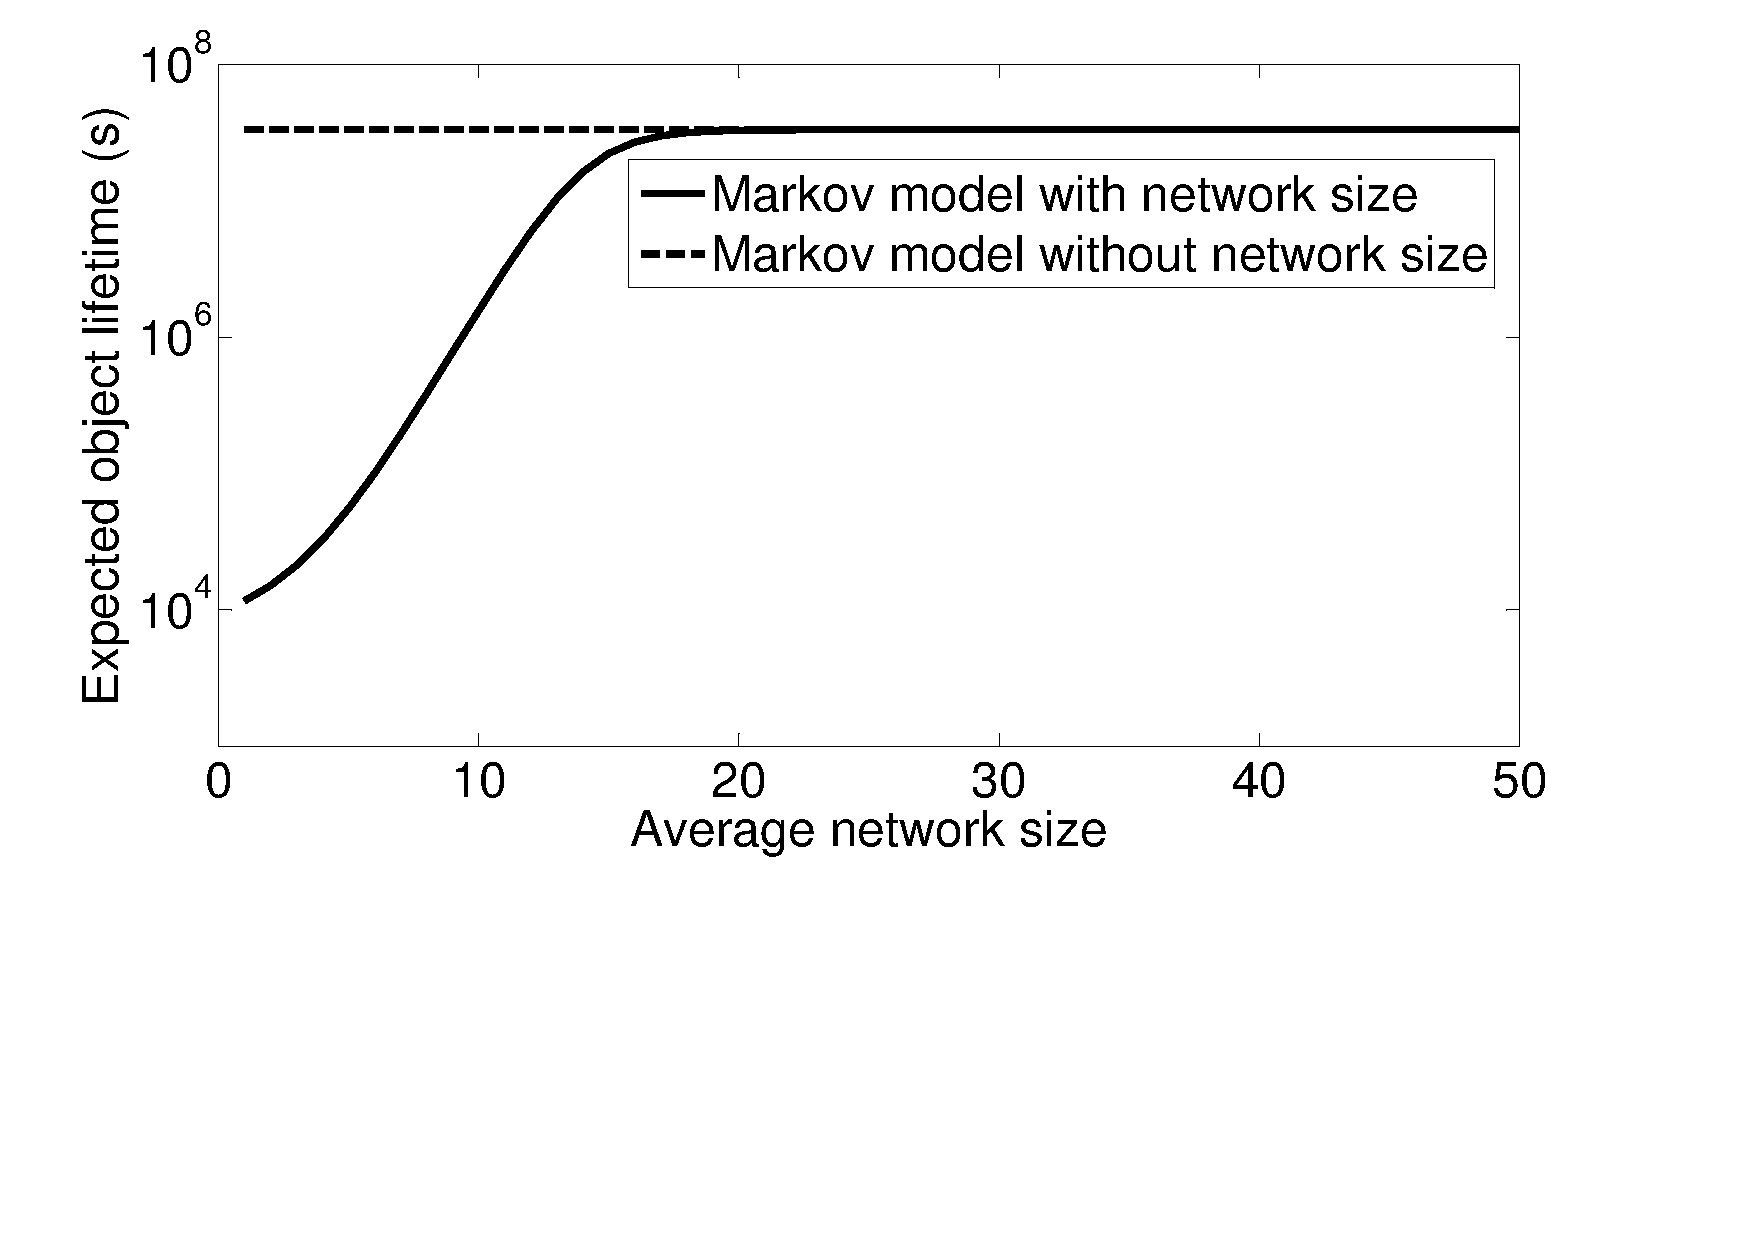
\includegraphics[clip=true, viewport=1.0cm 6.5cm 26.5cm 20.5cm, width=0.8\columnwidth]{lifetime_av_models_compare}
 \caption{Surface plot of expected object lifetimes as functions of initial and average group sizes.}
 \label{fig_lifetime_vs_other_model}
\end{figure}

Figure \ref{fig_lifetime_vs_other_model} compares the model presented in this paper with the model of Wu, Tian and Ng that assumes object repair \cite{replication_article}. For this figure, a repair rate of $\mu = 1/180$ and a required number of replicas of $R = 10$ were used. As shown, because the model by Wu, Tian and Ng does not take average network size into account (or initial network size for that matter) it cannot predict the object lifetimes correctly for average network sizes comparable to the required number of replicas. On the other hand, a reliability test of the model presented in this paper is that for sufficiently large network sizes, the model converges to the model that assumes an infinite network size.

\subsection{Comparison with Pithos simulation}
\label{simulation}

To determine practical usability of the theoretical results presented in Section \ref{results}, a comparison was performed against the Pithos simulation \cite{Pithos_mmve_2011}. Pithos is a hierarchical distributed storage system that uses grouping to reduce latencies of store and retrieve requests, as is required by massively multiuser virtual environments (MMVEs) \cite{gilmore_p2p_mmog_state_persistency}.

The Oversim environment contains churn generators that create \emph{peers} with lifetimes sampled from an exponential distribution. A single \emph{super peer} was also created and never destroyed. Super peers allow new nodes to join the group by working with the dedicated \emph{directory server} for network bootstrapping. A single group was used, because multiple groups have different average group sizes during different simulations, which reduces the number of measurements per average group size to below statistical significance.

During a simulation run, the Pithos test application generates random objects and require these objects to be stored in the network. Every node only generated objects for a specified amount of time. This is done to limit the total number of objects present in the system to a few hundred thousand. For numbers larger than this, the simulation would run out of memory and grind to a halt. To allow simulation of the case of long lived objects, the Pithos simulation was deployed on a ``High-Memory Quadruple Extra Large Instance'' in the Amazon EC2 cloud, which contains 68.4 GB of RAM.

``Box and whiskers plots'' are used to compare the simulation data with the theoretical model. This allows for comparisons of mean values, but also shows how the data are distributed. In the box plot, the black striped whiskers show the minima and maxima of the data sets. The lower and upper bounds of the boxes show the 25th and 75th percentiles respectively. The horizontal lines in the boxes show the medians of the data, and the ``notches'' around the medians show the 5\% significance levels. The cross present in every box shows the simulation data mean and the solid line running through the boxes shows expected object lifetimes as predicted by the theoretical model.

\begin{figure}[htbp]
 \centering
 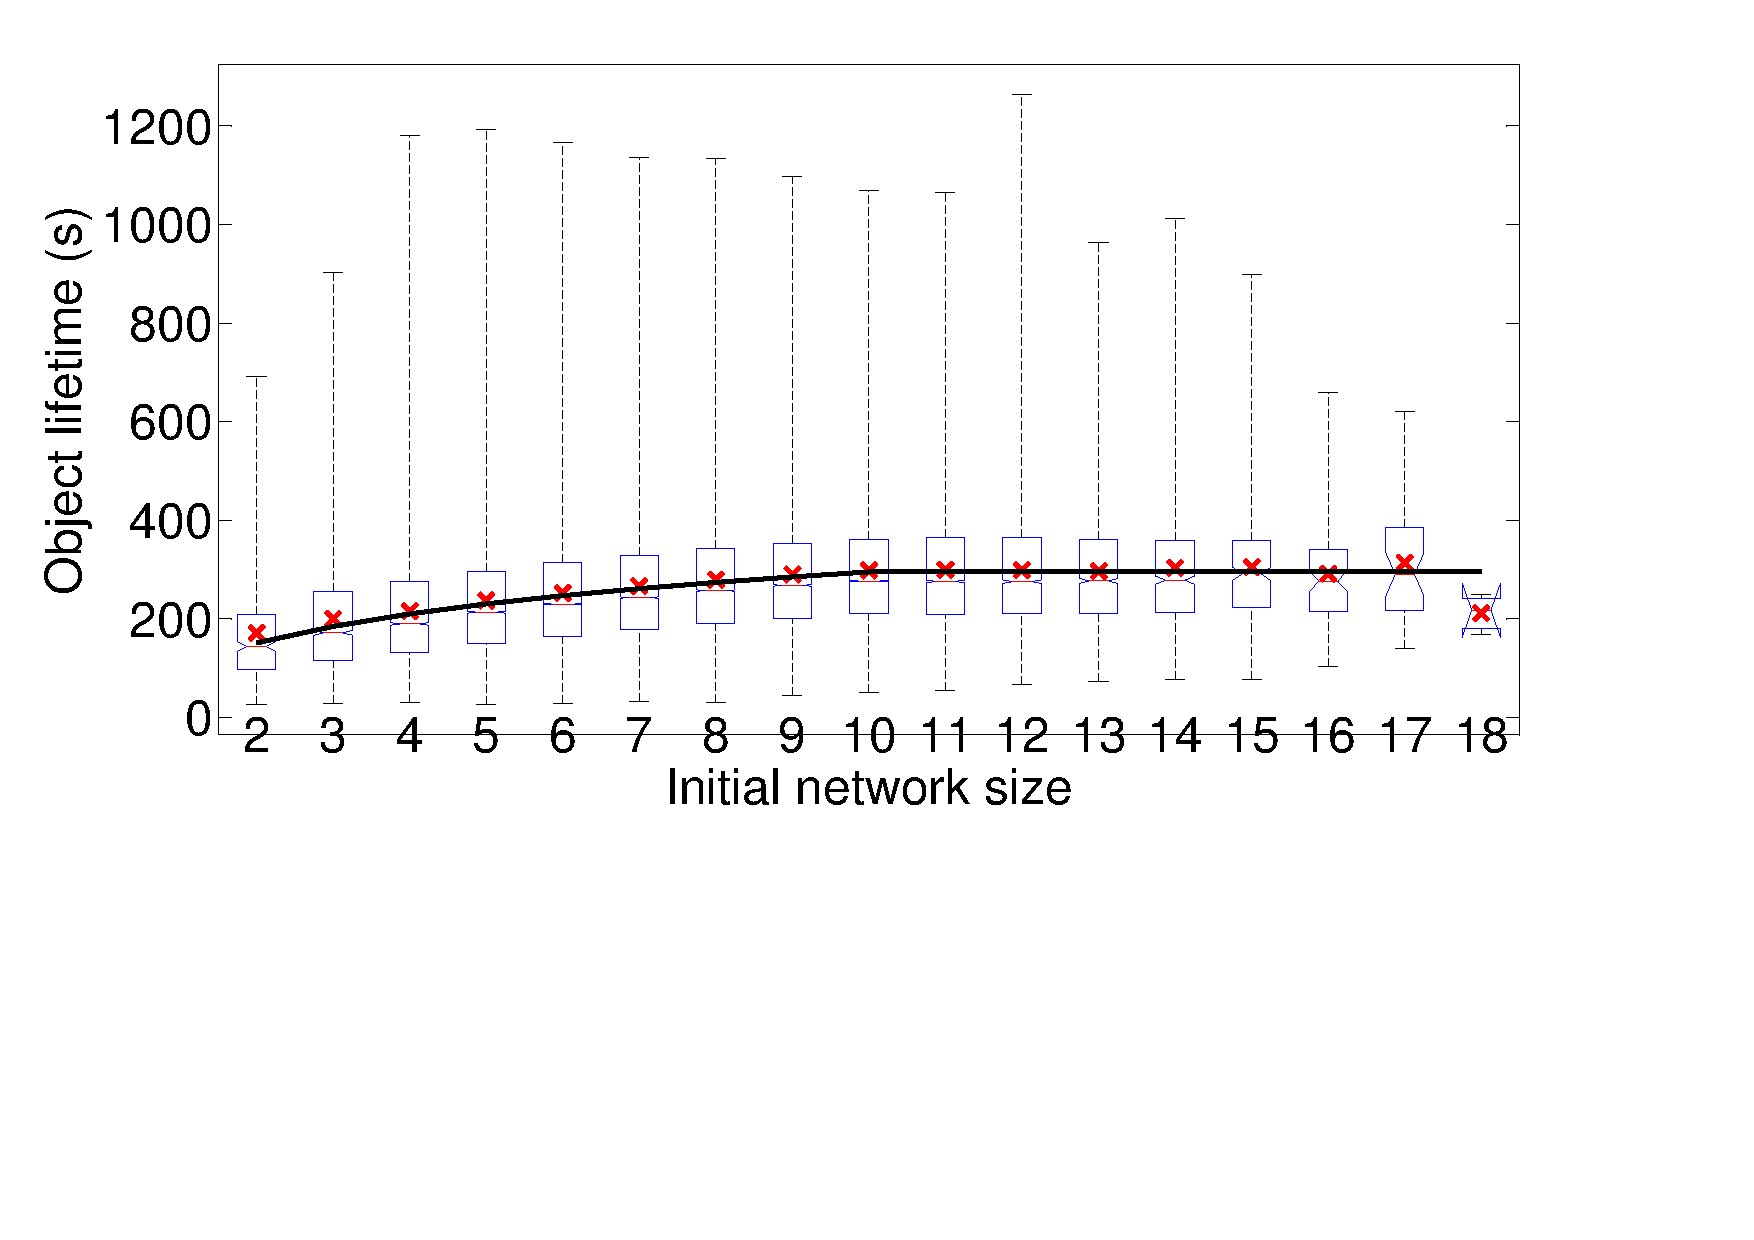
\includegraphics[clip=true, viewport=0.5cm 7.0cm 26.0cm 20.0cm, width=\columnwidth]{lifetime_simulation_model_none_100}
 \caption{Comparison of object lifetime simulation results, as a box plot, with theoretical model results for no repair, node lifetimes of $100 s$ and an average network size of 7 nodes.}
 \label{fig_lifetime_simulation_model_none_100}
\end{figure}
%
Figure \ref{fig_lifetime_simulation_model_none_100} compares the theoretical results to simulation results for the case where no repair is performed. Node have expected lifetimes of $100 s$, the number of required replicas are 10 nodes and the average network size is 7 nodes.

The expected object lifetimes as predicted by the theoretical model pass through the crosses that show the simulation data means. It can, therefore, be seen that the theoretical model matches the simulation data well for the case with no repair.

\begin{figure}[htbp]
 \centering
 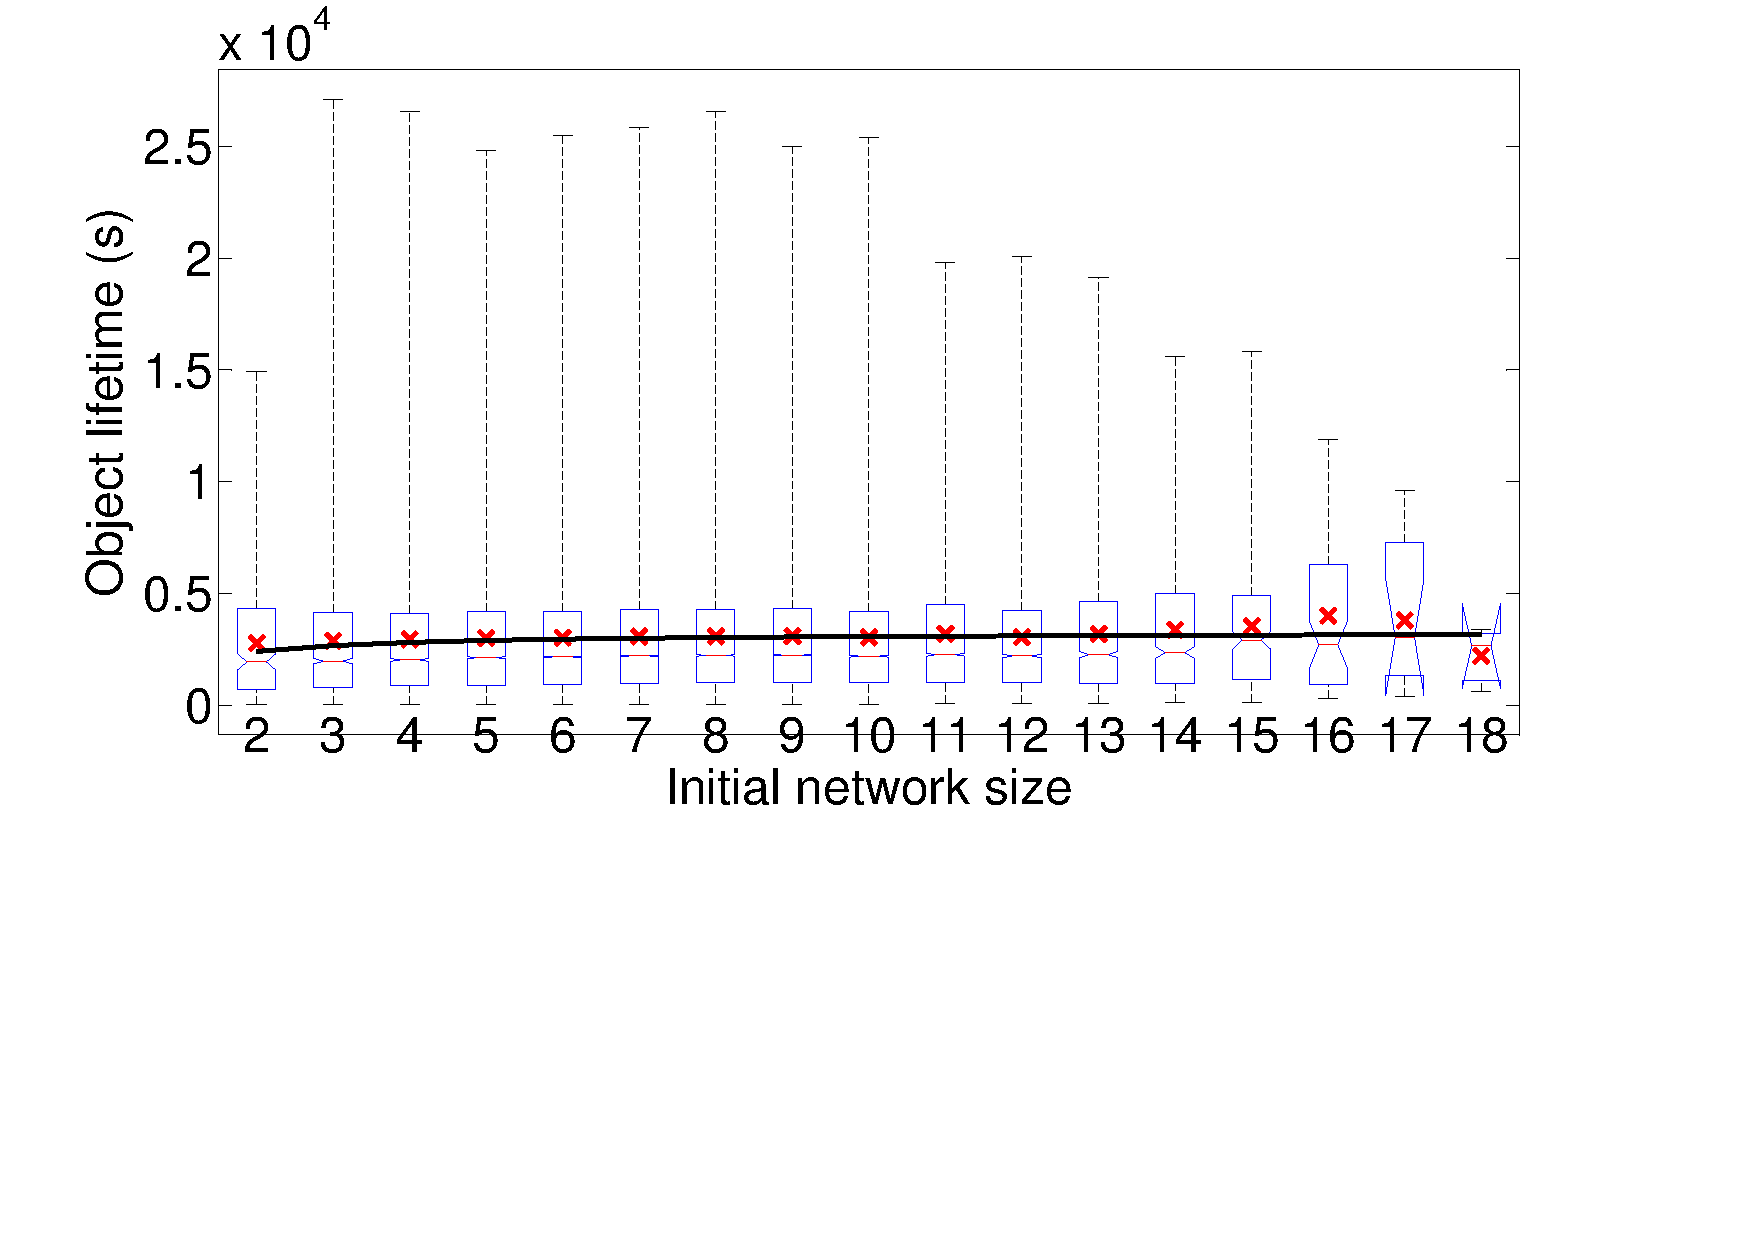
\includegraphics[clip=true, viewport=1.2cm 7.0cm 26.0cm 21cm, width=\columnwidth]{lifetime_simulation_model_20_100}
 \caption{Comparison of object lifetime simulation results, as a box plot, with theoretical model results for a repair time of $20 s$, node lifetimes of $100 s$ and an average network size of 7 nodes.}
 \label{fig_lifetime_simulation_model_20_100}
\end{figure}
%
Figure \ref{fig_lifetime_simulation_model_20_100} shows simulation data and theoretical model data for the same parameters as the previous figure, but for the case with $20 s$ repair time. A significant increase in object lifetimes can be observed. Again, the expected object lifetime as predicted by the model pass through the measured object lifetime means of the simulations. For initial network sizes on the edges of measured data, the simulation data might seem to deviate from the model data. However, in these ranges, only a few hundred measurements could be made, instead of the few thousand measurements made away from the maximum and minimum initial network size. The inaccuracy in these ranges can also be seen from the wide 5\% significance levels.

One issue that was encountered when comparing simulation data to model data was the imperfect repair scheme used in simulation. In the simulation, every $T_{\textrm{repair}}$ time, a repair of all objects in the system is initiated. In simulation, there is, however, a chance that the node that was chosen to repair an object leaves the network before the repair can complete. This reduces the effectiveness of the repair mechanism, reducing the effective repair rate. The percentage repair successes was measured during simulation and found to be $70 \%$. All repair rates in the simulation were adjusted with this number, which successfully aligned the simulation data means with the model data means.

\subsection{Conclusion}
\label{conclusion}

A Markov chain that takes network size into account when predicting object lifetimes was presented in this paper. Results show that when the average network size is comparable to the required number of replicas, object lifetimes are significantly decreased. The theoretical model was shown to be equivalent to a model that ignores network size, when the average network size is large, compared to the required number of replicas. The model was also shown to compare well to simulation, with values being nearly equal.

This paper shows how to reliably predict expected object lifetimes. When it is known that the average network size is comparable to the required number of replicas, the network size should be taken into account when modelling object lifetimes in a situation with repair. The theoretical model presented here allows for the design of a distributed storage system when the various average network sizes and node lifetime distributions are known.

Future work includes comparing object lifetimes using replication, with object lifetimes using erasure coding as redundancy technique. Modelling object lifetimes using heavy-tailed node lifetime distributions, such as the Pareto distribution, is also required. The variable failure rate of the Pareto distribution complicates modelling it as a Markov chain.
    
\section{Overhead}
\section{Fairness}

\begin{figure}[htbp]
 \centering
 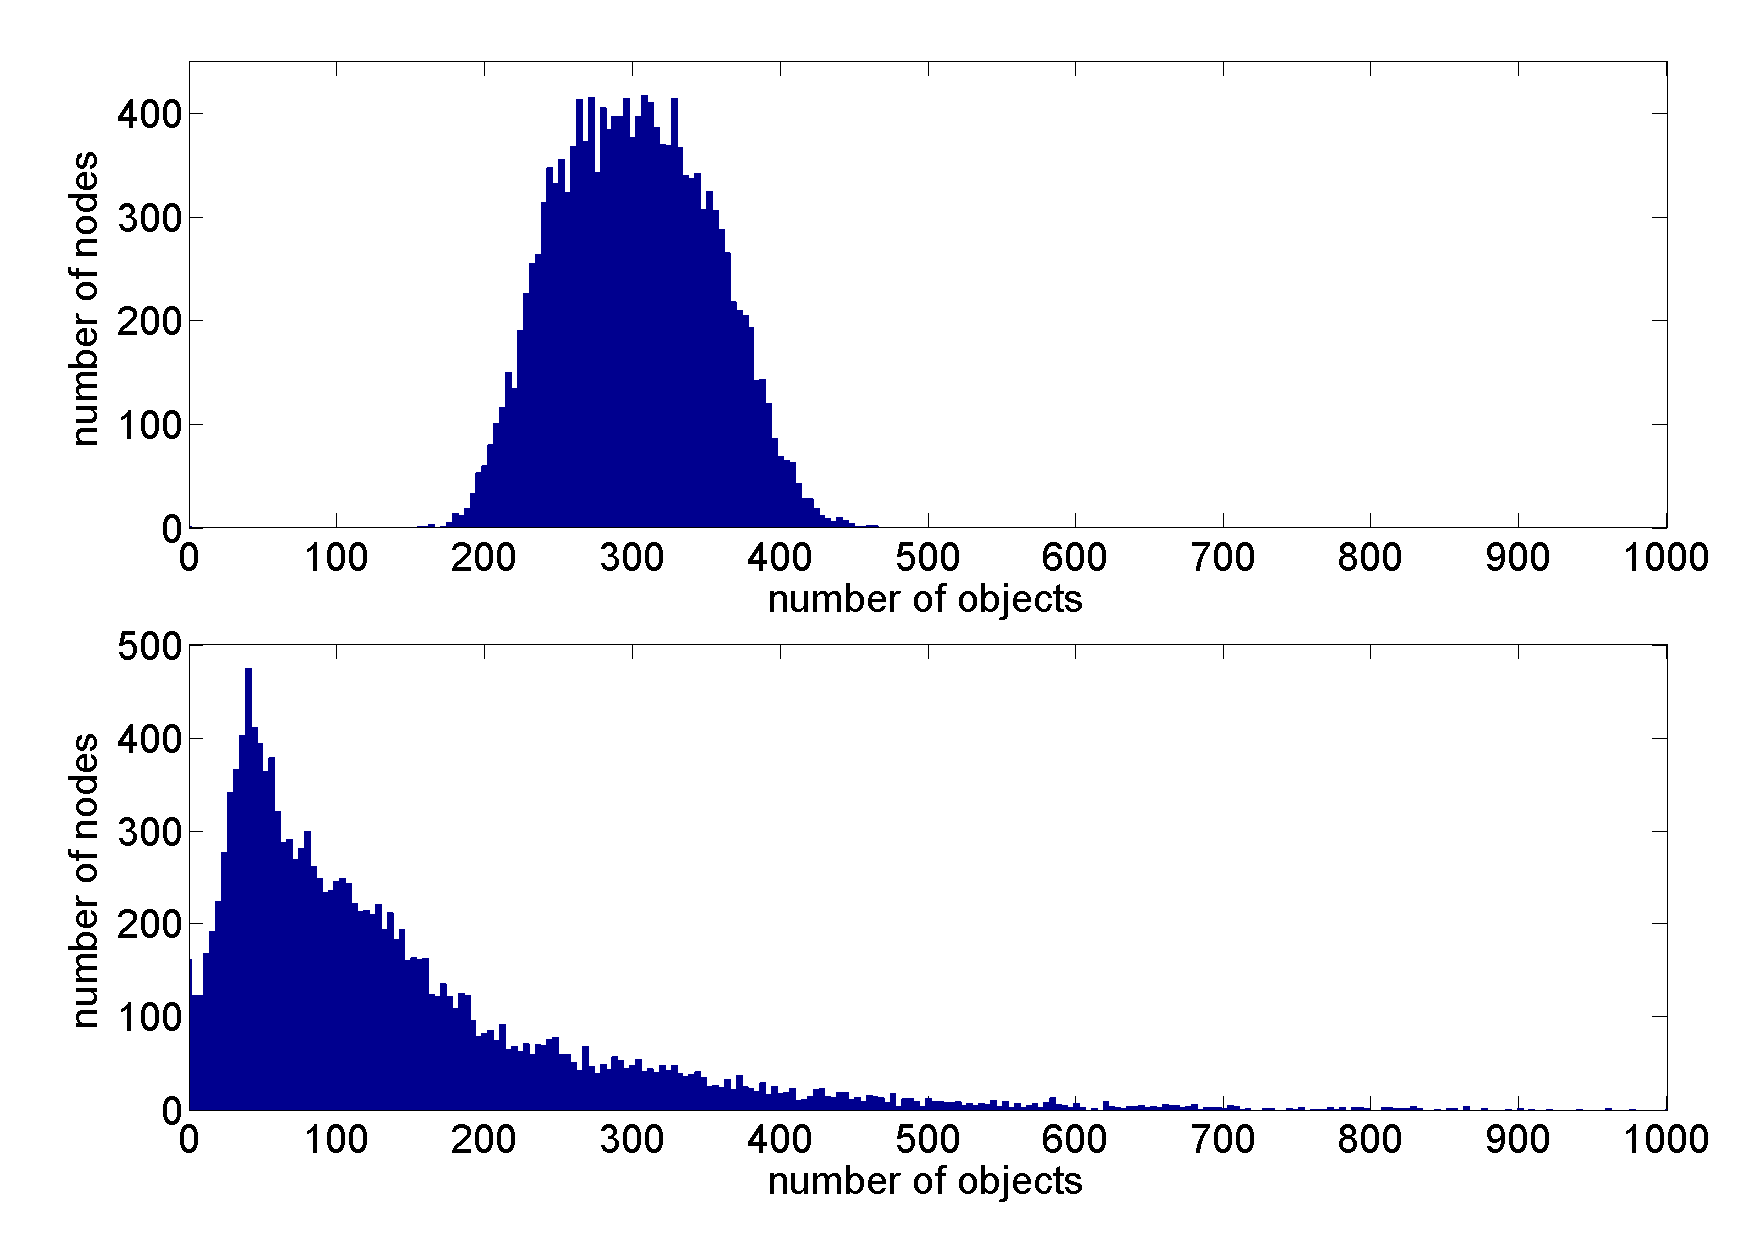
\includegraphics[clip=true, viewport=1cm 0.5cm 28.5cm 20cm, width=\columnwidth]{RootRepOverlayObjects}
 \caption{(top) Root/Replica object number distribution, (bottom) overlay number distribution.}
 \label{fig_group_overlay_objects}
\end{figure}
%
To evaluate the fairness, we evaluate the standard deviation of the number of objects stored per peer. Figure \ref{fig_group_overlay_objects} (top)
shows the distribution of group objects over nodes in the network. The figure shows how many nodes store how many objects. The distribution has a
mean and standard deviation of 302 and 51 objects per node respectively.

Figure \ref{fig_group_overlay_objects} (bottom) shows the distribution of overlay objects in Pithos with a mean and standard deviation of 153 and 189
objects per node respectively. Comparing the standard deviations of group storage to overlay storage, it appears that group storage is much fairer
than overlay storage. This shows that by designing a hybrid system which prefers group storage to overlay storage, one is also designing a fairer
system than overlay storage.

\begin{figure}[htbp]
 \centering
 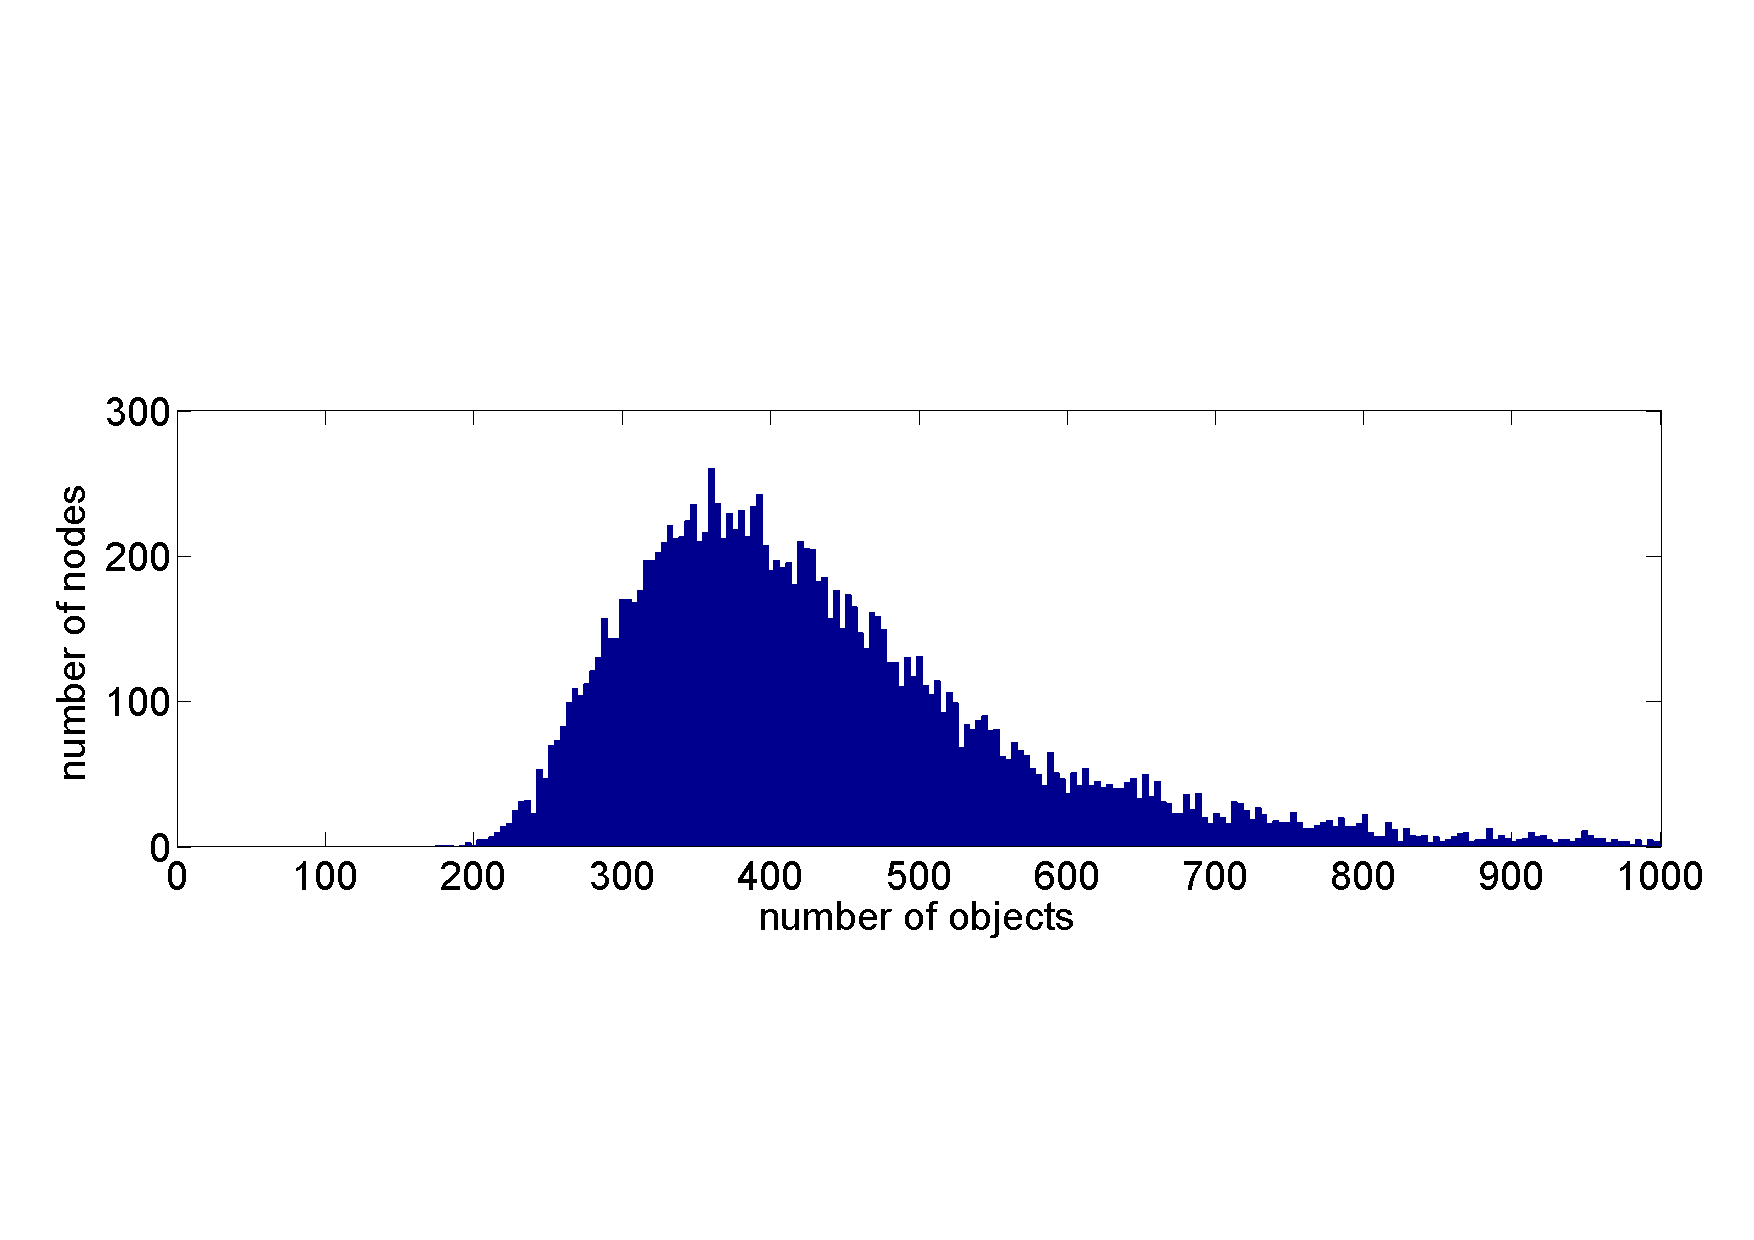
\includegraphics[clip=true, viewport=1cm 5cm 29cm 14.5cm, width=\columnwidth]{Objects}
 \caption{Combined object number distribution}
 \label{fig_objects}
\end{figure}
%
Figure \ref{fig_objects} shows the combined object distribution of Pithos, with a mean and standard deviation of 453 and 200 objects per node
respectively. This shows that the fairness of Pithos is currently dominated by the fairness of Pastry and that Pithos is as fair as overlay storage.

\section{Responsiveness}
    To exactly compare Pithos with overlay storage, the probability that a message is routed within a group ($P(g)$) should first be known. It is
expected that $P(g)$ will be different for MMVEs with different defining mechanics. It should be possible to determine $P(g)$ experimentally for a
specific type of game, but this will require access to the game client of an already implemented P2P MMVE. The exact measurement of $P(g)$ is left
for future work, but the responsiveness can be calculated as a function of $P(g)$. Working with a function in $P(g)$ also allows for the
implementation of various dynamic strategies that can adapt to various values of $P(g)$.

We define $P(o) = 1 - P(g)$ as the probability that a message is routed within the overlay. We define $T_{\textrm{group}}$ as the root and replica
message distribution and $T_{\textrm{overlay}}$ as the overlay message distribution, both shown in Figure \ref{fig_pithos_response}. The expected
value of the overall system response time ($E[T_{\textrm{resp}}]$) can then be presented as a weighted average of the expected values of both the
group and overlay storage distributions, as follows:
%
\begin{align}
    E[T_{\textrm{resp}}] &= P(g)\left(E\left[T_{\textrm{group}}\right]\right) + P(o)\left(E\left[T_{\textrm{overlay}}\right]\right)\notag\\
                         &= P(g)\left(E\left[T_{\textrm{group}}\right]\right) + \left[1 - P(g)\right]\left(E\left[T_{\textrm{overlay}}\right]\right).\label{expected_response_time}
\end{align}

\begin{figure}[htbp]
 \centering
 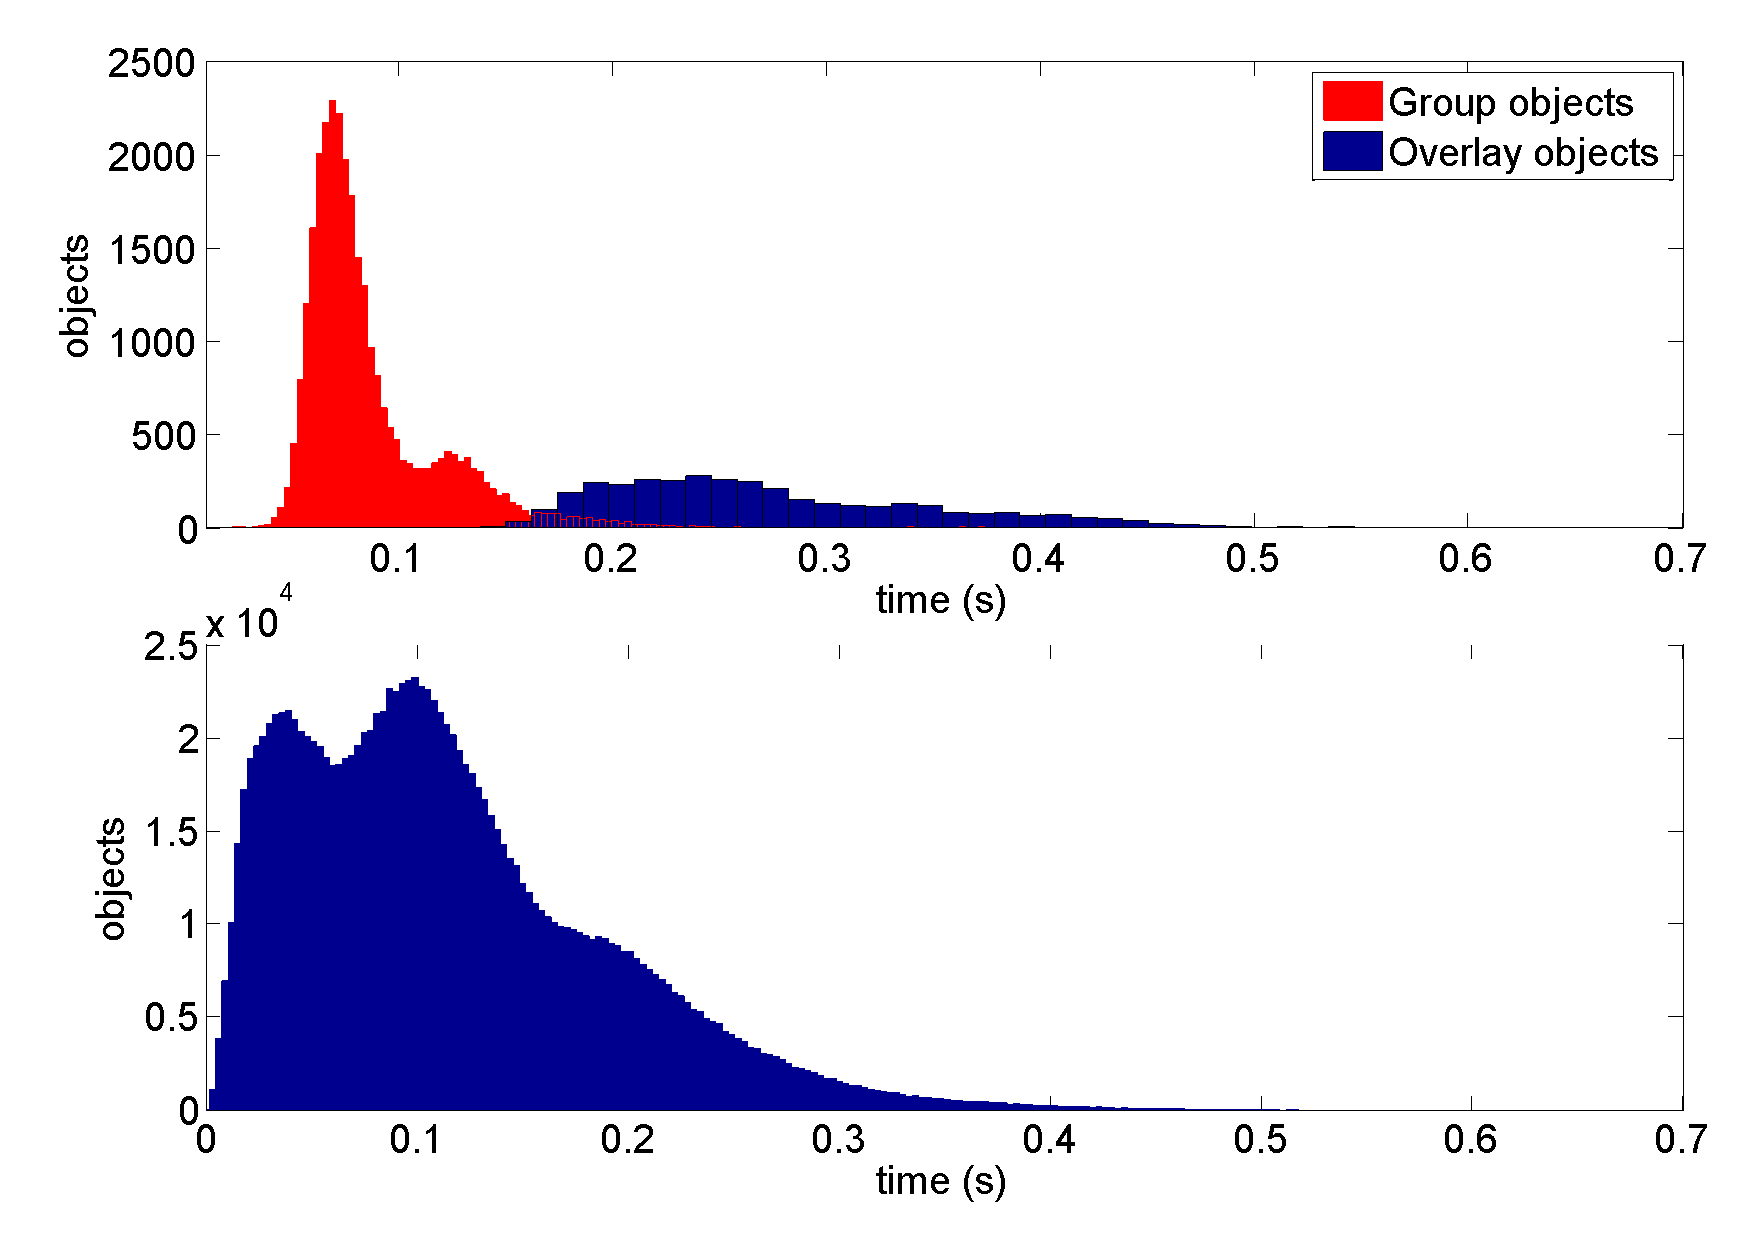
\includegraphics[clip=true, viewport=1cm 0.5cm 29cm 20.5cm, width=\columnwidth]{StoreTimes}
 \caption{(top) Time distribution of overlay and root/replica objects, (bottom) time distribution of Pastry objects.}
 \label{fig_pithos_response}
\end{figure}
%
Figure \ref{fig_pithos_response} (top) shows the distribution of mean storage request times over all nodes in the Pithos network for the different
storage types. One can see that the intra-group root and replica objects are stored much faster ($E\left[T_{\textrm{group}}\right] = 0.0878s$) than
the overlay objects in the network ($E\left[T_{\textrm{overlay}}\right] = 0.328s$). Figure \ref{fig_pithos_response} (bottom) presents the
responsiveness of a pure Pastry network of 14999 nodes in Oversim. The simulated Pastry network was found to have a mean routing time of $0.12s$.

The responsiveness of Pithos will depend on the responsiveness of Pastry, where the expected number of Pastry hops are given by:
\cite{storage_and_chaching_PAST}:
%
\begin{equation}\label{pastry_hops}
    E[H_{\textrm{pastry}}] = \log_{2^b}\left(N\right),
\end{equation}
%
where $b$ is a network parameter that is usually chosen as $b = 4$. From this, it is possible to calculate a theoretical performance for Pithos and
compare that with a theoretical performance of overlay storage.

When using a weighted hop average, as with Equation \eqref{expected_response_time}, the expected number of Pithos hops is given by:
%
\begin{equation}\label{expected_response_time}
    E[H_{\textrm{pithos}}] = P(g)\left(E\left[H_{\textrm{group}}\right]\right) + P(o)\left(E\left[H_{\textrm{overlay}}\right]\right),
\end{equation}
%
where $E\left[H_{\textrm{group}}\right]$ is the expected number of group hops and $E\left[H_{\textrm{overlay}}\right]$ is the expected number of
overly hops. In Pithos, $E\left[H_{\textrm{group}}\right] = 1$, because in a fully connected group any node is always one hop away from any other
node.

To find the value of $E\left[H_{\textrm{overlay}}\right]$, one has to consider how many hops an overlay message requires in Pithos. One hop is
required to send a store request from a group peer to its super peer. The super peer then forwards the message to another super peer in
$\log_{16}(M)$ hops, from Equation \eqref{pastry_hops}, where $M$ is the number of super peers in the network. From the destination super peer,
another hop is required to send the message to the destination group peer. This gives:
%
\begin{equation}\label{group_hops}
    E\left[H_{\textrm{overlay}}\right] = 1 + \log_{2^b}(M) + 1.
\end{equation}
%
Equation \eqref{expected_response_time} then becomes:
%
\begin{align}
E[H_{\textrm{pithos}}] &= P(g) + \left[1 - P(g)\right]\left[2 + \log_{16}\left(M\right)\right]\notag\\
                       &= 1 + \left[1 - P(g)\right] + \left[1 - P(g)\right]\left[\log_{16}(M)\right]\notag\\
                       &= 1 + \left[1 - P(g)\right]\left[1 + \log_{16}(M)\right]\notag\\
                       &= 1 + P(o)\left[1 + \log_{16}(M)\right].\label{expected_response_time_exp}
\end{align}

\begin{figure}[htbp]
 \centering
 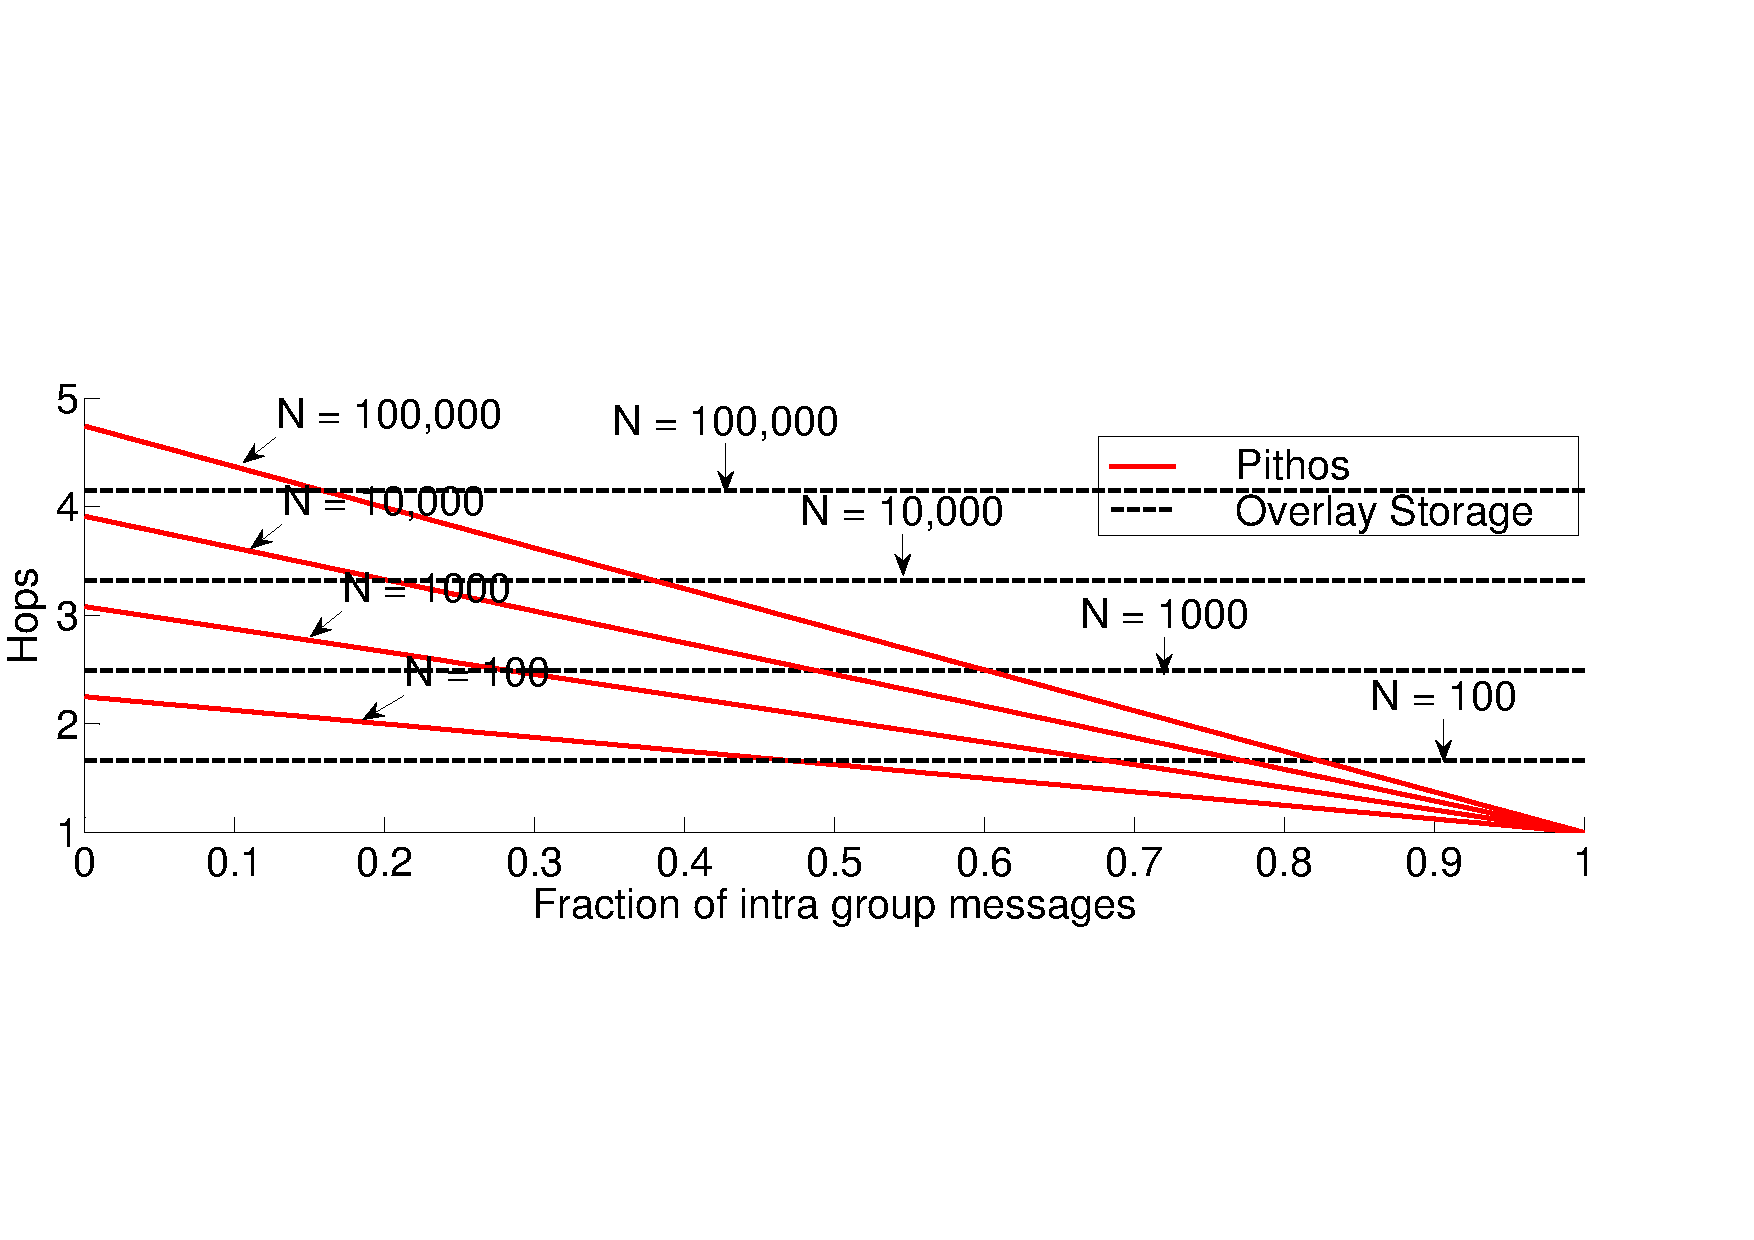
\includegraphics[clip=true, viewport=0cm 5cm 27cm 14.5cm, width=\columnwidth]{Hops_vsGroupFrac_4n}
 \caption{Expected number of Pithos hops, compared to the expected number of overlay hops, as a function of $P(g)$ for various values of $N$}
 \label{fig_hop_compare}
\end{figure}
%
Figure \ref{fig_hop_compare} compares the expected number of Pithos hops with the expected number of overlay hops as a function of intra-group
probability ($P(g)$) for various numbers of nodes ($N$). The overlay hops were calculated from Equation \eqref{pastry_hops}, while the Pithos hops
were calculated from Equation \eqref{expected_response_time_exp}. For the Pithos graphs, an average number of 50 peers per group was used to
determine the number of super peers.

Figure \ref{fig_hop_compare} shows that for a low value of $P(g)$, overlay storage performs better than Pithos because of the additional two hops
present in Pithos. High values for $P(g)$ are expected, because of the distance-based design of Pithos that attempts to maximise the value of $P(g)$.
This should have Pithos perform better than overlay storage.
\chapter{Pithos evaluation}
    \label{chp:EVALUATION}

    %%%%%%%%%%%%%%%%%%%%%%%%%%%%%%%%%%%%%%%%%%%%%%%%%%%%%%%%%%%%%%%%%%%%%%%
    \section{Performance}

    \subsection{Bandwidth requirements (overhead)}
    %Mention something about low bandwidth links and how that influences timeout and what extra mechanisms were required.
    %Check how this increases with increased network sizes and varying levels of network churn.

        \subsection{Group consistency}
        %Check how this increases with increased network sizes and varying levels of network churn.

    \section{Metrics}

    \section{Theoretical results}

    \section{PithosTestApp}

    \section{Comparison between theoretical and simulation results}

        \subsection{Overhead}
        \subsection{Fairness}
        \subsection{Reliability}
        \subsection{Responsiveness}

    \section{Comparison between Pithos and other architectures}

        \subsection{Overhead}
        \subsection{Fairness}
        \subsection{Reliability}
        \subsection{Responsiveness}

\chapter{Conclusions and Recommendations}
\label{chp:CONC}

This work focussed on developing a state management architecture for P2P MMVEs. In order to do this, an understanding was required of P2P networks, MMVEs and what the main challenges of P2P MMVEs are.  It was found that state management and persistency is used by the consistency architecture and, therefore, that the consistency architecture implicitly specifies the storage requirements.

After having identified the requirements of a state management and persistency architecture, related work was reviewed and compared against the identified requirements. This allowed us to identify areas where improvements might be made.

The design of Pithos was presented in order to satisfy all identified requirements, presenting every aspect of Pithos in terms of the requirement identified. The Pithos use case was reviewed and presented as a distributed storage system and the mechanisms to implement the use cases were discussed.

With the conceptual design finalised, the implementation specifics were reviewed. Pithos has been implemented as an Oversim simulation that allows for large scale simulations. Some implementation issues that were reviewed were maintaining group consistency as well as persistency in group storage. An evaluation was performed in order to verify that Pithos satisfies all the requirements originally identified.

When Pithos was evaluated for various churn levels and repair rates, it was seen that many factors influence reliability. The factors influencing reliability were found to be directly related to expected object lifetime. A Markov chain model was developed to allow for the prediction of expected object lifetimes. It was found that the literature reviewed assumed an infinite network size and does not take limited network sizes into account. Comparing our model with simulation results, it was found that finite group sizes does affect object lifetimes when the average group size is small, compared to the required number of replicas.

\section{State consistency}

The generic consistency model developed provides a framework for the design and development of MMVEs in general. Because many aspects of the generic consistency model are trivial in C/S models, the model is perhaps more applicable to a P2P MMVE

\section{State management}

\section{Pithos}


\section{Further work}
\label{further_work}


%==== Appendices ====================================================
%\appendix
%\appendixpage\relax

%\chapter{Ensuring group consistency in Pithos}
\label{chp:GROUP_INCONSISTENCY}

This appendix described, in chronological order, the steps taken to ensure group consistency. It provides initial findings, discusses the reasons for inconsistency and introduces the proposed solutions.

\section{Initial approach}
The initial approach to achieve group consistency was to have every peer inform all other peers when it was moving from one group to another. If a peer is removed from the network due to churn, another peer has to discover that the peer has left, which is done with timeouts. If a request times out, the peer making the request informs the group of the peer that left.

\begin{figure}[htbp]
 \centering
 \includegraphics[clip=true, viewport=0mm 0mm 460mm 212mm, width=\columnwidth]{gc_first}
 \caption{Group consistency before any improvements}
 \label{fig_gc_first}
\end{figure}
%
Figure \ref{fig_gc_first} shows an enlarged view of the perceived group size of every node in the group for the initial group consistency scheme. The lines running across the graph is due to nodes leaving the network and joining again at a later time.

From approximately 2925 s, a new peer joins the group and reports the group size as eight, when all other peers report the group size as seven. Multiple variations of these inconsistencies occurred during testing. A primary source of inconsistencies was the fact that it takes time to inform all group peers of a peer that left and that it takes time to inform all group peers of a peer that joined.

Issues also occurred because of how newly stored objects are handled. When a new peer joins the group, it starts to generate objects. The group super peer sends a joining peer a list of group peers. After this occurs, the group peers are informed of the new peer. A peer joining a group can immediately start to store objects at the request of other peers. This can happen before some peers are aware of the joining peer. The unaware peers will then get a message saying that an object has been stored on the new peer, before they are aware of the new peer. The solution was to assume that an object was generated by a valid peer and to add any unknown peer information contained in an object add message to the peers list in the group ledger.

Group inconsistency can arise because there might be some latent object add messages still enroute to peers, after the peer has already left the network and informed other peers of its leaving. This means that a peer has already left, but after it informed the group peers of its leaving and all group peers have removed the peer from memory, the group peers receive a message for an object that is supposedly now stored on the peer that just left. The mechanism mentioned above is initiated and the, now unknown, peer is again added to the peer list.

Many transient group states that led to inconsistencies were solved by the super peer storing the information of the last peer that left and the last peer that joined. Every time a new peer joins, the super peer informs the joining peer of the last peer that left. This allows the joining peer to ignore any latent object add messages received from the leaving peer. Any messages received from the last peer that left are ignored. This prevents latent messages from peers that left to affect the group view of peers.

\section{Peer starvation problem}
\begin{figure}[htbp]
 \centering
 \includegraphics[clip=true, viewport=0mm 0mm 455mm 212mm, width=\columnwidth]{gc_middle}
 \caption{Group consistency with starvation}
 \label{fig_gc_middle}
\end{figure}
%
The mentioned improvements created the issue shown in Figure \ref{fig_gc_middle}, where a peer will believe that another peer has left. The group will be informed of the peer that supposedly left, but is actually still present in the group. Because all peers will now ignore messages from the peer that supposedly left, including the super peer, all requests sent by the peer that supposedly left will be ignored. The requests will then timeout on the ignored peer and the ignored peer will remove all group peers. This isolates the peer and prevents any requests from being serviced.

The starvation was caused by peers not responding to requests. A scenario could occur where a peer did not contain a requested object or where the network bandwidth was limited, which prevented a response from arriving at a peer before the request timeout expired. In either of these two situation, the peer making the request was under the impression that the target peer had left the network. It then informed all other peers of this.

The solution to this issue was to adjust the timeout as a function of the available network bandwidth and to make sure every node always responded to a request, whether as a success or failure. Functionality was also added to the super peer to check whether a peer that was reported as having left, actually did leave the network.

Other issues were caused when group migration was enabled. A node might leave a group to move to another, but as the node leaves some peer that has not been informed of the peer leaving would make a request form the leaving peer. The leaving peer would respond to that request, which would have the requesting peer add the peer back into the group. This could cause the situation where peers existed in multiple groups.

The solution to this was to include the group membership information in every request message. A peer's membership can be uniquely identified by the IP address and port of the group's super peer. If a peer receives a message with a different group address than its own, it ensures that that peer is not part of its group.

This also solved the case where Peer A requested an object from Peer B, just as Peer B was leaving the group. Peer B will already be in its new group when receiving the request from Peer A. Peer B will see that the request originated from outside its group, so will not add the new peer to its group. If it contains the requested object, it will however still respond with the object. When Peer A receives the object, it will detect that it was sent from another group and remove Peer B from its group ledger. In this way, the request was successfully handled and group consistency is maintained.

\section{Final solution}
\begin{figure}[htbp]
 \centering
 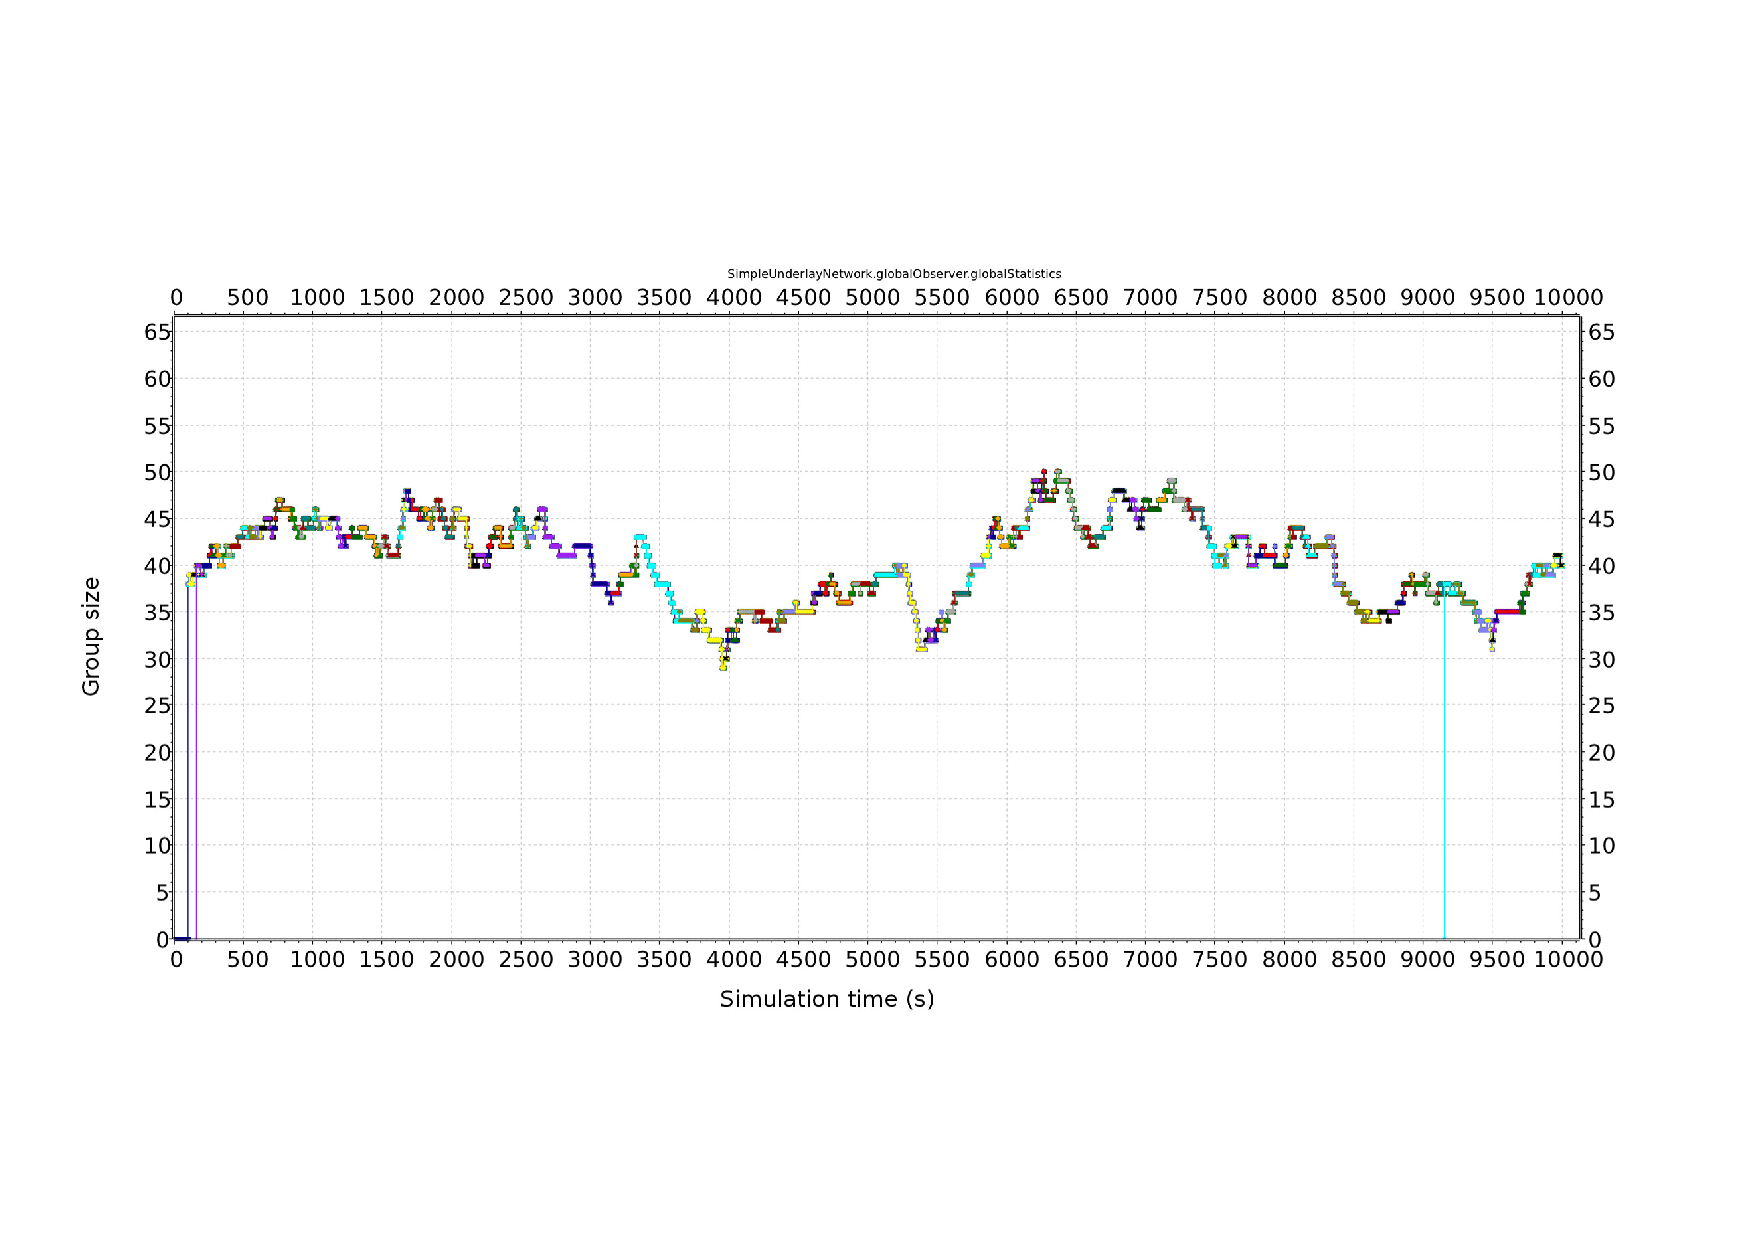
\includegraphics[clip=true, viewport=12mm 35mm 275mm 165mm, width=\columnwidth]{gc_final_png}
 \caption{Group consistency after all improvements}
 \label{fig_gc_final_app}
\end{figure}
%
Figure \ref{fig_gc_final_app} shows the group consistency after all improvements were added for a larger group than the previous two. Even with the larger group, complete consistency is achieved.

When object lifetime was tested, all requests were stopped after a certain period of time to speed up the simulation. This created an issue where group peers did not become aware of peers leaving the group, because no peers sent requests that could timeout. This prompted the addition of keep-alive messages.

Regular keep alive messages are sent to peers. If a peer does not respond to the message, that peer is removed from the group. The time between keep alive messages can be adjusted as a function of network churn. In order to reduce the load on the super peer, each peer randomly chooses a target peer and sends a keep-alive message, as explained in Section \ref{leave_design}.


%==== Bibliography acro's & Index ===================================
%\backmatter

%\newpage
%\IEEEtriggeratref{43} %Balance the bibliography
\bibliographystyle{IEEEtran}
\bibliography{../BibTeX/P2P_MMOG}

\end{document}
